% !TeX spellcheck = en_US
\documentclass[a4paper, 12pt]{article}
\usepackage[utf8]{inputenc}
\usepackage{newtxtext}
%\usepackage{easyReview}
\usepackage[english]{babel}
\usepackage{graphicx}
\usepackage{xcolor}
%\usepackage{noto}
%\usepackage{notomath}
%\usepackage{libertinus}
\usepackage[a4paper,left=3cm,right=3cm,top=3cm,bottom=3cm,bindingoffset=5mm]{geometry} %page setting
\usepackage[colorlinks, linkcolor = purple, citecolor = black, filecolor = blue, urlcolor = blue]{hyperref} %hyperref settings
%\usepackage[colorlinks = false]{hyperref}
%\usepackage[hidelinks]{hyperref}
\usepackage{rotating}
\usepackage{caption}
\usepackage{subcaption}
\usepackage[capposition=top]{floatrow}
\usepackage[sectionbib]{natbib}
\usepackage[globalcitecopy]{bibunits}
\defaultbibliography{biblio.bib}
\usepackage{setspace}
\usepackage{csquotes}
\usepackage{todonotes}
%\usepackage{amsmath}
\usepackage{amssymb}
\usepackage{booktabs}
\usepackage{svg}
\usepackage{amsmath}
	\DeclareMathOperator*{\E}{\mathbb{E}}
\usepackage{bm} %bold math symbols
\usepackage{tikz}
	\usetikzlibrary{bayesnet}
\usepackage{chngcntr}

%\usepackage{lmodern} % Use Latin Modern fonts

\newenvironment{customabstract}
{\begin{center}\begin{minipage}{0.85\textwidth}}
		{\end{minipage}\end{center}}
%\usepackage[capposition=top]{floatrow}
\usepackage[most]{tcolorbox}
\usepackage{float}
\restylefloat{table}

%\onehalfspace
\begin{document}
	

%\title{Going viral: How media coverage of inflation narratives affects the macroeconomy\\ \textit{\textcolor{purple}{Prelimininary and incomplete draft.\\ Please do not cite!}}}
\title{Going Viral: Inflation Narratives and the Macroeconomy}
\author{Max Weinig\footnote{\textbf{Corresponding author}. Universität Hamburg, email:  \href{mailto:max.weinig@uni-hamburg.de}{max.weinig@uni-hamburg.de}} \and Ulrich Fritsche\footnote{Universität Hamburg \&KOF ETH Zurich, email: \href{mailto:ulrich.fritsche@uni-hamburg.de}{ulrich.fritsche@uni-hamburg.de}}}
\date{\today}

\maketitle

\begin{abstract}
    \noindent In recent years, there has been increasing interest in the analysis of narratives in macroeconomic research. Our paper contributes to this research by proposing a way to identify and extract economic narratives from media reports. Therefore, this paper applies state-of-the-art text analysis methods to a large news corpus covering five years of news coverage in combination with results from a survey study on recent inflation narratives \citep{Andre.2023} in the US. This approach enables us to measure the prevalence and spread of inflation narratives over time and to examine the role of these narratives in aggregate macroeconomic expectations. Using Granger causality tests and local projections, we provide empirical evidence on the dynamics between inflation narratives and inflation expectations. Moreover, the paper highlights the vast heterogeneity across short-term and mid-term inflation expectations as well as socioeconomic groups. \\
    \\
    \textbf{JEL codes:} D84, E31, E32, E52, E71\\
    \textbf{Keywords:} narratives, expectations, inflation, media, textual data, machine learning
\end{abstract}
\vspace{4cm}
\begin{customabstract}
 \footnotesize
	 \noindent We thank Sami Diaf, Victoria Hünewaldt, and Lisa Wegner for their very helpful comments. Furthermore, we thank seminar audiences at the International Conference on Computational Statistics, the International Conference on Macroeconomic Analysis and International Finance, the Narrative Economics Alliance Ruhr, the University of Gießen, the KOF Swiss Economic Institute of the ETH Zürich, the Forum for Macroeconomics and Macroeconomic Policies, and the IMK Macroeconomic Policy Institute Workshop for their comments. 
	
\end{customabstract}




% Hier Introduction (new page)
\newpage

% !TeX spellcheck = en_US
\section{Introduction}\label{sec:Intro}

For the first time in decades, numerous countries world-wide, including the United States, are facing high inflation rates. This is important because households generally perceive high inflation as one of the most important (economic) policy issues \citep{Shiller.1997, Stantcheva.2024}. While some inflation might be desirable, rates way above the two percent target impose substantial costs on society \citep{Romer.2012}. Consequently, its origin and the underlying mechanisms have been and continue to be subject of ongoing debate. \cite{Blanchard.2023} attribute the increase in inflation to a combination of supply constraints and robust aggregate demand. \cite{Reis.2022} highlights an ``overly long period of expansionary policy'', and central banks tolerating higher inflation rates. \cite{Weber.2023} discuss the role of market power to hike prices, which indicates ``sellers' inflation''. On a theoretical level, \cite{Werning.2023} provide a decomposition of inflation and argue that the general cause of inflation is conflict or disagreement. Expectations are of great importance in their conceptualization, as they shape the aspirations of workers and firms.

%\begin{figure}[H]
%	\centering
%	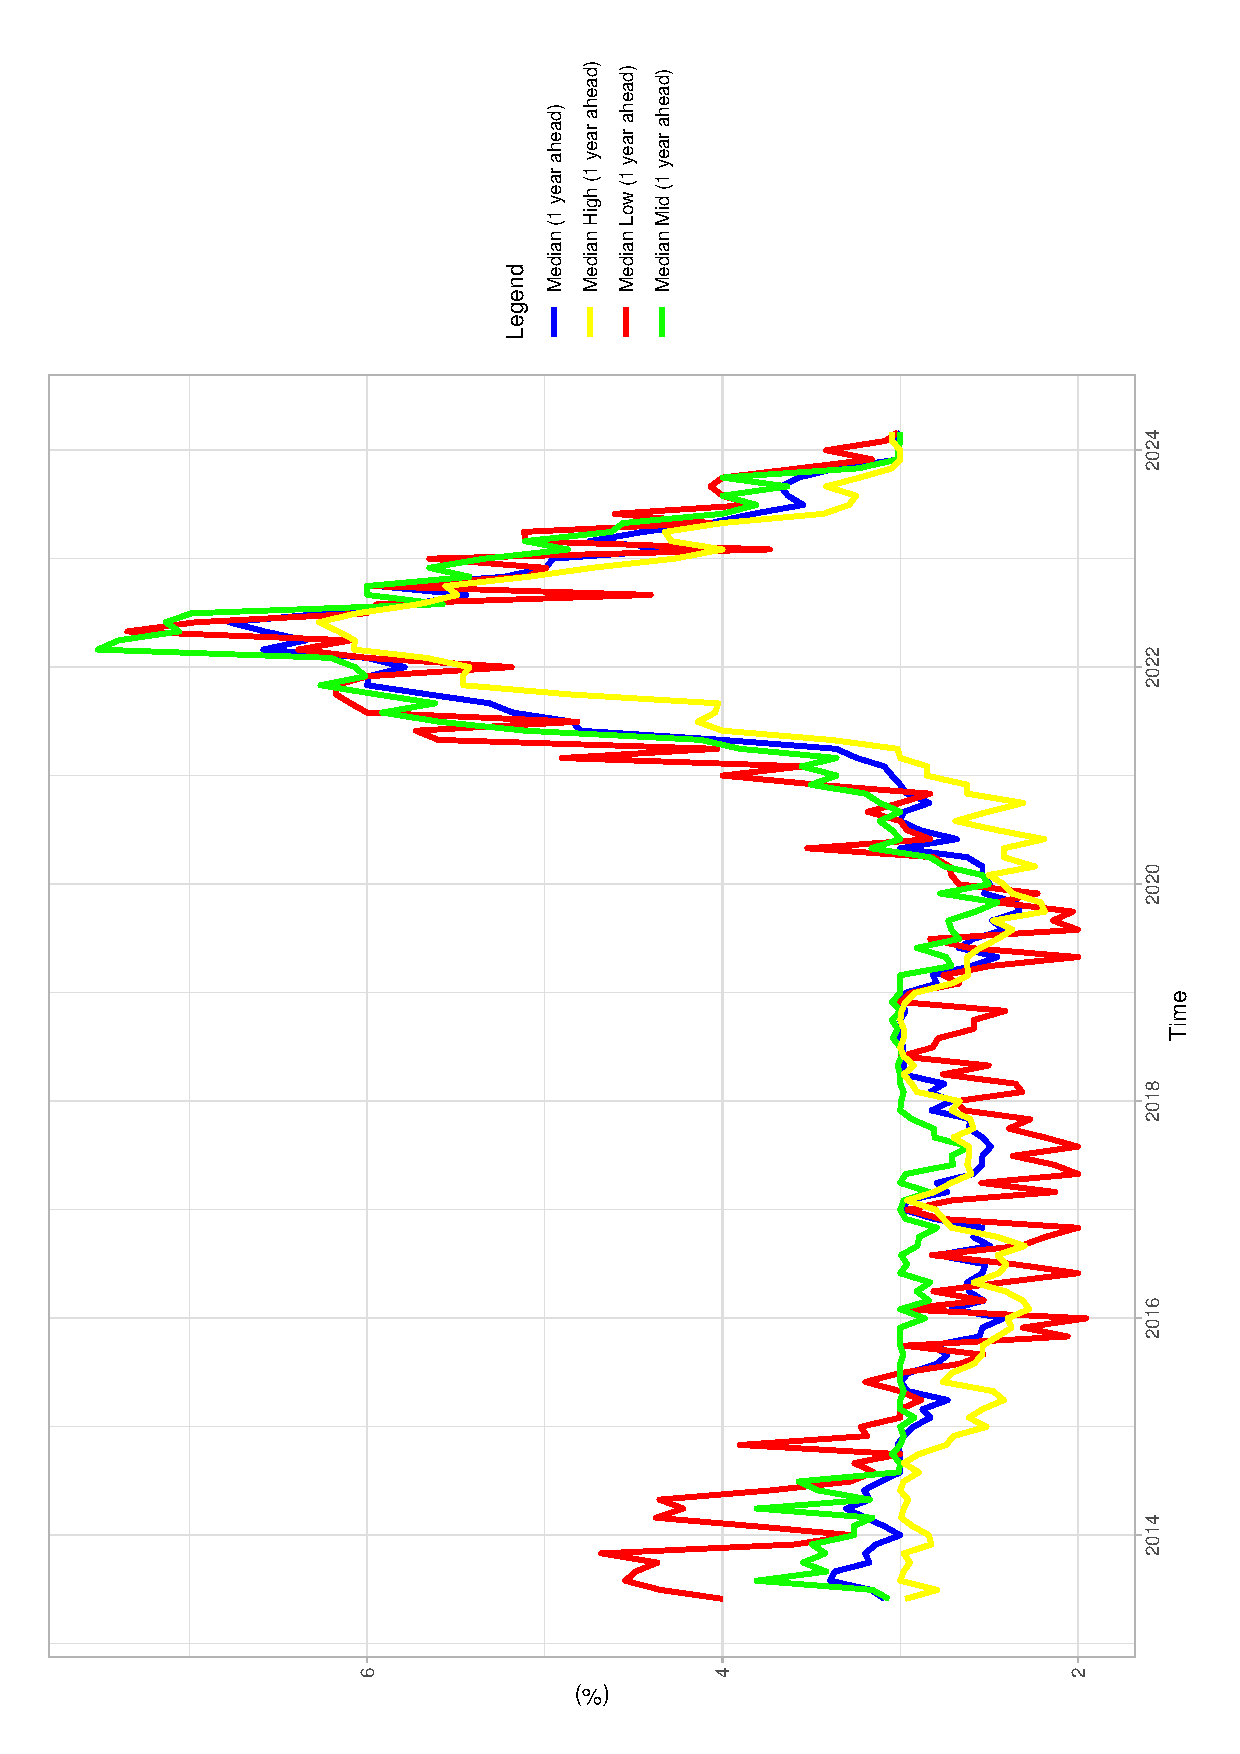
\includegraphics[width=0.95\linewidth]{figures/infl_expect.png}
%	\caption{Median inflation expectations of US households}
%	\label{fig:inflexpect}
%	\floatfoot{Note: Median survey-based inflation expectations of US households one and three years ahead. Source: New York Fed Survey, see \cite{Armantier.etal.2017} for details.} 
%\end{figure}

In standard New Keynesian models, this idea of forward-looking agents is essential, as \cite{Werning.2022} demonstrates. In these models, expectations are seen as a driver of inflation dynamics. Influential on forward-guidance was the work by \cite{Krugman.1998}, who proposed that during a liquidity trap, central banks should be able to stimulate the economy by raising inflation expectations through credibility. This is why central banks closely monitor the expectations of households, firms, and experts— or, as Jerome Powell, the current Chair of the Federal Reserve, puts it: ``Our monetary policy framework emphasizes the importance of well-anchored inflation expectations, both to foster price stability and to enhance our ability to promote our broad-based and inclusive maximum employment objective.'' \citep{Powell.2021}. 

A long tradition of empirical economic research addresses the question of whether and to what extent the expectations of households influence economic decisions. Two moments are subjects of interest: the consumption-saving nexus in the Euler-Equation and inflation uncertainty as a precautionary saving motive \citep{DAcunto.2023}. Regarding the former, work by \cite{Juster.1972} suggested already in the 1970s that inflation expectations influence expenditure spent on durable goods, while the findings fo \cite{Burch.1975} indicate a strong relationship between inflation expectations and the national saving rate. More recent research by \cite{Bachmann.2015} is also in line with both moments. The authors do report a significant negative relationship between expectations and savings, but only for a subset of households, whose expectations are within one percentage point of the actual realized inflation. By linking survey data on inflation expectations of households to administrative data, \cite{Vellekoop.2019} report a negative relationship between inflation expectations and net worth. With a pseudo-panel study, the results of \cite{Duca.2021} are in line with the Euler equation for all participants, however, smaller effect sizes for more inaccurate expectations. Further supporting evidence comes from \cite{Draeger.2021}, who report positive correlation between current spending and inflation expectations for a German sample. Their results further indicate the importance of attention to monetary news as an amplifier of this channel. However, regarding the actual spending, the findings by \cite{Burke.2023} suggest that the expectation effect applies only to spending on durable goods. 

While the introduction of rational expectations by \cite{Muth.1961}, \cite{Lucas.1972}, \cite{Lucas.1979} led to a revolution in economic modeling, the last two decades have been marked by strong criticism of the ``full information rational expectations'' (FIRE) model \citep{Coibion.Gorodnichenko.2012}. Alternative approaches to the formation of expectations include ``sticky information'' \citep{Mankiw.2002,Carroll.2003,Carroll.2005, doepke.etal.2008a, doepke.etal.2008b}, ``rational inattention'' \citep{Woodford.2001, Sims.2003}, ``learning'' \citep{Evans.Honkapohja.2001} and ``bounded rationality'' \citep{Gabaix.2014, Fuster.2010, Evans.Honkapohja.2001}. Regarding the heterogeneity of expectations, \cite{Weber.etal.2022} identify four different channels that affect subjective inflation expectations: 
\begin{enumerate}
	\item Exposure to heterogeneous price signals \citep{Acunto.2021},
	\item different media information sets \citep{Carroll.2003,Carroll.2005, doepke.etal.2008a,Bachmann.2021,DAcunto.2022a,Draeger2016},
	\item cognitive ability, education, and the usage of heuristics \citep{DAcunto.2019a, DAcunto.2022b, Gennaioli.2010}, and
	\item heterogeneous incentives to obtain information \citep{Cavallo.2017}.
\end{enumerate}

This observed heterogeneity and subjectivity of inflation expectations is largely undisputed nowadays, however, there is still no consensus in economics as to what determines these expectations. To some extent, ``narrative economics'' \citep{Shiller.2017,Shiller.2019} has created a link to modern social science and psychological analysis of expectations and uncertainty \citep{Beckert.2016, Bronk.2018, Tuckett.2017}. The theoretical argument is based on findings from literary studies, sociology, anthropology, and psychology that highlight the importance of narratives for human beings and human decision-making \citep{Shiller.2017}. It states that narratives about the economy pervade and guide decisions in uncertain moments. Therefore, they incorporate ``[...] causal, temporal, analogical, and valence information about agents and events, which serve to explain data, imagine and evaluate possible futures, and motivate and support action over time'' \citep{Johnson.2023}. This highlights the importance of expectations, i.e. narratives for imagining and evaluating the future \citep{Johnson.2023, Bronk.2018}.

In microeconomic models \citep{Eliaz.2020, Eliaz.2022}, the narrative approach has been implemented, establishing a connection with the statistical and epistemological literature on causality \citep{Pearl.2009}. \cite{Eliaz.2020} refer to political debates and suggest that actors are encouraged to strategically adopt political stances aligned with narratives, which both perceive to have more positive and promising outcomes. From a macroeconomic perspective, \cite{Shiller.2017,Shiller.2019} emphasizes the  role of ``going viral'' for narratives by focusing on the spread and dynamic of economic narratives. Following \cite{Shiller.2019}, this aspect is crucial because narratives are closely linked to ``animal spirits'' \citep[17]{Shiller.2009}. Thus, viral narratives may lead to fundamental shifts and turning points, being active drivers of the economy and of activity in the economy \citep{reccius.2024}. Research should therefore focus on the spread and dynamics of economic narratives.

%Since the work of \cite{Shiller.2017,Shiller.2019} the strand of ``narrative economics'' has gained momentum. Nevertheless, research about narratives in context of inflation and inflation expectations remains scare. 

In a recent paper, \cite{Andre.2023} take the existing strand of research on expectations and link it to the strand of ``narrative economics'': Based on a working definition of economic narratives as ``causal accounts of past economic events'' \citep[5]{Andre.2023}, the authors focus on measuring backward-looking narratives through open-ended questions. In order to classify narratives, the authors use the concept of ``directed acyclic graphs'' (DAG) \citep{Pearl.2009}. Their findings suggest that narratives among households substantially differ from those of experts. This is partly explained by different political attitudes and news consumption. Moreover, they provide experimental evidence that expectations respond to narrative priming and that mass media is an important source of narratives.

The relevance of the media as an intermediary of narratives \citep{Ellen.2022} is considered by some empirical research. \cite{Larsen.2021} analyze news coming from the Dow Jones Newswire by means of a Latent Dirichlet Allocation (LDA) model \citep{blei.2003}.  Their results suggest that media news reports are a good predictor of inflation expectations. \cite{Mueller.2022} use an augmented version of the static LDA, which allows for a dynamic analysis of news about inflation in German newspapers, yet without considering them as determinants of expectations. Related work comes from \cite{Hong.2022}, who combines LDA modeling with forecasting techniques. \cite{Macaulay.2022} measure narratives by means of LDA on social media and investigate their effects on consumer sentiments with a high-frequency event study. All these papers have one aspect in common: They rely on (dynamic) exploratory LDA topic models to measure narratives in the media, which limits their methodological approach to a broad definition of narratives. Therefore, the previous approaches were unable to identify concrete predefined concepts of narratives \citep{reccius.2024}. 

Building upon the existing research, this paper addresses the following research objectives:

\begin{enumerate}
	\item Provide a methodological approach that goes beyond existing research to identify narratives in large text corpora and enables researchers to measure their prevalence according to predefined concepts.
	\item Focus on the predominant inflation narratives in media reports during the recent inflationary period. 
	\item  Investigate if inflation narratives are potential causal determinants of expectations.  
	\item Finally, this paper examines whether certain narratives have a stronger impact on certain socio-economic groups (e.g. by income, education, age, numeracy) than other narratives. 
\end{enumerate}

In order to do that, the paper utilizes the existing methodological approach to measure narratives a step further and proposes a combination of results coming from the survey study by \cite{Andre.2023} and a ``keyword-assisted topic model'' (\textsf{keyATM}) in a variant called ``dynamic \textsf{keyATM}'', proposed by \cite{Eshima.2023}. This allows us to provide prior information about the narratives into the Bayesian estimation. This novel method overcomes the common problem of measuring specific concepts while using explorative topic models, e.g. LDA by \cite{blei.2003}; it enables the researcher to specify a number of keywords to label topics prior to fitting the model on the data. For our purpose, we construct thirteen keyword-specified topics, that incorporate demand and supply narratives, as well as miscellaneous narratives, e.g., pandemic or war narrative, based on the findings by \cite{Andre.2023}. We refine our measurements by applying a Latent Semantic Scaling (\textsf{LSS}) technique \citep{Watanabe.2021} to identify the direction of the narratives' argument and to construct corresponding indices. To investigate their predictive power over macroeconomic variables, we conduct multivariate Granger causality tests. Further, we study the diffusion of each narrative by applying ``local projections'' techniques \citep{Jorda.2005}.

Our empirical findings suggest that during the current inflationary period, narratives about monetary policy, demand shifts, supply chain issues, energy prices, labor shortages, corporate profits, and the pandemic as causes of rising inflation were highly significant. Moreover, stories about the war in Ukraine showed a sudden and strong increase, which, however, did not persist. As our time series analysis indicates, many of these narratives contain predictive power for short- and medium-term household inflation expectations. Our analysis highlights the importance of narratives surrounding government spending, supply chains, labor shortages, war, and corporate profits in shaping household inflation expectations. Supplementary, by analyzing the impulse responses of a shock in the narratives, we provide evidence that narrative diffusion elevates households' inflation expectations, 1-year-ahead expectations in particular. When comparing shocks across narratives, we notice more anchored expectations with respect to a shock in the supply chain, demand shift, and profits narratives. Along the various socioeconomic determinants, such as income, education, age, etc., we find clear differences in the way narratives affect inflation expectations. For example, our analysis indicates that the energy and profits narratives are the main driver of medium-term expectations for households with lower annual incomes, while we find more Granger causalities for middle- and high-income households, including several demand narratives. This suggests a strong group-specific susceptibility to narratives and underlines the need for interdisciplinary (social science) analyses when it comes to explaining heterogeneous inflation expectations \citep{Beckert.2016}. Finally, our results emphasize the spread and change of narratives over a short period of time and highlight economic narratives as a determinant of expectation building.\\

The paper is structured as follows: Firstly, Section \ref{sec:MethodsData} briefly describes the datasets and some of the preceding pre-processing steps. Further, we provide a short overview of the narratives identified by \cite{Andre.2023} with corresponding pre-selected keywords, and further describe the applied empirical methods, namely \textsf{keyATM}, \textsf{LSS}, Granger causality tests, and local projections. Subsequently, section \ref{sec:Analysis} offers a first outline of the dynamic \textsf{keyATM} results. Secondly, we report results from the \textsf{LSS} and provide constructed indices of narratives. Lastly, we present estimation results from the Granger causality tests and local projections. Further background information, the Online Appendix and the replication code will be made available via a repository at \url{https://github.com/ValweM/InflationNarratives} \footnote{All calculations in the paper were performed using R software \citep{R.2022} version 4.4.1. The software is licensed under GPL-2/GPL-3. Furthermore Python version 3.12.2 \citep{python.2009} was used for several NLP pre-processing tasks (e.g lemmatization).}


% Here: Methods and Data section
% !TeX spellcheck = en_US
\section{Data and Methods}\label{sec:MethodsData}

\subsection{Data}\label{subsec:Data}

Two different datasets are used for the analysis: First, the time series of the occurrence of certain narratives described by \cite{Andre.2023} in a news corpus from the \textit{Dow Jones Newswires Machine Text Feed and Archive} database.\footnote{See  \url{https://developer.dowjones.com/site/docs/newswires_feeds/dow_jones_text_feed_and_archive/} for details.} The dataset includes content of the following areas: market-moving M\&A, exclusives, and earnings news; full-text feeds from Dow Jones sources (Newswires, The Wall Street Journal, Barron's, MarketWatch); global company news; central bank, macroeconomic, political, FX, commodities and energy news; third-party press release wires (BusinessWire, PR Newswire, Globe Newswire and others). It is important to note that the corpus includes one of the largest newspapers in the US; the Wall Street Journal.

\begin{figure}[H]
	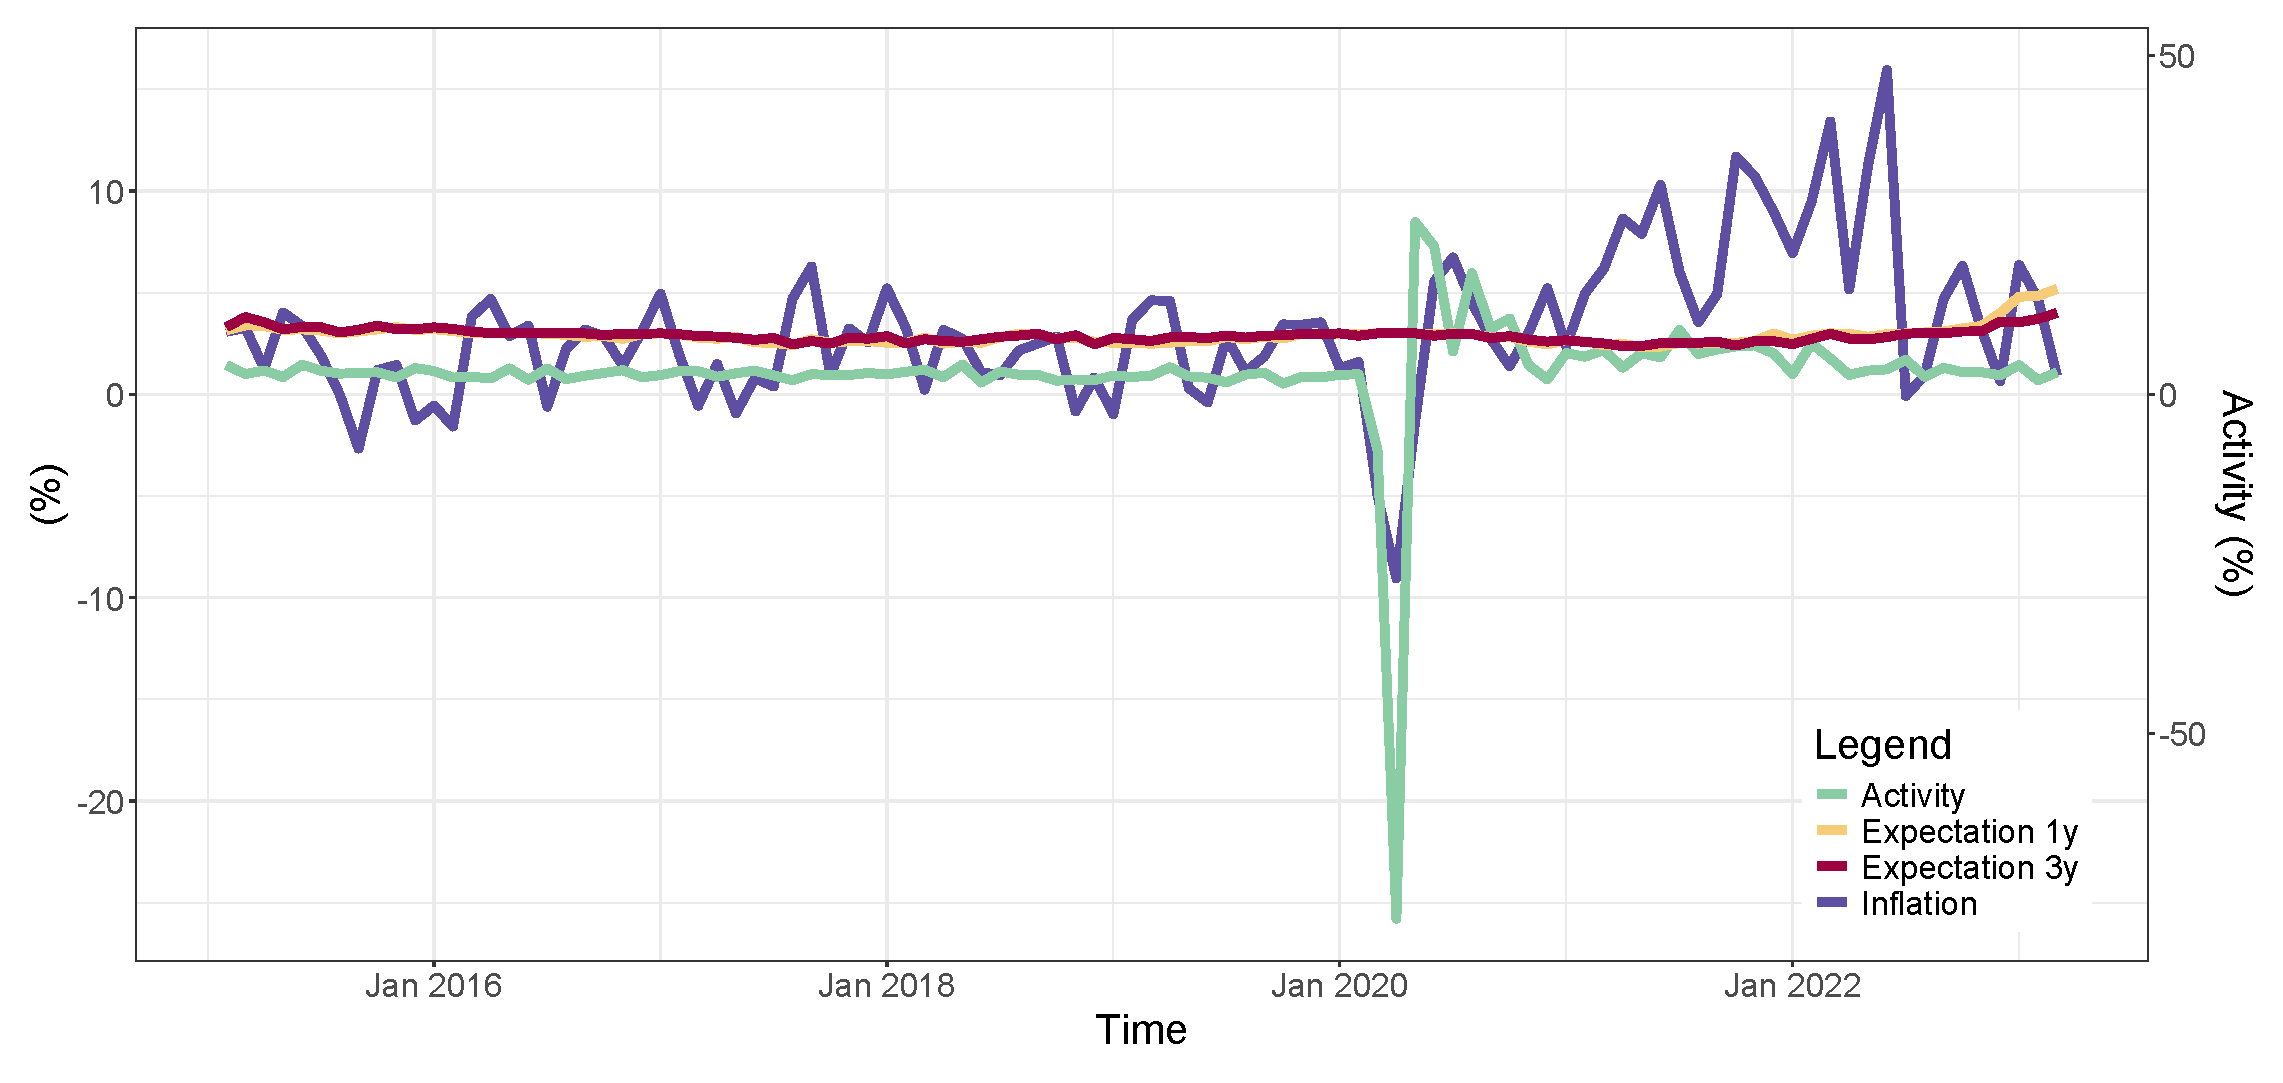
\includegraphics[width=1\linewidth]{figures/all_data.eps}
	\caption{Macroeconomic time series}
	\label{fig:alldata}
	\floatfoot{Note: `Activity' refers to the `Coincident Economic Activity Index for the United States', monthly, seasonally adjusted at annual rates. `Expectation 1y' and `Expectation 3y' refers to `New York Fed: Median 1- and 3-year ahead expected inflation rate', monthly, not seasonally adjusted. `Inflation' refers to `Consumer Price Index for All Urban Consumers: All Items in U.S. City Average', monthly, seasonally adjusted at annual rates. Source: \url{https://fred.stlouisfed.org/} and \url{https://www.newyorkfed.org/microeconomics/sce.html}}
\end{figure}

For the investigation, we use a subset of news content taken from the full corpus, filtered by keywords such as ''inflation'' for the period January 2018 to January 2023 to cover the recent inflation period. Further, the period is limited to five years due to the constrained timeliness of the survey-based measured inflation narratives in \cite{Andre.2023} and filtered by subject codes to select only relevant news sources. This amounts to a corpus of 159,440 documents. Prior to the analysis, further transformations and preprocessing steps are applied to the selected corpus, which are common when working with bag-of-words methods \citep{grimmer.2022}, e.g. lemmatization, stop words removal, constructing a document-feature matrix (see description in section \ref{subsec:DataPrep}).

Second, for the time series analysis we use a macroeconomic time series on CPI inflation (U.S. Bureau of Labor Statistics), inflation expectations (Median survey-based inflation expectations of US households one and three years ahead, New York Fed Survey) and economic activity (Coincident Economic Activity Index (CEI), Federal Reserve of Philadelphia) on a monthly basis (see figure \ref{fig:alldata}). 

CPI inflation and the economic activity index are seasonally adjusted at annual rates, while the inflation expectations are not seasonally adjusted. Moreover, as figure \ref{fig:alldata} shows, the economic activity time series contains several outliers, caused by the first Covid-19 lockdown in 2020. This may introduce a bias tp our estimations. Therefore, we treat these outliers with a dummy variable after they have been detected with the \textsf{tsoutlier()} function as implemented in \cite{forecast.2022}.

%\begin{tcolorbox}[enhanced,breakable,
%	colback=blue!5!white,colframe=blue!75!black,
%	title=To-Do]
%	
%	\begin{itemize}
%		\item Add and reference a table with all data in Appendix?
%	%	\item Document all data transformations! Year over Year on annual base??? Dlog?
%		\item Document filtering and preprocessing steps in Appendix
%	%	\item Create graphs for macroeconomic data series, same style as figure \ref{fig:inflexpect}???
%	\end{itemize}
%	
%\end{tcolorbox}

%\todo[inline]{Add and reference a table in Appendix, }

\subsection{Methods}\label{subsec:methods}

\subsubsection{Semi-supervised Keyword-assisted Topic Model (\textsf{\textbf{keyATM}})}

\cite{Eshima.2023} proposed the \textsf{keyATM} model as a semi-supervised alternative to the benchmark latent dirichlet allocation (LDA) topic model \citep{blei.2003}. They argue: ''[u]nfortunately, although topic models can \textit{explore} themes of a corpus [...], they do not necessarily \textit{measure} specific concepts of substantive interest.'' \citep[1]{Eshima.2023}. Furthermore, benchmark LDA topic models -as an unsupervised method- suffer from the post-hoc interpretability problem \citep{BoydGraber.etal.2014}.

The semi-supervised approach introduced by \cite{Eshima.2023} enables researchers to label topics by specifying keywords before fitting the model. The authors describe it as a ''semi-supervised topic model that combines a small amount of data with a large amount of unlabelled data.''\citep[2]{Eshima.2023}. The baseline \textsf{keyATM} is visualized as a plate representation in figure \ref{graph:basekeyatm} in the Online Appendix. %The proposed model is based on previous work by \cite{Jagarlamudi.etal.2012} but comes with several improvements: %First, \textsf{keyATM} can have non-keyword topics besides keyword topics. This leaves room for further exploration of the corpus. Second, the \textsf{keyATM} model can be extended with meta-information. \citep[3]{Eshima.2023}. 

Specifically, the corpus has $D$ documents and each document has $N_d$ words. $w_{di}$ stands for the $i^{th}$ word in the $d^{th}$ document. The model formulation of \textsf{keyATM} considers two types of topics: keyword topics ($\tilde{K}$) and non-keyword topics ($K$). For each keyword topic $k$ the researcher has to specify a set $L_k$ of keywords. The model is flexible enough to allow keywords to be assigned to different keyword topics simultaneously. The data generation process is modeled in such a way that at first, a latent topic variable $z_{di}$ is sampled from the topic distribution of the document $\theta_d$. If the sampled topic belongs to the non-keyword group, then the word is drawn from the corresponding word distribution of the topic ($\phi_k$). If the topic belongs to the keyword group, a Bernoulli random variable $s_{di}$ is drawn with probability $\pi_k$. This serves as an indicator variable to determine whether the word should be drawn from a set of keywords based on the probability vector $\tilde{\phi}_{k}$ or from the standard topic-word distribution $\phi$. As the estimation is based on standard Bayesian approaches, $\eta, \beta, \gamma, \tilde{\beta}$ indicate priors (see \citet[4 f.]{Eshima.2023} for a more detailed exposition).

Since the model is now based on a mixture of distributions, one with positive probabilities only for keywords on the keyword list and one with positive probabilities for all words, this implies greater prior means for the frequency of the predefined keywords than for the non-keywords in a given topic. As a result, the method is encouraged to give greater importance to keywords \textit{prior} to estimation, but to learn the exact degree of importance from the data. Thus, researchers introduce \textit{a priori} qualitative information into the estimation process of the topic model. 

For this paper we make use of specific variant of the \textsf{keyATM}, namely the \textsf{dynamic keyATM} \citep[22 ff.]{Eshima.2020}. Figure \ref{graph:dynamickeyatm} in the Online Appendix provides a plate representation of the model. As shown in the plate representation, the baseline \textsf{keyATM} is now extended by a hidden Markov model (HMM) with $R$ states where $h_{t[d]}$ denotes the latent state of document $d$ for time $t$. The transition probability matrix of the HMM is sparse, allowing only a one-step forward transition (to simplify the estimation). The \textsf{dynamic keyATM} allows the topic proportion $\theta_d$ to evolve over time by letting $\alpha$ vary across the different latent states. The authors argue that ''(m)odeling $\alpha$ instead of $\theta_d$ makes (the model) less sensitive to short-term temporal variation''. 

For the selection of the pre-specified keywords, we follow the approach of \cite{Eshima.2023} and guide our selection of keywords by the definition and example quotes by the survey study of \cite{Andre.2023}. Moreover, we take into account their results from a penalized logistic regression, which predicts whether or not a DAG factor was manually assigned to a response based on the text data. Finally, we conducted word embeddings of these keywords to optimize our selection. Accordingly, we applied an unsupervised learning algorithm for obtaining vector representations for words called GloVe by using the R Package \textsf{text2vec} \citep{text2vec.2022}. In table \ref{table:narratives}, all prior-selected keywords are listed, additionally with explanations coming from \cite{Andre.2023}. In contrast to their definitions, we use less restrictive definitions due to methodological limitations of the bag-of-words approach, which prevent us from further narrowing them down. Therefore, we treat government mismanagement as ''politics", and the price-gouging narrative as ''profits''. The pent-up demand narrative is excluded due to methodological challenges in distinguishing it from the demand (residual) narrative. Additionally, we do not consider the base effect and inflation expectations narratives, as they do not appear in the households' sample in the original study.

\subsubsection{Latent Semantic Scaling}

Our semi-supervised topic model approach allows us to quantify the prevalence of stories about the potential causes of inflation. To measure a narrative, it is important to identify the direction of its argument, e.g., whether monetary policy is causing rising or falling inflation. Both narratives may exist. Thus, it is essential to distinguish between arguments attributing the different factors to either rising or falling inflation rates. In a way, we follow the idea of ''tone-adjusted time series'' by \citep{Larsen.2019}. To ensure a distinction, simple n-gram prefiltering could be applied, utilizing n-grams such as "rising inflation" or "rising prices". This, however, would only ensure that rising inflation rates are discussed at least once in each document. A more nuanced and accurate measurement of the argument is needed. Therefore, we apply the recently proposed semi-supervised document scaling technique ''Latent Semantic Scaling'' (\textsf{LSS},  \cite{Watanabe.2021}) which is based on a word embedding approach. This allows us to develop a content-related polarity dictionary to indicate if a document is mainly about falling or rising inflation rates. 

\begin{table}[H]
	\centering
	%\scriptsize
	\begin{tabular}{l|l|l}
		\toprule
		Classification 	& ''Positive'' (= increasing) 		& ''Negative'' (= decreasing)\\
		\midrule
						& accelerate 	& decline  \\
						& acceleration  & decrease \\
						& elevate 		& deflation \\
						& high			& fall \\
						& increase		& low \\
						& persist		& lower\\
						& persistent	& reduce\\
						& pressure		& persistent\\
						& rise			& reduction\\
						& surge			& weak\\
		\bottomrule
	\end{tabular}
	\caption{Seed words for LSS initialization}\label{table:seed_words}
\end{table}


\begin{table}
	\caption{Narratives, explanations, and keywords}\label{table:narratives}
	\smallbreak
	\begin{scriptsize}
		\begin{tabular}[htp]{p{3.5cm}|p{5cm}|p{5cm}}		
			\textbf{Category}        & \textbf{Explanation}                                                                                                                                                                            & \textbf{Keywords}                                                                                                                           \\ \toprule 
			\textbf{Demand}          &                                                                                                                                                                                                 &                                                                                                                                             \\ \hline \\[0.02cm]
			Government Spending      & Increases in government spending (e.g., stimulus payments)                                                                                                                                               & infrastructure, agreement, biden, spending, deficit, bipartisan, package                                                                      \\ \\[0.02cm]
			Monetary Policy          & Loose monetary policy by the Federal Reserve                                                                                                                                                   & fed, quantitative, easing, loose, monetary, interest                                                                                        \\ \\[0.02cm]
			Pent-up Demand           & Reopening of the economy and the associated higher incomes, new spending opportunities, and optimism about the future & demand, surge, activity, recover, pandemic \\ \\[0.02cm]
			Demand Shift             & Shift of demand across sectors   (particularly increases in durables). 
			& change, consumer, good, durable, trend, service, shift, vehicle,                                                                                 \\ 
			&                                                                                                                                                                                                 &                                                                                                                                             \\
			\textbf{Supply}          &                                                                                                                                                                                                 &                                                                                                                                             \\ \midrule \\[0.02cm]
			Supply chain issues      & Disruption of global supply chains                                                                                                                                                             & supply, supplier, chain, producer, bottleneck                                                      \\ \\[0.02cm]
			Labor shortage           & Shortage of workers, e.g., due   to some workers dropping out of the labor force, and higher wage costs  & worker, employment, labor, wage, workforce, labour, job, strike, union, hire            \\ \\[0.02cm]
			Energy crisis            &  The global energy crisis,   leading to shortages of, e.g., oil and natural gas and higher energy prices 
			& crude, gas, gasoline, oil, fuel                                                                                                             \\ 
			&                                                                                                                                                                                                 &                                                                                                                                             \\
			\textbf{Miscellaneous}   &                                                                                                                                                                                                 &                                                                                                                                             \\ \hline \\[0.02cm]
			Pandemic                 & The COVID-19 pandemic, the   global pandemic recession, lockdowns, and other policy measures                                                    & pandemic, covid-19, virus, coronavirus, infection, outbreak, case                           \\ \\[0.07cm]
			Politics & Policy failure, mismanagement by   policymakers, policymakers are blamed                                                            & part, republican, trump, congress, senate, president, biden, democrats, government\\ \\[0.02cm]
			Russia-Ukraine war       & The Russian invasion of Ukraine,   the international economic, political, and military response                                               & russia, war, ukraine, invasion, moscow, putin, military                           \\ \\[0.02cm]
			Government debt          & High level of government   debt                                                                                                                                                                & debt, public, national, federal, deficit, borrowing, government, balance                                                                   \\ \\[0.02cm]
			Tax increases            & Tax increases, such as VAT   hikes                                                                                                                                                             & tax, raise, reform, legislation, overhaul, reduction\\ \\[0.02cm]
			Profits            & Greedy companies exploiting opportunities to increase profits, companies trying to make up for the money they lost during the pandemic & margin, corporate, profitability, profit, growth      \\ \\[0.02cm] \bottomrule                                                                  
		\end{tabular}
	\end{scriptsize}
\end{table}



\normalsize

Sentiment or polarity analyses are traditionally conducted by means of a dictionary approach \citep[180]{grimmer.2022}. Consequently, the major challenge is to select a domain specific dictionary or construct an own dictionary. To our knowledge, the former does not exist for the context of inflation, while the latter would be extremely time consuming. Then again, supervised machine learning methods could by applied to predict the sentiment of each document. This involves manual coding of a sufficiently large corpus, to insure reappearance of words in the training and test set, which again is time and cost intensive \citep[84]{Watanabe.2021}. In contrast, \textsf{LSS} allows us to construct our own polarity dictionary using seed and target words. Based on the proximity to a selection of seed words for each semantic dimension, polarity scores of words are computed. To estimate the semantic closeness of words, LSS recalls on singular value decomposition (SVD) of a document-feature matrix. The selected seed words are listed in table \ref{table:seed_words}. For further refinement of the polarity analysis on inflation, relevant target words are selected. Therefore, we opt for glob pattern ''infla*'' and ''price*''. Following our selection, the LSS method generates a collection of statistically significant words that occur within a window of five words around the target words. Polarity scores of words are computed as follows:

\begin{equation}
	g_f=\frac{1}{|s|}\sum_{s\in S}cos(v_s, v_f)P_s
\end{equation}


where $g_f$ are words, $s$ seed words, $p_s$ user-provided polarity of seed words, and $cos(v_s, v_f)$ the cosine similarity between the seed word vector and the word vector associated with the word f \citep[86]{Watanabe.2021}. Subsequently, the polarity scores of the documents are predicted by weighting word polarity scores by their frequency in the document: 

\begin{equation}
	y=\frac{1}{N}\sum_{f\in F}g_fh_f
\end{equation}

where $h_f$ is the frequency of words and $N$ the total number of words in the model. The documents' scores are symmetrically distributed around the mean ($\mu = 0$), and rescaled by standard deviation ($\sigma = 0$). In our case, a negative score indicates that the document is mainly about falling inflation rates, while a positive score indicates that the document is mainly about rising inflation rates. For our further analysis, we constructed narrative indices based on the document scores and the topic prevalence time series from our \textsf{keyATM} analysis. For this, we multiply the topics' proportions on the document level with the document polarity score. Finally, we aggregated our index on monthly level. 

\subsubsection{Granger Causality Tests}

In order to study the macroeconomic dynamics of our narratives, we first conducted a series of Granger causality test using our constructed narrative indices as a proxy for the narratives' virality. This allows us to study the predictive power of our narrative time series on macroeconomic variables (inflation expectations, CPI inflation, economic activity) and test their (weak) exogeneity. The Granger causality tests are constructed as multivariate tests in a vector autoregressive model (VAR) setting. The hypotheses of no Granger causality is tested by means of F test for joint significance. We follow the argument of \cite{Luetkepohl.2005}, that an $\chi^2$-distribution is often a poor approximation when working with a small sample size as ours. For our purpose we again consider five macroeconomic variables: the households' 1- and 3-year inflation expectations, the CPI inflation, the economic activity. The Granger causality statistics are used to examine whether the lagged values of one variable help to predict another one. In a more general sense we say that variable z Granger causes y if:

\begin{equation}
	\E(y_t|I_{t-1}) \neq \E(y_t|J_{t-1})
\end{equation}

\noindent Here, the vector $I_{t-1}$ contains past values of y and z, while the vector $J_{t-1}$ only contains past information on y \citep{wooldridge.2013}. Granger causality thus follows the idea that a cause cannot succeed the effect \citep[41]{Luetkepohl.2005}. 

\subsubsection{Local Projections}

To further investigate the effects of increasing narrative diffusion at the macroeconomic level, we resort to dynamic time series models and, in particular, impulse response functions (IRF). Classical tools are VARs \citep{Sims.1980}. This method, however, has some drawbacks: it is prone to mis-specification, difficult to apply to non-linear cases, and usually necessitates a relatively long lag length to ensure proper calculation \citep[161]{Jorda.2005}. The latter is of particular importance for the present study, since a rather short observation period is used. We therefore decided to estimate the dynamic response sequences on the basis of ''local projections'' (LP) method \citep{Jorda.2005}. \cite{Plagborg.2021} recently proved that under reasonable assumptions, VAR and LP estimate the same IRFs.

The basic idea of LP is to compare a conditional forecast of an event using currently available information at the time of a shock to a forecast without the shock \citep[163]{Jorda.2005}:
\begin{equation}
	IR(t,s,\bm{d}_i) = \E(\bm{y}_{t+s}|\bm{v_t} = \bm{d}_i;\bm{X}_t)-\E(\bm{y}_{t+s}|\bm{v}_t=O;\bm{X}_t), \; s = 0,1,2,...,S
\end{equation}
\noindent The operator $\E(.|.)$ denotes the best predictor of the mean square deviation, $X_t \equiv (y_{t-1},y_{t-2}...)$ and $d_i$ is a vector containing all relevant shocks. Unlike in the VAR method, the LP method estimates the impulse response using least squares regressions for each time horizon $s$ with $s=0,1,2,...S$ \citep[423]{Adaemmer.2019}:

\begin{equation}\label{eq:lp}
	\bm{y}_{t+s}=\bm{\alpha}^s+\bm{\beta}_1^{s+1}y_{t-1}+\bm{\beta}_2^{s+1}y_{t-2}+...+\bm{\beta}_p^{s+1}y_{t-p}+\bm{u}_{t+s}^s, \; s=0,1,2...,S
\end{equation}

\noindent Here, $\alpha^s$ is a vector of constants and $\beta_i^{s+1}$ are matrices with coefficients for each lag $i$ and forecast horizon $s+1$ \citep[163]{Jorda.2005}. The $\beta$ coefficients derived from the regressions are used to construct the impulse responses. Therefore, the collection of all regressions from equation \ref{eq:lp} are called \textit{Local Projections} \citep[423]{Adaemmer.2019}. The impulse responses of these local linear projections are defined as:

\begin{equation}
	\widehat{IR}(t,s,\bm{d}_i) = \hat{\bm{B}}_{1}^s\bm{d}_i, \; s=0,1,2,...,h
\end{equation}
\noindent where $\hat{\bm{B}}_1^s$ contains the coefficients of the impulse response and $\bm{d}_i$ is the vector of all relevant shocks. 

\subsubsection{Stationarity and De-trending}

The modelling of time series in VAR or ARDL models is typically based on the assumption of weak stationarity \citep[13]{Kirchgaesser.2007}. If this property is not present, there are several options: any long-run relationships that may exist can be taken into account by modelling as an error correction model, or the time series can be transformed into a stationary representation using appropriate transformations. 

Due to the short time series and the simultaneous consideration of unit root tests (see \ref{table:ers} in Online Appendix), we had to choose a trend removal approach. Simple differencing may come at costs, as such an approach may lead to information loss and spurious independence, which could result in insignificant coefficients or downward biased results \citep[201]{Kirchgaesser.2007}. However, modelling the time series at the level only makes sense if the long-term relationships are stable. We have therefore chosen another form of trend adjustment.

As \cite{hamilton.2018, phillips.2021b} have shown, applying the popular HP filter \citep{hodrick.1997} has the potential of causing an inadequate statistical trend removal leading to (worsening) spurious results, especially when the default tuning parameter is used. Several alternatives have been suggested in the literature, including the Hamilton-Filter \citep{hamilton.2018} and a boosted HP-Filter \citep{phillips.2021}. We opt for the latter, because it enables us to achieve stationarity without a loss of observation and its proved robustness with shorter sample sizes \citep{phillips.2021b}. Thus, we report our baseline estimations with trend-cycle filtered time series by means of the boosted HP-Filter. 

For robustness checks, we follow the suggestion of the literature \citep[159]{Kirchgaesser.2007} and provide level and difference estimations in the Online Appendix. Further, sufficient consideration of lags of endogenous variables should help avoid the problem of ''spurious regression'' results. To select the system's lag order, we rely on the Schwarz information criterion (SC) with a maximum of 4 lags.
 


% Here: Analysis section
% !TeX spellcheck = en_US
\section{Empirical Analysis}\label{sec:Analysis}

 In this section, we present our empirical results, starting with a descriptive overview of the measured \textsf{keyATM} topics between 2019 and 2023. Next, we introduce our polarity score, which measures media reports on rising or falling inflation rates based on word embeddings. By integrating our polarity analysis with the results from the \textsf{keyATM}, we derive our final narrative indices. Utilizing these indices, we conduct multivariate Granger causality tests to assess the predictive power of our measured narratives. By disaggregating household expectations, we are able to identify differences based on a range of socio-economic factors. Finally, we employ local projections to study the effect of narrative diffusion on the macroeconomy.

\subsection{Narrative Topics}\label{subsec:atmtopics}

We begin by examining the interpretability of the resulting topics, following the procedure recommended by \citet{Eshima.2023}, and provide an overview of the topic-word distribution. In other words, we highlight terms with high probabilities of topic selection. These terms are visualized in figure \ref{fig:wordclouds} as wordclouds for each of the considered topics. The larger a term appears, the more likely it is to be selected for a respective topic. The wordclouds illustrate the topics' consistency with the underlying narrative concepts. Moreover, multiple pre-selected keywords appear in the vast majority of topics. This presence, along with topic-consistent terms, suggests a successful measurement of the respective concepts. For example, terms like ''unemployment'', ''work'', and ''growth'' are closely related to the labor shortage narrative, while ''bill'', ''biden'', and ''spending'' align with the government spending narrative. Nearly all topics are clearly related to their underlying narratives. The demand shift topic, however, requires additional expert knowledge for a clearer evaluation. Many terms are at least indirectly associated with shifts in demand as a cause of inflation. For instance, terms such as ''sale'', ''expect'', and ''quarter'' are related to sales reports or analyst forecasts, aligning with the narrative since (expected) changes in sales are part of the argument. Additionally, the wordcloud includes terms linked to consumer shifts toward online retailers (e.g., ''Amazon'' and ''online''), full stocks (e.g., ''stock'' and ''store''), or consumer behavior (e.g., ''consumer'' and ''spending''). Based on this reasoning, we conclude that the topic estimation is successful.

Following the discussion on consistency, we consider the development of topic proportions over time. As figure \ref{fig:narr_all} illustrates, there are some major changes present over time. The pandemic topic surge stands out overall. It is marked by a sudden increase that is sustained with elevated shares until the conclusion of 2022. The strong increase in the war topic is also sudden, although of short duration. More generally, proportions start to shift in 2021, when inflation rates began to rise. Significant steady increases are observed for the demand shift, supply chain, energy, and profits topics. Among these, the most notable increases are reported for the supply chain and demand shift topics. Additionally, the government spending and labor shortage topics experience slight increases. However, the latter already starts declining in 2021. We observe more fluctuations for the demand (residual) topic. It is characterized by losses in early 2020 but recovers and gains importance, especially at the end of 2022.

We observe a similar picture in the monetary policy topic. It also declines during the early phase of the pandemic, however, it shows recovery towards the end of the observation period. On the contrary, the debt topic shows a more steady decline. This topic is characterized by only occasional minor increases during the outbreak of the pandemic. The tax topics maintained relatively stable shares throughout the observation period, whereas the politics topic shows more fluctuations. It experiences an increase at the end of 2020, coinciding with the presidential election. Additionally, we observe a slight increase in relative importance towards the end of 2022.

\begin{figure}[H]
	\centering
	\includegraphics[width=0.65\linewidth, angle = 270]{figures/narratives_all.eps}
	\caption{Change of smoothed proportions}
	\label{fig:narr_all}
	\floatfoot{Note: The figure shows the development of the smoothed proportions. To calculate the relative proportions only the topics with pre-specified keywords were considered. To build this plot we employed the \textsf{geom\_stream()} function by \cite{Sjoberg.2021}. We organized the topics by following the code system provided by \cite{Andre.2023}.} 
\end{figure}

To ensure robustness irrespective of the news structure, we provide a subsample comparison \textsf{keyATM} estimation that only includes Wall Street Journal (WSJ) articles, as illustrated in figure \ref{fig:comparision} in the Online Appendix. The WSJ corpus includes approximately 25,500 documents. While most topics exhibit similar trajectories, a few minor differences are observed. On the one hand, smaller volumes for the pandemic and supply chain topics are found in the WSJ corpus. However, a simultaneous trend is present. On the other hand, the politics topic shares are greater with the WSJ corpus. Overall, the topics in the WSJ corpus appear to react more strongly to singular events compared to the baseline corpus, which includes more financial and corporate sources.

\begin{figure}
	\begin{subfigure}{0.32\textwidth}
		\includegraphics[width=0.7\textwidth,angle=270]{figures/wordcloud7.eps}
		\caption{Government spending}
	\end{subfigure}
	\begin{subfigure}{0.32\textwidth}
		\includegraphics[width=0.7\textwidth,angle=270]{figures/wordcloud6.eps}
		\caption{Monetary policy}
	\end{subfigure}
	\begin{subfigure}{0.32\textwidth}
		\includegraphics[width=0.7\textwidth,angle=270]{figures/wordcloud9.eps}
		\caption{Demand shift}
	\end{subfigure}
	\begin{subfigure}{0.32\textwidth}
		\includegraphics[width=0.7\textwidth,angle=270]{figures/wordcloud8.eps}
		\caption{Demand (residual)}
	\end{subfigure}
	\begin{subfigure}{0.32\textwidth}
		\includegraphics[width=0.7\textwidth,angle=270]{figures/wordcloud5.eps}
		\caption{Supply chain}
	\end{subfigure}
	\begin{subfigure}{0.32\textwidth}
		\includegraphics[width=0.7\textwidth,angle=270]{figures/wordcloud1.eps}
		\caption{Energy}
	\end{subfigure}
	\begin{subfigure}{0.32\textwidth}
		\includegraphics[width=0.7\textwidth,angle=270]{figures/wordcloud4.eps}
		\caption{Labor shortage}
	\end{subfigure}
	\begin{subfigure}{0.32\textwidth}
		\includegraphics[width=0.7\textwidth,angle=270]{figures/wordcloud14.eps}
		\caption{Supply (residual)}
	\end{subfigure}
	\begin{subfigure}{0.32\textwidth}
		\includegraphics[width=0.7\textwidth,angle=270]{figures/wordcloud3.eps}
		\caption{Pandemic}
	\end{subfigure}
	\begin{subfigure}{0.32\textwidth}
		\includegraphics[width=0.7\textwidth,angle=270]{figures/wordcloud2.eps}
		\caption{War}
	\end{subfigure}
	\begin{subfigure}{0.32\textwidth}
		\includegraphics[width=0.7\textwidth,angle=270]{figures/wordcloud11.eps}
		\caption{Politics}
	\end{subfigure}
	\begin{subfigure}{0.32\textwidth}
		\includegraphics[width=0.7\textwidth,angle=270]{figures/wordcloud12.eps}
		\caption{Government Debt}
	\end{subfigure}
	\begin{subfigure}{0.32\textwidth}
		\includegraphics[width=0.7\textwidth,angle=270]{figures/wordcloud13.eps}
		\caption{Taxes}
	\end{subfigure}
	\begin{subfigure}{0.32\textwidth}
		\includegraphics[width=0.7\textwidth,angle=270]{figures/wordcloud10.eps}
		\caption{Profits}
	\end{subfigure}

	\caption{Wordclouds of \textsf{keyATM} keyword topics}
	\label{fig:wordclouds}
\end{figure}
\newpage

  
  
 
\subsection{Polarity-adjusted Narrative Time Series}
So far, using a \textsf{keyATM} model enables us to measure reports on various causes of inflation. However, a key challenge lies in discerning the directions of these arguments, significantly impacting the subsequent econometric time series analysis. As detailed in \ref{subsec:methods}, we address this issue by employing \textsf{LSS} to identify whether a document is mainly about (expected) rising or falling inflation rates. \cite{Ellen.2022} previously highlighted this methodological challenge. However, by applying a simple dictionary method, their approach falls short ``[...] to identify the difference in tonality for specific narratives, for example, with respect to inflation, and not only the overall contribution'' \citep[1533]{Ellen.2022}. In contrast, our approach enhances this methodology by employing semantic scaling to create a case-specific dictionary that identifies the narrative components’ tonality. Subsequently, we construct an index for each narrative by multiplying the sentiment score of a document by the relative proportions of the \textsf{keyATM} topics in each document. This is concluded by aggregating our data on monthly-level, resulting in the final indices of the narratives.

\begin{figure}[H]
	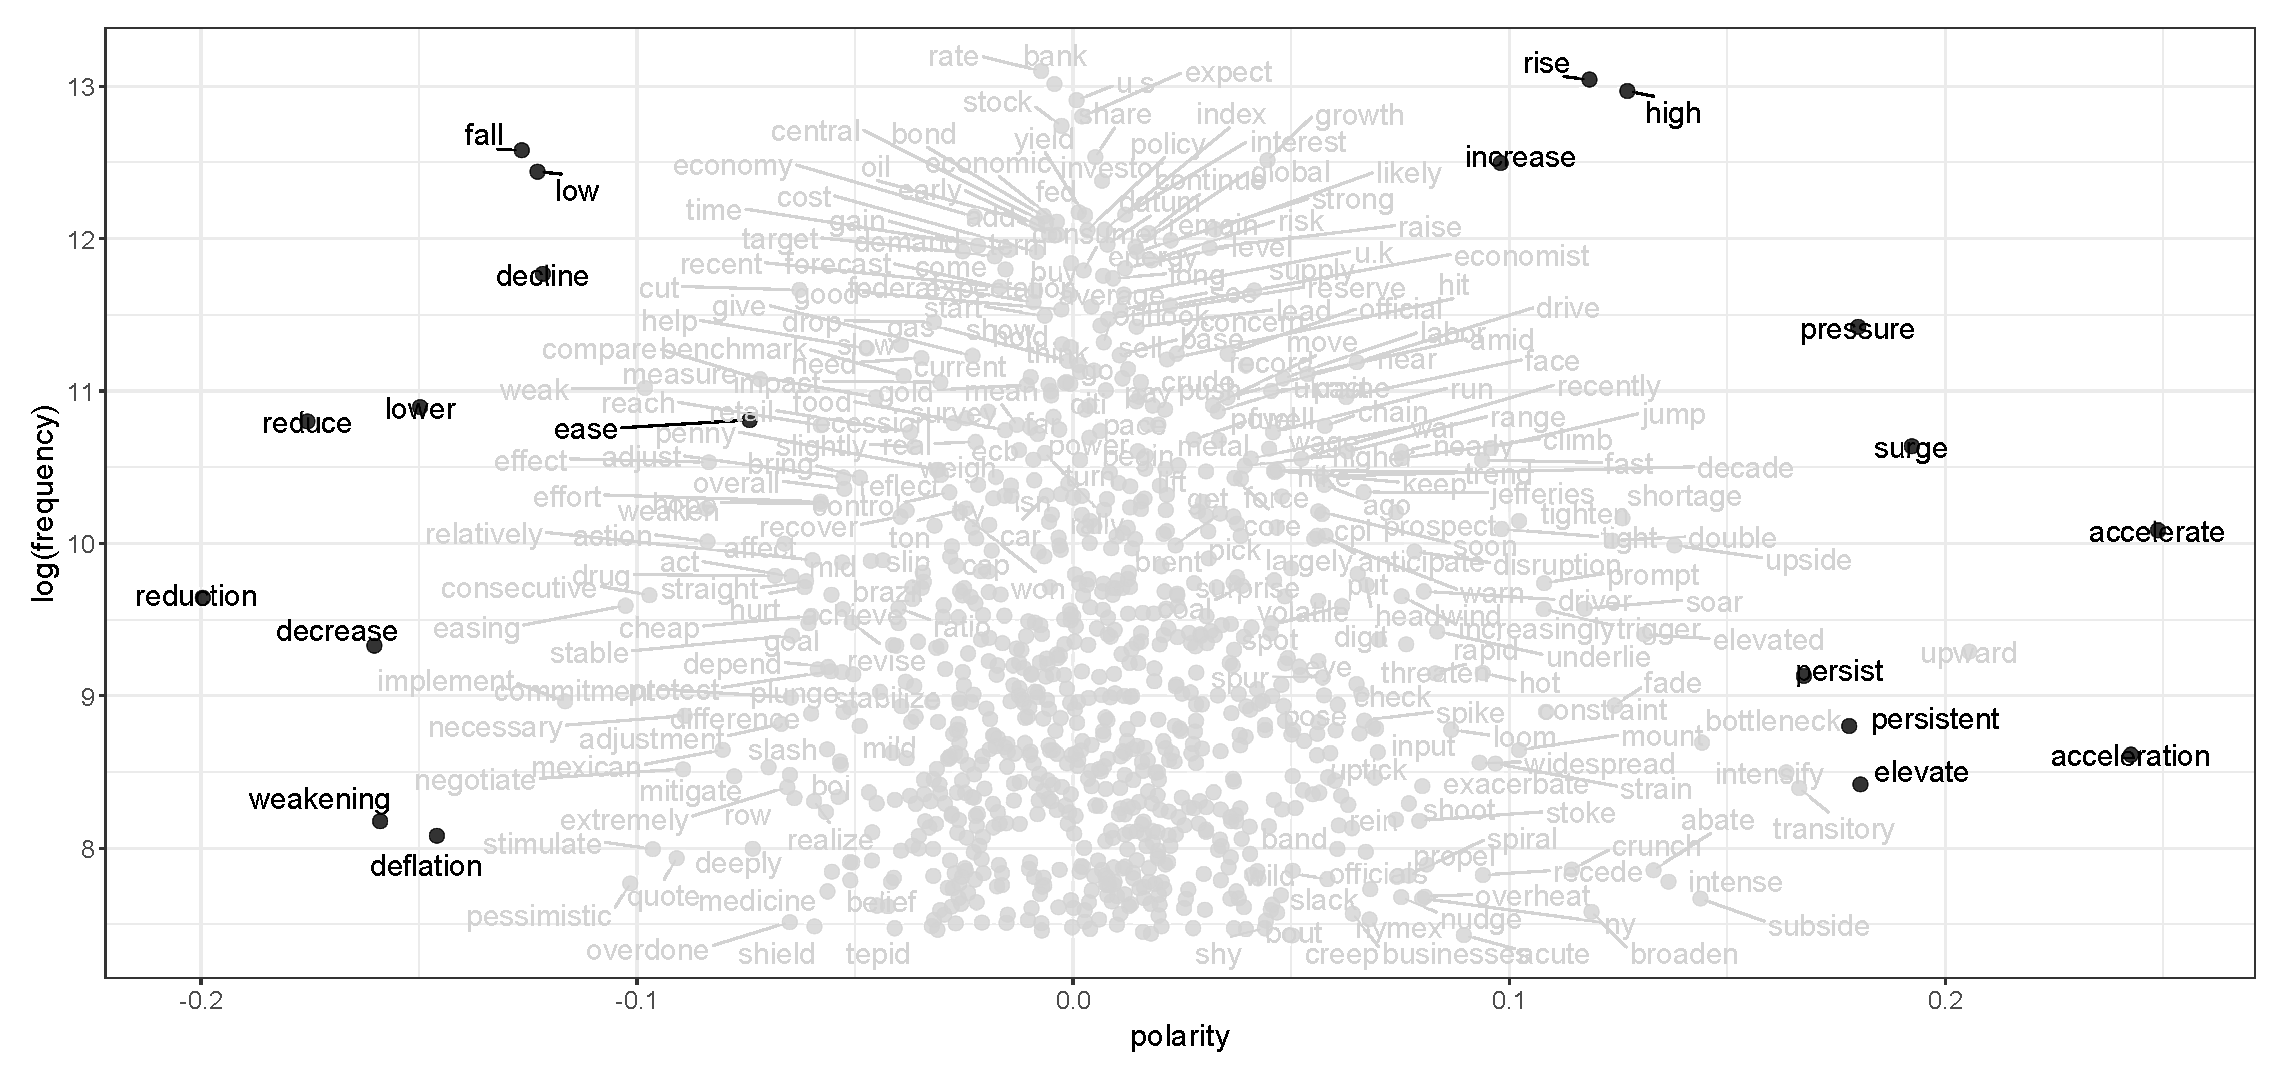
\includegraphics[width=1\textwidth]{figures/lss_words.eps}
	\caption{Polarity of words (seed words highlighted)}
	\label{fig:polarity}
	\floatfoot{Note: The figure shows the polarity scores for all statistically significant words around the target words ``infla*'' and ``price*''. To compute the polarity score, the semantic closeness towards pre-selected seed words are considered. To facilitate orientation, the utilized seed words are highlighted.} 
\end{figure}

 To evaluate the results of \textsf{LSS}, we plot the polarity scores constructed from our chosen seed words in figure \ref{fig:polarity}. The pre-selected seed words are highlighted in the figure. Those terms associated with falling inflation rates, such as ``deflation'', ``negative'', or ``downturn'' possess a negative polarity score. In contrast, terms like ‘intensify,’ ‘tight,’ or ‘shortage’ have a positive score. Additionally, the majority of words is located around the midpoint of the polarity score line. This is reasonable because most words are not implicitly associated with changing inflation rates. Examples, such as "affect," "likelihood," and "expect," share the characteristic of not being explicitly aligned with discussions about increasing or decreasing inflation rates. Thus, this observed neutrality can be interpreted as further validation for how accurate the estimation is. 
 
By weighting the polarity scores for each document, as described in \ref{subsec:methods}, we construct an aggregated polarity score at the document level. Figure \ref{fig:sentiment} shows the smoothed polarity score over time. As the plot demonstrates, the polarity score experiences strong fluctuations over the observation period. The figure shows a profound decline in the polarity score since the end of 2018. This trend corresponds with the realized CPI inflation, which began to decrease in mid 2018 and maintained low levels through October 2019. During this period, the US economy experiences a slowdown in growth. This is followed by a brief recovery of the inflation polarity, starting a the end of 2019. While the overall CPI inflation remained relatively low, an upward trend was still evident \footnote{For comparison: U.S. Bureau of Labor Statistics, Consumer Price Index for All Urban Consumers: All Items in U.S. City Average [CPIAUCSL], retrieved from FRED, Federal Reserve Bank of St. Louis; https://fred.stlouisfed.org/series/CPIAUCSL, February 21, 2024.}. Following the first lockdowns, we observe an increase in the polarity score starting in mid-2020. The score turns overall positive in 2021 and remains so until late 2022, peaking in late 2021.

\begin{figure}[H]
	\centering
	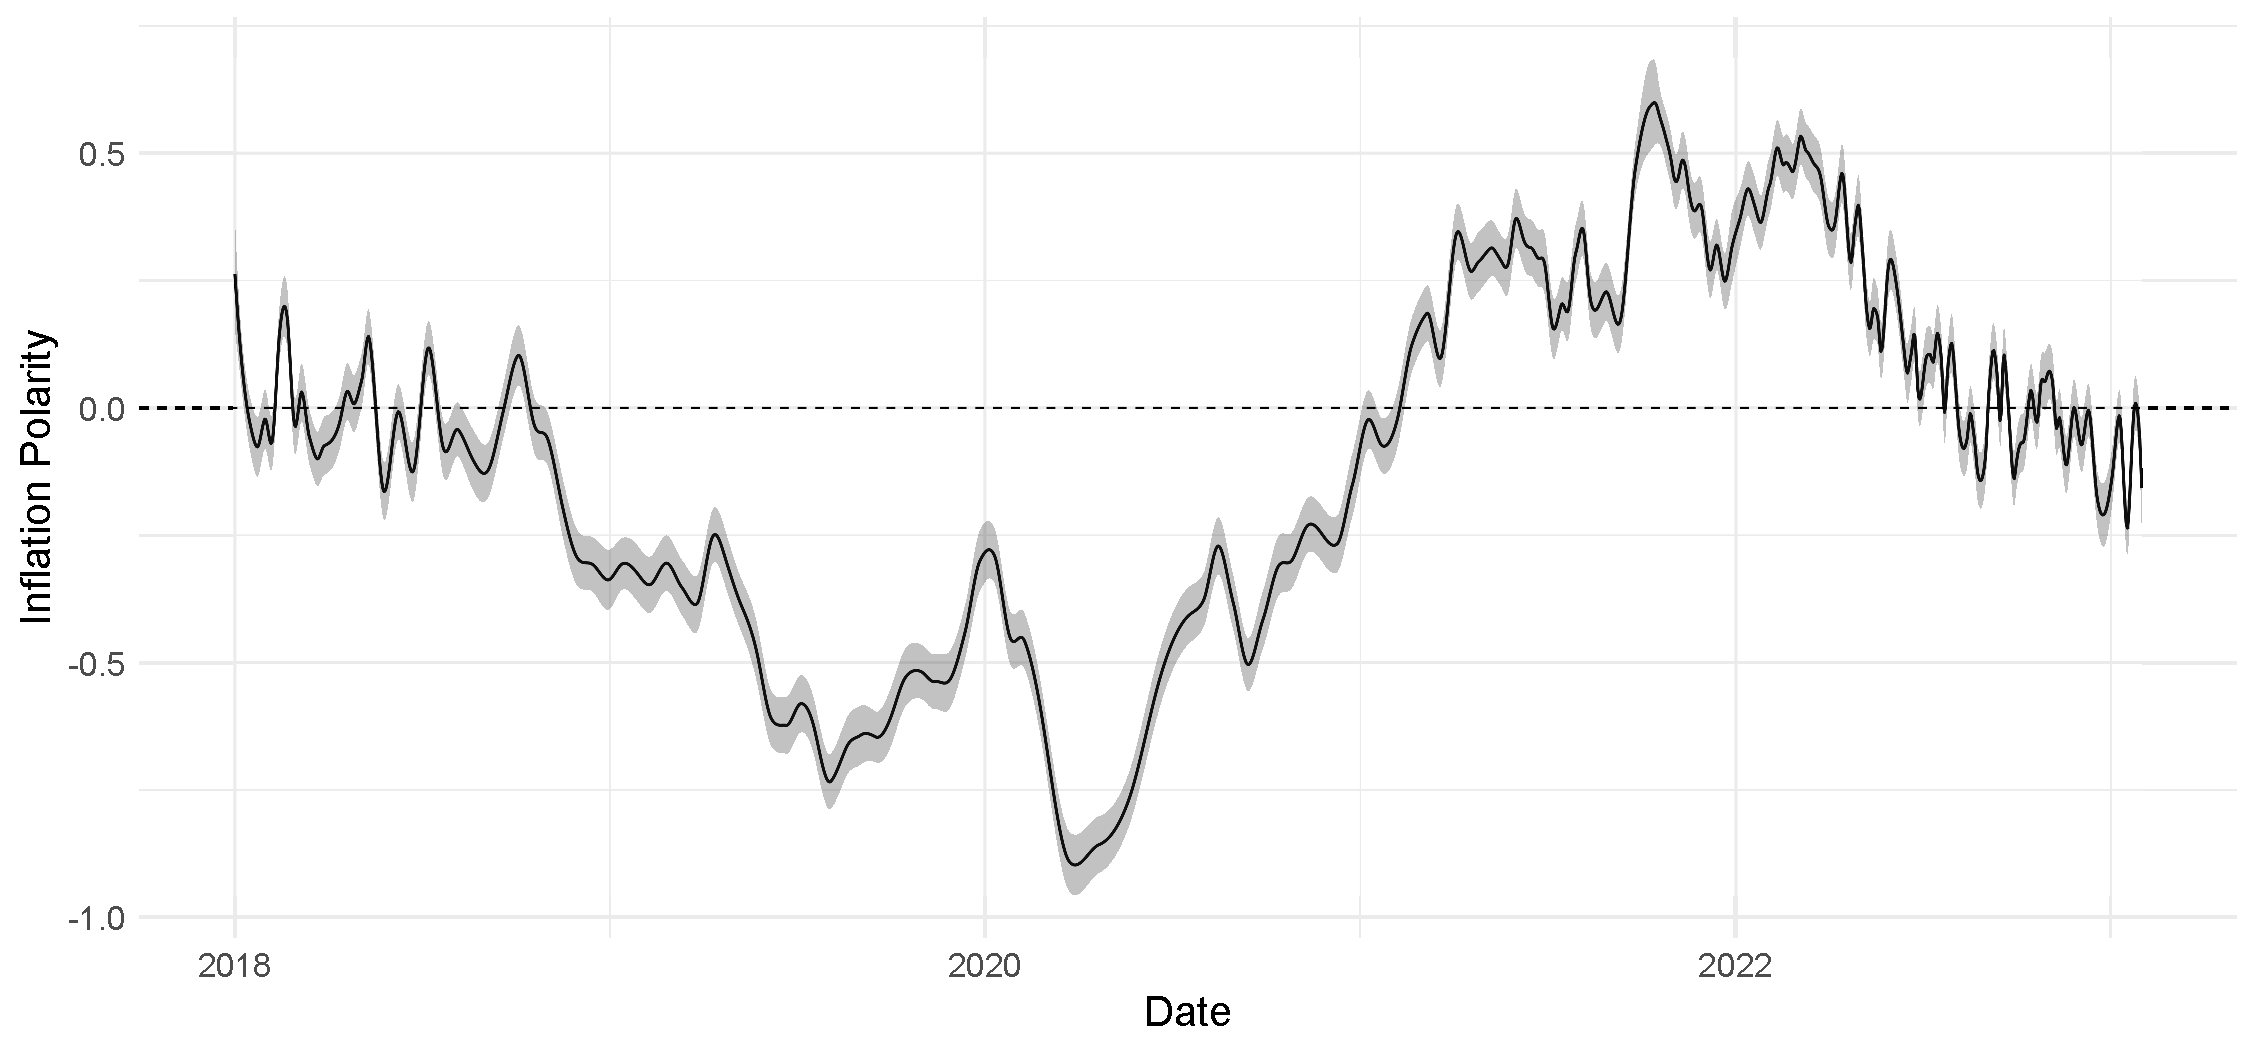
\includegraphics[width=0.95\linewidth]{figures/sentiment.eps}
	\caption{Change of polarity in corpus}
	\label{fig:sentiment}
		\floatfoot{Note: The figure shows the development of the aggregated polarity score computed by \textsf{LSS}. To ensure readability, the time series is smoothed by applying a local polynomial regression \citep{Watanabe.2023} with 95\% confidence intervals.} 
\end{figure}



Lastly, by combining our \textsf{keyATM} and \textsf{LSS} results, we construct the final narrative indices. We begin with the demand narratives, which are visualized in figure \ref{fig:sdemand}. As the figure illustrates, the demand inflation narratives are present during two considered periods: the non-inflationary (pre- and early pandemic) and the inflationary period (particularly since 2021). Until mid-2020, narratives highlighting monetary policy and residual demand factors are particularly prominent. The importance of the monetary policy narrative is exceptionally strong in mid-2019, meaning that a large number of reports about falling inflation rates were discussing aspects of monetary policy. This coincides with the previously discussed fall of the CPI rate under the inflation target. It also marks the first interest rate cut by the Fed in eleven years \citep{fed.2019}. In late 2021, the narrative reaches positive values and gains relative significance in the media coverage about rising inflation rates.
\begin{figure}[H]
	\begin{subfigure}[b]{0.95\textwidth}
		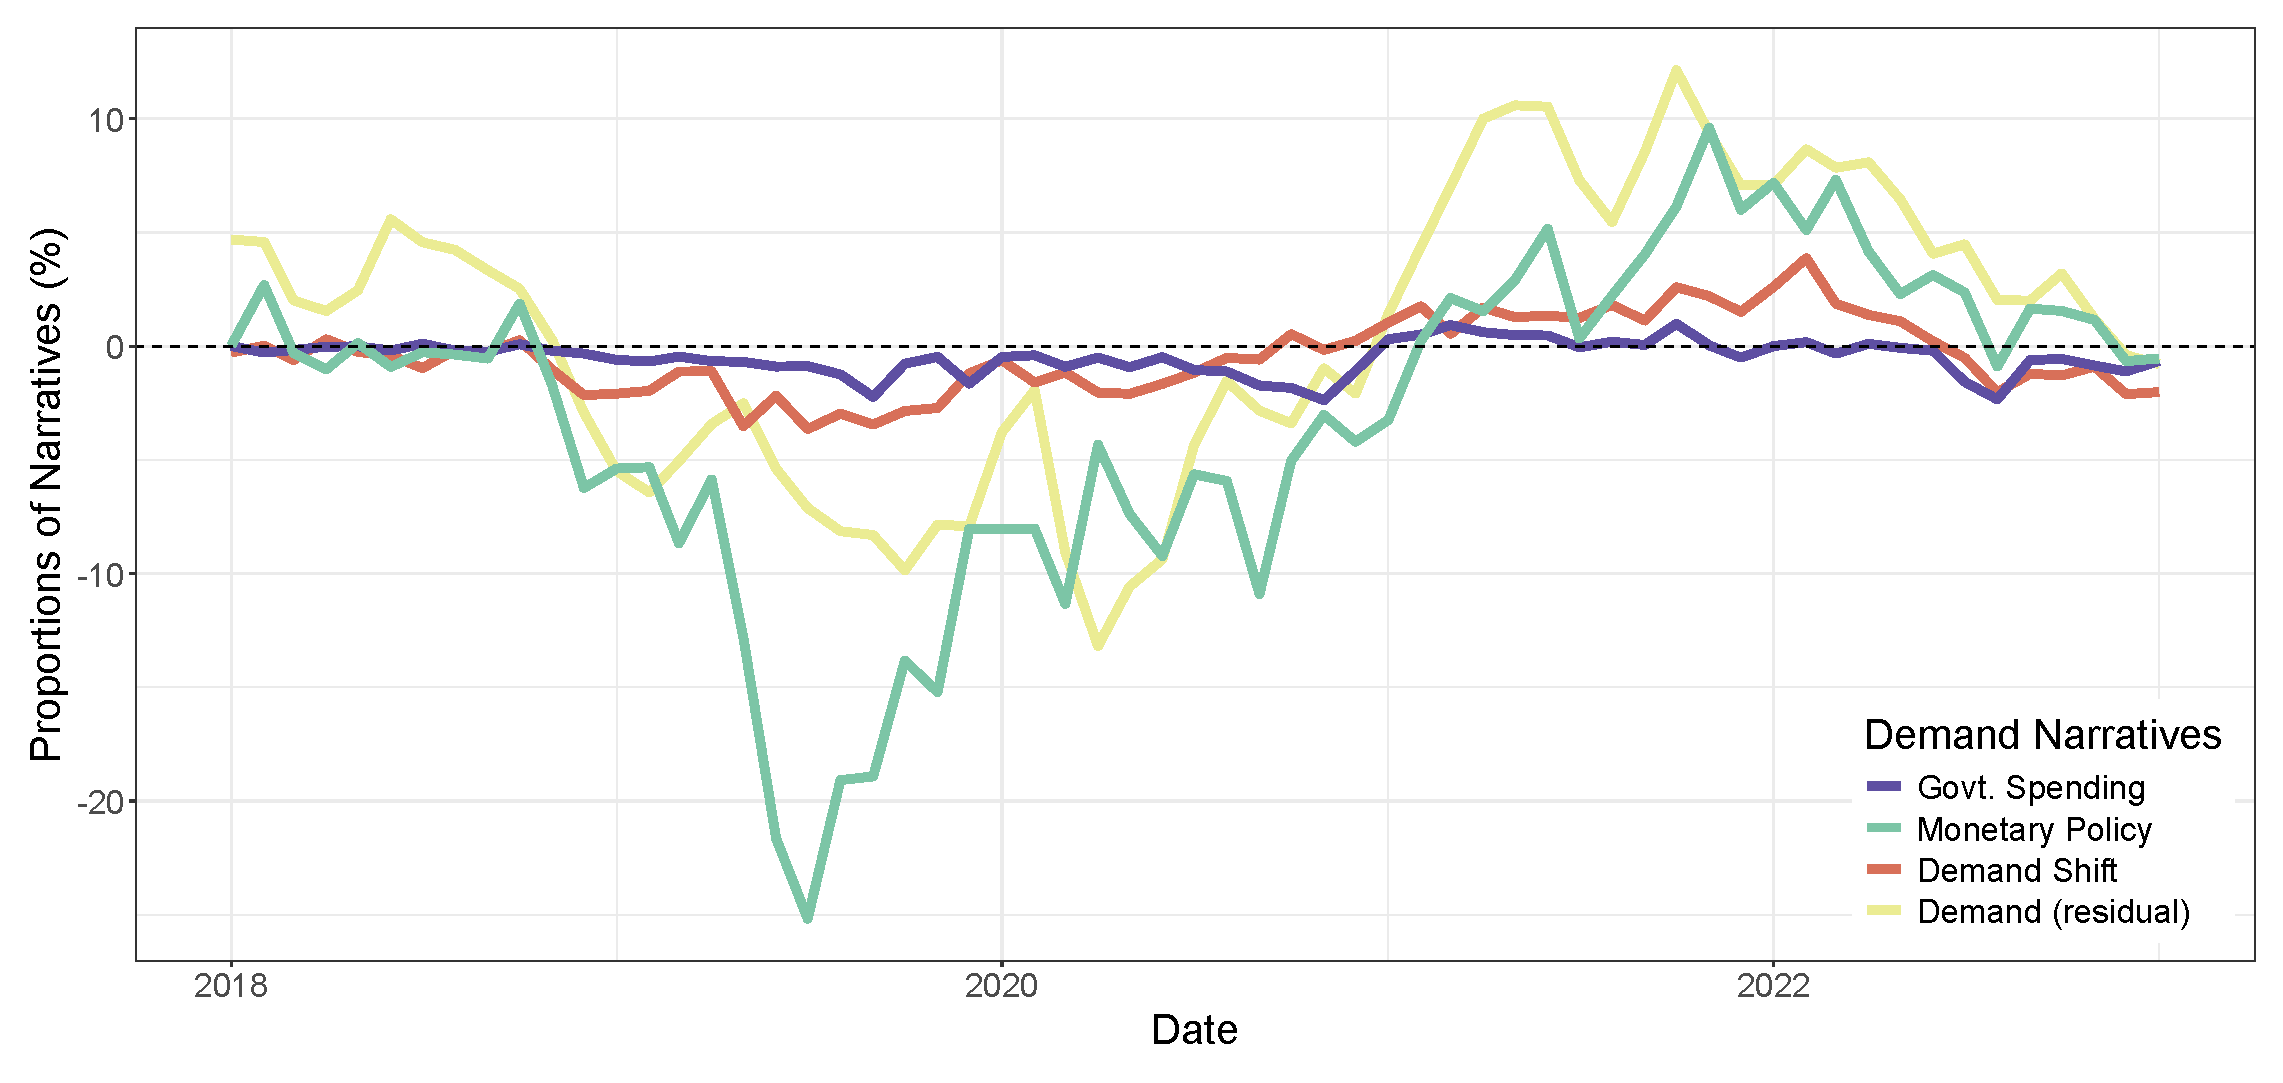
\includegraphics[width=\textwidth]{figures/plot_sdemand.eps}
		\caption{Indices of demand narratives}
		\label{fig:sdemand}
	\end{subfigure}
	\hfill
	\begin{subfigure}[b]{0.95\textwidth}
		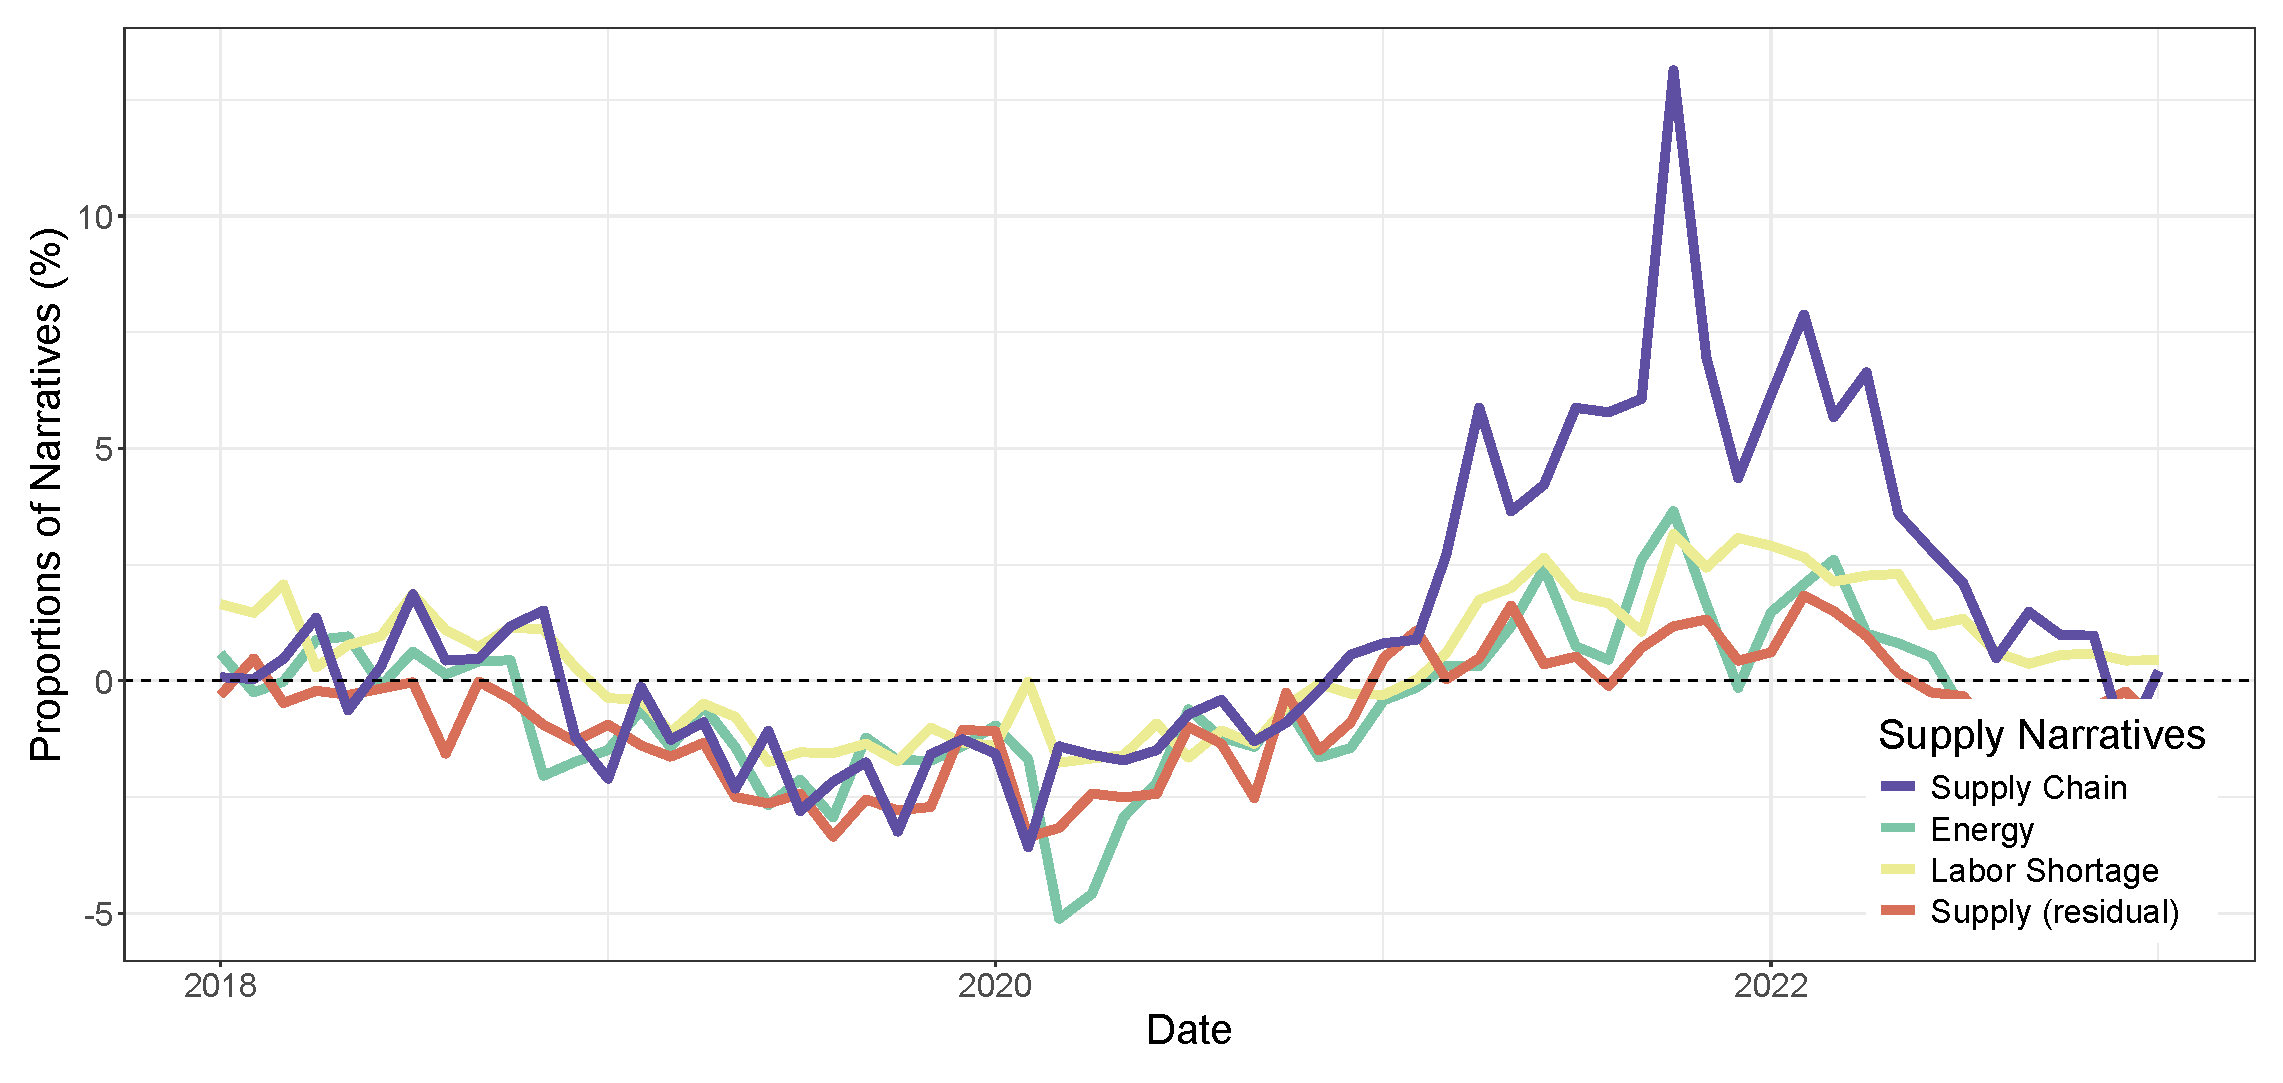
\includegraphics[width=\textwidth]{figures/plot_ssupply.eps}
		\caption{Indices of supply narratives}
		\label{fig:ssupply}
	\end{subfigure}
	\hfill
	\begin{subfigure}[b]{0.95\textwidth}
		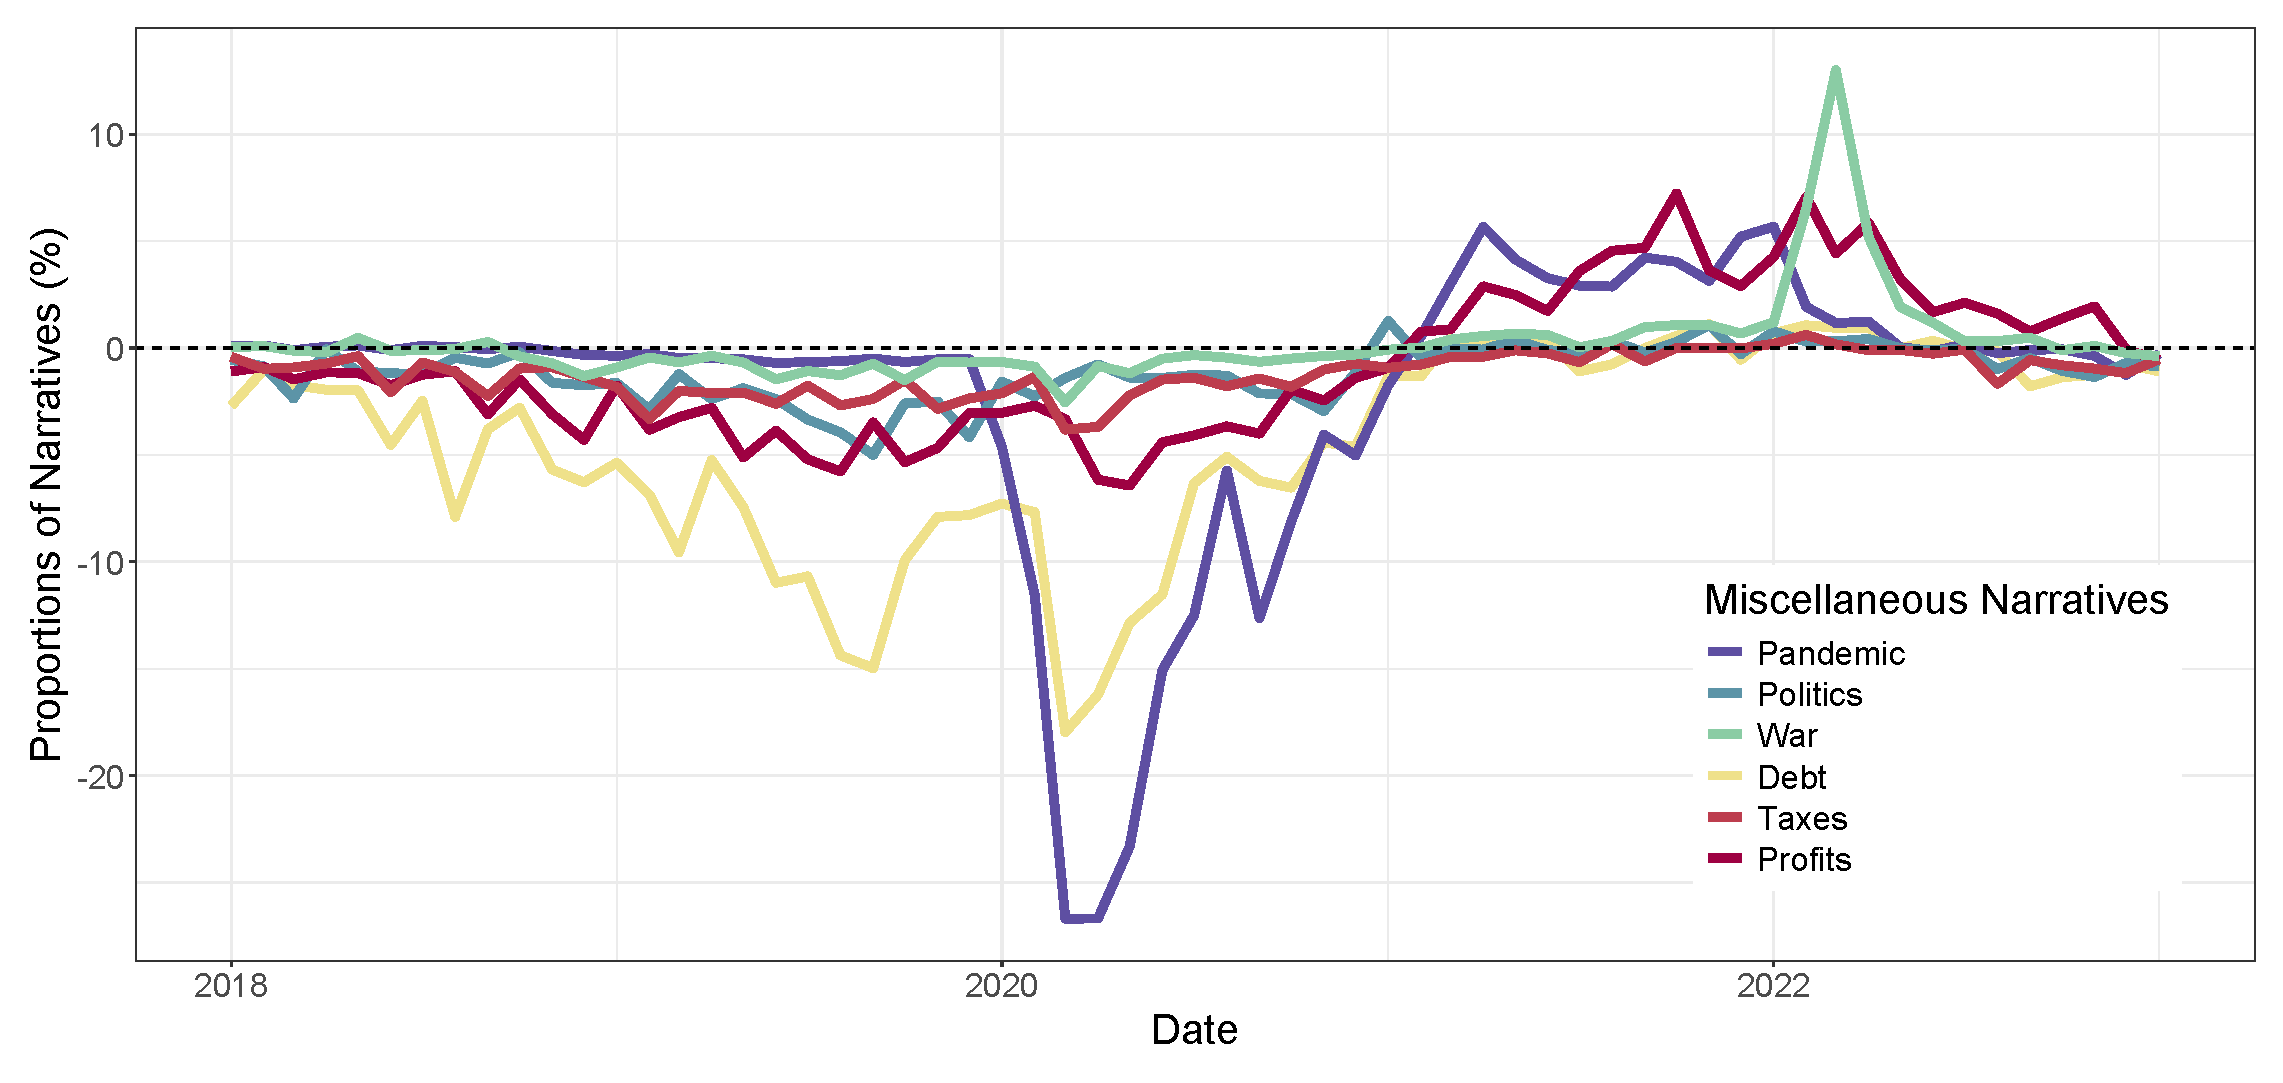
\includegraphics[width=\textwidth]{figures/plot_sothers.eps}
		\caption{Indices of miscellaneous narratives}
		\label{fig:sothers}
	\end{subfigure}
		\floatfoot{Note: The figures show the constructed narrative time series. Negative values signify the relative importance of a narrative in the context of falling inflation rates, whereas positive values represent the relative importance in the context of rising inflation rates.} 
\end{figure}

In contrast, the residual demand narrative reaches its minimum in early 2020, during the first announced economic lockdown following the COVID-19 outbreak. However, only a few months later, the narrative experiences significant positive growth. By 2021, it reaches relatively high positive values. The demand shift narrative also contributes to the media discourse about rising inflation rates but peaks with a lag compared to the demand (residual) narrative. Media reports on government spending as cause of inflation was not widespread during this entire period. We report only minor growth in late 2020 and early 2021. During this time, there were controversial discussions about large-scale infrastructure programs, which were questioned by Republicans and centrist Democrats (e.g., Peterson, 2021). In conclusion, we report positive values for all demand narratives from the beginning of 2021, but we observe significant differences in volume and timing.

Turning to the supply narratives, a similar trend becomes evident, with less negative values during the non-inflationary period. As Figure \ref{fig:ssupply} shows, only the energy narrative reaches profound negative values. In contrast, all four narratives show significant positive growth in 2020 and reach positive values in early 2021. Overall, all supply narratives follow a similar path, with the supply chain reporting the steepest increase, whereas the energy narrative is more volatile. Additionally, it is the first among supply narratives to experience negative values already in mid-2022. Only the labor shortage narrative reports a positive score until the end of the observation period.

Larger differences among the narratives do we report for the miscellaneous. As figure \ref{fig:sothers} shows, the tax and politics narratives experience only minor changes, however, there is a slight increase from the end of 2020 to early 2021 for the politics narrative. In contrast, the pandemic narrative records pronounced changes and is highly polarized. While non existing until end of 2019, it experienced a remarkable decline during early 2020. This is in line with the spread of the COVID-19 virus and the associated non-pharmaceutical measures. However, the pandemic narrative is also rapidly recovers, besides a smaller setback in late 2020. The debt narrative is primarily experiencing a profound negative score in 2020, while it remained more or less insignificant during the inflationary period. Characterized by fewer extremes, the profit narrative is present in both periods. Further, the narrative is more persistent during the inflationary period with a comparably late peak in 2022. Lastly, the war narrative is not existing until early 2022, which coincides with the invasion of Russia in the Ukraine. It rapidly declines afterwards.


\subsection{Granger Causality}

So far, our analysis has revealed two key findings. First, combining survey study results with a semi-supervised topic model and a latent sentiment scaling technique enables us to measure and quantify known concepts of inflation narratives. Thus we are able to describe their evolution over time and identify narrative-specific polarity. Second, we provide descriptive evidence on the spread of inflation narratives. For the considered time period, those emphasizing changes in demand and its
strong recovery, monetary policy, and supply issues as causes of inflation are particularly notable. Additionally, our descriptive analysis has shown that narratives on profits and specific crisis-related aspects, such as pandemic or war in Ukraine, are highly featured in news media articles. In contrast, other narratives, including those on government spending, politics, debt, and taxes, are less often featured in reports about rising inflation rates.
	
To deepen our understanding of how inflation narratives interact with the macroeconomy, especially inflation expectations, we first construct multiple multivariate VAR models to test for potential Granger causalities in our system. The VAR models include short-term and mid-term expectations, CPI inflation, economic activity and one of the measured narrative indices. Even tough the procedure is based on predictability, and not on direct causal effects, we follow Granger's argument that predictive power can serve as an indicator for potential causalities \citep{shojaie.2022}. Additionally, by applying the test procedure in a more restrictive VAR setting we control relevant information beyond a bivariate relationship. In a second step we take existing economic research into account that indicates strong variations of inflation expectations among different socioeconomic groups (e.g., \citet{ecb.2021, Weber.etal.2022}). Further, pioneer survey studies suggest that the narratives of households are diverse and systematically related to individual characteristics (e.g., \citet{Andre.2023, Demgensky.2023}). To address this variation, we analyze disaggregated household expectations based on income, education, age, and numeracy, employing data from the New York Fed Survey of Consumer Expectations. Afterwards, we re-estimate our multivariate Granger causality tests by incorporating the expectations of subgroups (e.g. low income or high educated households) from each socioeconomic category to identify any potential Granger causal relationships.

\subsubsection{Aggregated Expectations}

As discussed in Chapter \ref{sec:MethodsData}, we treat all variables as trend-cycle filtered series and use them as baseline estimates. For robustness, we provide level and difference estimations in the Online Appendix. The results of the baseline estimation are shown in table \ref{tab:granger_bHP}. It provides a comprehensive overview of all p-values of the Granger causality analysis, indicating whether or not a narrative is Granger-causing 1-year or 3-year expectations. Thus, we test whether the integration of a narrative lag into a system of lagged variables improves the prediction of the households' expectations. As the table shows, we report several significant Granger-causal relationships.

For the demand narratives, we report significant results exclusively for the government spending narrative at the aggregate level (medium-term). For short-term expectations, we identify Granger-causal relationships for the supply chain and labor shortage narratives. For medium-term expectations, thee relationships for the supply chain narrative persists, though only at the 10-percent level. Further Granger causality relationships are observed for miscellaneous narratives, including the war and profits narratives, for both short-term and medium-term expectations. In addition, we examine potential feedback relationships in table \ref{tab:granger_bHP_feedback}. We test the exogeneity of the narratives with respect to aggregate expectations. Among the previous Granger causalities, our estimation suggests a feedback relationship with 3-year expectations only for the energy and labor shortage narrative. We also find some reverse Granger causality for the demand (residual), energy, and supply (residual) narratives from 1-year expectations.

\begin{table}[ht]
\centering
\caption{Narrative $\rightarrow$ Expectations Granger causality (boosted HP-Filter)}\label{tab:granger_bHP}

\begin{tabular}{lcc}
\toprule
\textbf{Narratives} & \textbf{One-Year Expectations} & \textbf{Three-Year Expectations} \\
& (Pr($>$F)) & (Pr($>$F)) \\
\midrule
\multicolumn{3}{l}{\textbf{Demand}} \\
\midrule
Government Spending & 0.29 & 0.09 * \\
Monetary Policy & 0.64 & 0.23 \\
Demand Shift & 0.16 & 0.41 \\
Demand (residual) & 0.80 & 0.96 \\
\midrule
\multicolumn{3}{l}{\textbf{Supply}} \\
\midrule
Supply Chain & $<$0.01 *** & 0.10 * \\
Energy & 0.75 & 0.34 \\
Labor Shortage & $<$0.01 *** & 0.38 \\
Supply (residual) & 0.52 & 0.39 \\
\midrule
\multicolumn{3}{l}{\textbf{Miscellaneous}} \\
\midrule
Pandemic & 0.39 & 0.23 \\
Politics & 0.57 & 0.95 \\
War & 0.04 ** & 0.04 ** \\
Debt & 0.11 & 0.86 \\
Taxes & 0.91 & 0.29 \\
Profits & 0.02 ** & $<$0.01 *** \\
\midrule
\bottomrule
\textit{Note:}  & \multicolumn{2}{r}{$^{*}$p$<$0.1; $^{**}$p$<$0.05; $^{***}$p$<$0.01} \\
\bottomrule
\end{tabular}
\end{table}


To ensure robustness, we provide additional level and difference estimations in the Online Appendix in Tables \ref{tab:granger_level} and \ref{tab:granger_diff}. Overall, the results for the supply chain and profits narratives using the boosted HP filter are confirmed by both robustness checks. Additionally, the difference estimation supports the findings for the government spending narrative, while the level does not. In contrast, the level estimates reveal more significant relationships. Unlike the trend-cycle filtered estimation, the level estimates indicate additional Granger causality for monetary policy, demand shift, supply residuals, debt, and politics on 3-year expectations. For the demand shift narrative, significant findings are observed for both short-term and medium-term expectations. In contrast, the differenced time series analysis reveals additional significant results only for the demand shift for short-term expectations.

At last,  our results suggest that narratives featured in media reports possess inherent statistical predictive power for household expectations. This can be interpreted as an indicator of potential causalities \cite{shojaie.2022}. Moreover, our findings suggest that Granger causalities are present in all categories, but there are slight differences in the data between short-term and medium-term expectations.  To address the challenge of potential nonstationarity, we consider results with three different estimation strategies. Although we find some differences between these estimations, most of the results, especially for short-term expectations, are confirmed. Moreover, correlative evidence from \cite{Andre.2023} and \cite{Stantcheva.2024} backs our findings regarding how important supply and profit narratives are for 1-year expectations. In contrast to these survey studies, we do not report significant p-values for the politics, monetary policy, and government spending narratives on aggregate expectations. This could be partly explained by the considered news source, which targets financial market actors and experts. 

\begin{table}[ht]
\centering
\footnotesize
\caption{Expectations $\rightarrow$ Narrative Granger causality (boosted HP-Filter)}\label{tab:granger_bHP_feedback}

\begin{tabular}{lcccc}
\toprule
\textbf{Narratives} & \textbf{One-Year Expectations} & \textbf{Three-Year Expectations} & \textbf{CPI Inflation} & \textbf{Economic Activity} \\
& (Pr($>$F)) & (Pr($>$F)) & (Pr($>$F)) & (Pr($>$F)) \\
\midrule
\multicolumn{5}{l}{\textbf{Demand}} \\
\midrule
Government Spending & 0.563 & 0.854&0.766&0.964 \\
Monetary Policy & 0.644 & 0.539&0.414&0.766 \\
Demand Shift & 0.778 & 0.585&0.076 *&0.616 \\
Demand (residual) & $<$0.01 *** & 0.322&0.010 **&0.405 \\
\midrule
\multicolumn{5}{l}{\textbf{Supply}} \\
\midrule
Supply Chain & 0.162 & 0.198&0.965&0.410 \\
Energy & 0.054 * & 0.022 **&0.669&0.873 \\
Labor Shortage & 0.422 & 0.036 **&0.314&0.957 \\
Supply (residual) & 0.039 ** & 0.531&0.010 **&0.674 \\
\midrule
\multicolumn{5}{l}{\textbf{Miscellaneous}} \\
\midrule
Pandemic & 0.121 & 0.299&0.198&0.704 \\
Politics & 0.895 & 0.971&0.261&0.692 \\
War & 0.930 & 0.751&0.900&0.948 \\
Debt & 0.406 & 0.891&0.394&0.995 \\
Taxes & 0.495 & 0.883&0.075 *&0.295 \\
Profits & 0.730 & 0.731&0.255&0.417 \\
\midrule
\bottomrule
\textit{Note:}  & \multicolumn{4}{r}{$^{*}$p$<$0.1; $^{**}$p$<$0.05; $^{***}$p$<$0.01} \\
\bottomrule
\end{tabular}
\end{table}


\subsubsection{Socioeconomic Heterogeneity}

\textbf{Heterogeneity by Income} - We begin the discussion of socioeconomic heterogeneity by looking at differences in income. The New York Fed survey distinguishes three income groups: below \$50k, \$50k to \$100k, and above \$100k per year. The results in table \ref{tab:granger_bHP_income} in the Online Appendix show some differences between the considered groups. With respect to short-term expectations, our results suggest only small distinctions between the different income groups. The supply chain, labor shortage, war, and profit narratives are significant for all income groups. However, variations in the supply (residual) and demand shift narratives are observed: these are significant for low- and high-income households but not for middle-income households. In contrast, greater differences across income groups emerge for medium-term expectations. Our results highlight the importance of demand narratives for middle- and high-income households, while lower-income households show significant effects only for the energy and profits narratives. For 3-year expectations, middle-income households respond predominantly to demand narratives, with the exception of the supply (residual) narrative. In contrast, high-income households exhibit multiple Granger causal relationships, encompassing demand, supply, and miscellaneous narratives.\\


\noindent \textbf{Heterogeneity by Education} - To access further potential heterogeneity of narratives across socioeconomic groups, we conduct Granger tests for different educational backgrounds of households. Accordingly, we consider the household groups with a high school degree or less, some college, and a BA or higher. The results are shown in table \ref{tab:granger_bHP_educ} in the Online Appendix. The findings highlight the overall importance of the government spending, supply chain, war, and profits narratives, as reflected in the aggregated expectations analysis.  However, households with high levels of education appear more responsive to narratives emphasizing demand shifts, supply chain issues and energy prices (both for medium-term expectations). While we observe a Granger causality from the war narrative to short-term expectations for households with some college degree or less, we do not confirm this for households with a BA or higher. Notably, a Granger causality for medium-term expectations of households with a high school degree or less is identified exclusively for the government spending narrative.\\

\noindent \textbf{Heterogeneity by Age} - Pronounced variations with respect to age are visible in \ref{tab:granger_bHP_age} in the Online Appendix. As before, we observe less heterogeneity across different ages for medium-term expectations than for short-term expectations. For the analysis, we consider three age groups: under 40, 40 to 59, and over 59. In general, demand narratives are more relevant for households aged 40 and older. Additionally, several supply narratives significantly influence short-term expectations for these households. In contrast, the youngest cohort shows the strongest Granger-causal relationships with miscellaneous narratives. In summary, this analysis supports the aggregated results while emphasizing the importance of age as a determinant of heterogeneity across households. \\

\noindent\textbf{Heterogeneity by Numeracy} - Finally, we examine potential heterogeneity between households with low and high numeracy in table \ref{tab:granger_bHP_num} in the Online Appendix. Overall, our analysis indicates no substantial differences between the two groups of households based on numeracy, aside from minor variations in the significance level of specific narratives. For Households with lower numeracy our analysis shows smaller significance levels for the war narrative, while for those with higher numeracy we observe smaller significance levels especially for the supply chain and labor shortage narratives.

\subsubsection{Dynamic Responses}

To further investigate potential causal relationships between our narratives and households' expectations, we estimate impulse responses. This approach allows us to gain a more comprehensive understanding of the impact that an increasing diffusion of narratives has at the macroeconomic level. In the following section, we provide an overview of the impulse responses that we conducted by means of \cite{Jorda.2005}'s local projections. In this process, the impulse responses measure the effect of an impulse to the system, i.e. how an impulse at a specific point of time $t_0$ in one equation proceeds through a system \citep[138]{Kirchgaesser.2007}. In this case, we consider a shock the size of one standard deviation of the error term. We conduct several multivariate models that contain five different variables: 1-year and 3-year expected inflation by households, CPI inflation, economic activity, and one of our constructed narrative indices. Again, as mentioned in chapter \ref{subsec:methods}, we treat all variables as trend-cycle filtered time series and use them as a baseline. For the robustness, we estimated the local projections with levels and differences. To ensure readability and an efficient use of the limited space, we included all graphical illustrations of the impulse responses in the Online Appendix. The complete set of baseline impulse responses are illustrated in figure \ref{fig:irf_1}, \ref{fig:irf_2}, \ref{fig:irf_3}, and \ref{fig:irf_4} in the Online Appendix. Figure \ref{fig:irf_base} reports a selection of significant responses. The x-axis represents the forecast horizon $s$, with a maximum of 12 months, while the y-axis shows the change in 1- or 3-year household expectations in response to a standardized deviation innovation. The black line represents the mean response to a shock, while the gray area around the line visualizes the 90\% confidence interval.

We begin by examining the response to demand narrative shocks. In doing so, we observe statistically significant positive responses for all demand narratives. Comparatively, we note some differences in the paths and the magnitude of these responses. The shock in the government spending narrative is the longest lasting and with the largest magnitude. The response in the monetary policy narrative follows a similar path but on lower levels, while a shock in the demand shift narrative is only in initially significantly positive. Medium-term expectations react to a shock in the demand (residual) narrative after 6 months, but are largely not significant. These findings are consistent with the positive coefficients for the monetary policy and government spending narratives in \cite{Andre.2023}. The impulse responses for the supply chain narrative are in line with the discussion about its anchoring tendency in \cite{Andre.2023} and \cite{Demgensky.2023}. The response is short-lived and temporarily negative. While there is a primarily statistically insignificant reaction for the energy and supply (residual) narrative, the relevance of the supply chain and labor shortage narrative for household expectations is again highlighted. For the latter, the response is more profound, but also only lasting for up to 6 months. Finally, the ways in which the miscellaneous narratives react to a shock are more diverse, with a large number of responses being insignificant. We establish significant results for short-term expectations to a shock in the pandemic narrative, which are initially negative, before they turn positive over time. In contrast, a shock to the politics narrative seems to initially raise expectations, especially in the medium-term, and then return to the baseline. We do not report any significant responses to a shock in the debt or taxes narrative. Furthermore, the war narrative and the profits narrative should be emphasized. The profits narrative indicates positive responses in both expectations, which are also relatively strong in terms of magnitude, with a rather transient effect on 3-year expectations. The response to the war narrative is exceptional considering its strong decreasing tendency after an initial increase, following a reversed course to a shock in the pandemic narrative. Overall, the results are roughly in line with our previous findings and the results of the survey conducted by \cite{Andre.2023, Stantcheva.2024, Demgensky.2023}. 


\begin{figure}[H]
	\centering
	\captionsetup{font=footnotesize}
	\begin{subfigure}{00.32\textwidth}
		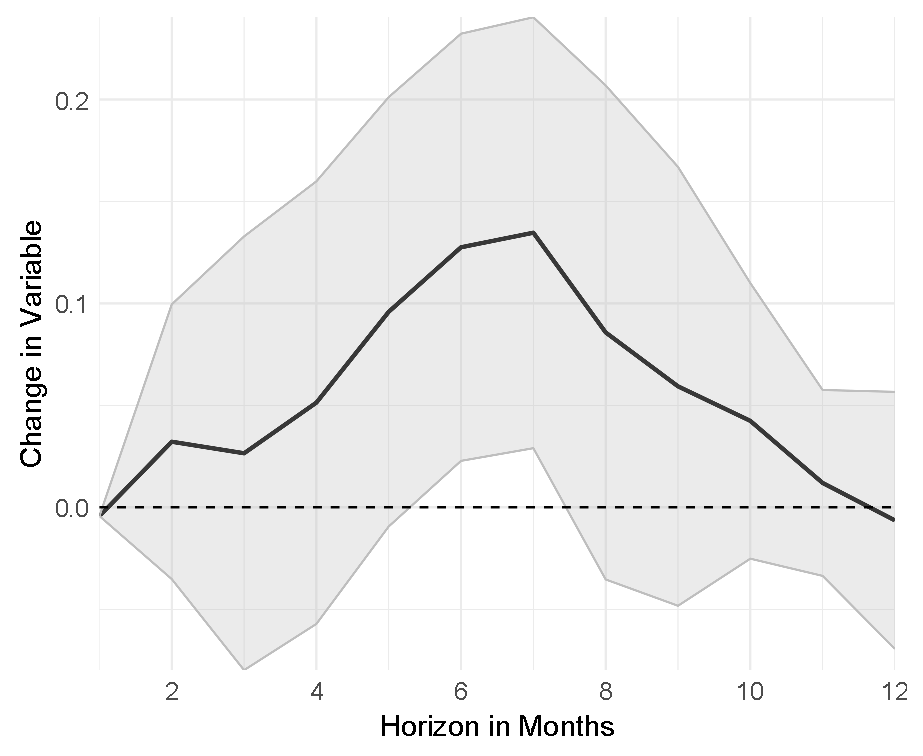
\includegraphics[width=1\textwidth]{output/lp/baseline/bHP/government_spending/government_spendingonexpectations1y_djn.eps}
		\caption{Government spending on 1-year}
	\end{subfigure}
	\begin{subfigure}{00.32\textwidth}
		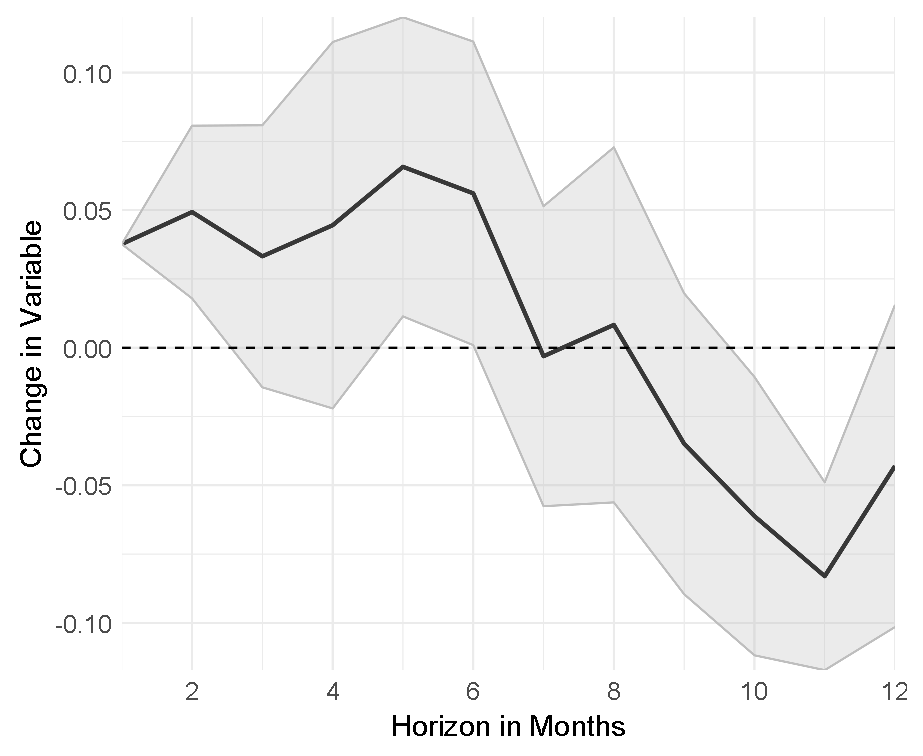
\includegraphics[width=1\textwidth]{output/lp/baseline/bHP/monetary_policy/monetary_policyonexpectations1y_djn.eps}
		\caption{Monetary policy on 1-year}
	\end{subfigure}
	\begin{subfigure}{00.32\textwidth}
		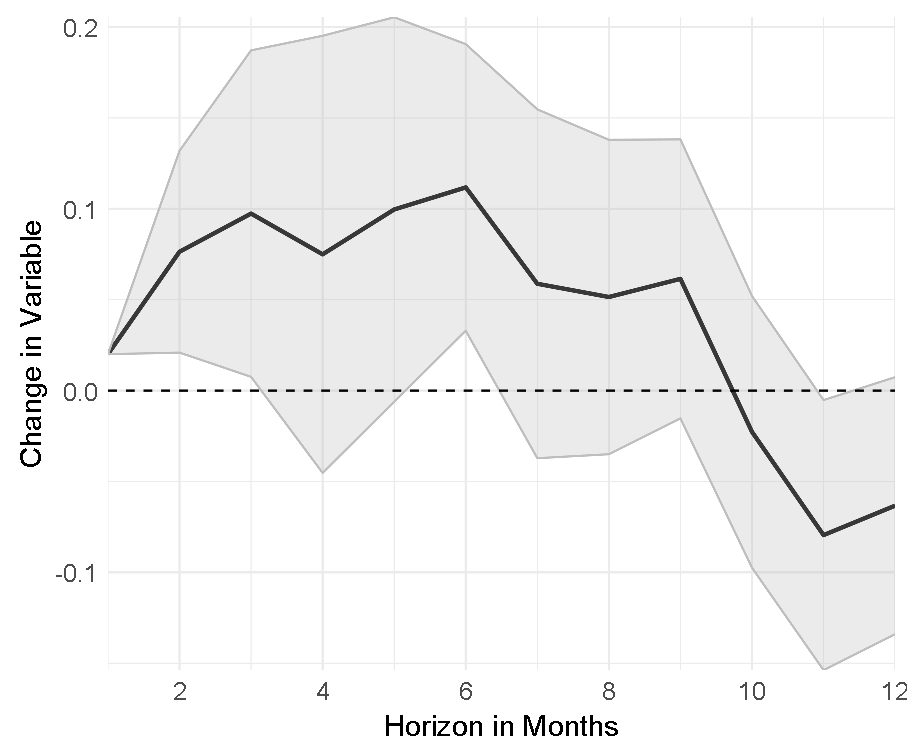
\includegraphics[width=1\textwidth]{output/lp/baseline/bHP/supply_chain/supply_chainonexpectations1y_djn.eps}
		\caption{Supply chain on 1-year}
	\end{subfigure}
	\begin{subfigure}{00.32\textwidth}
		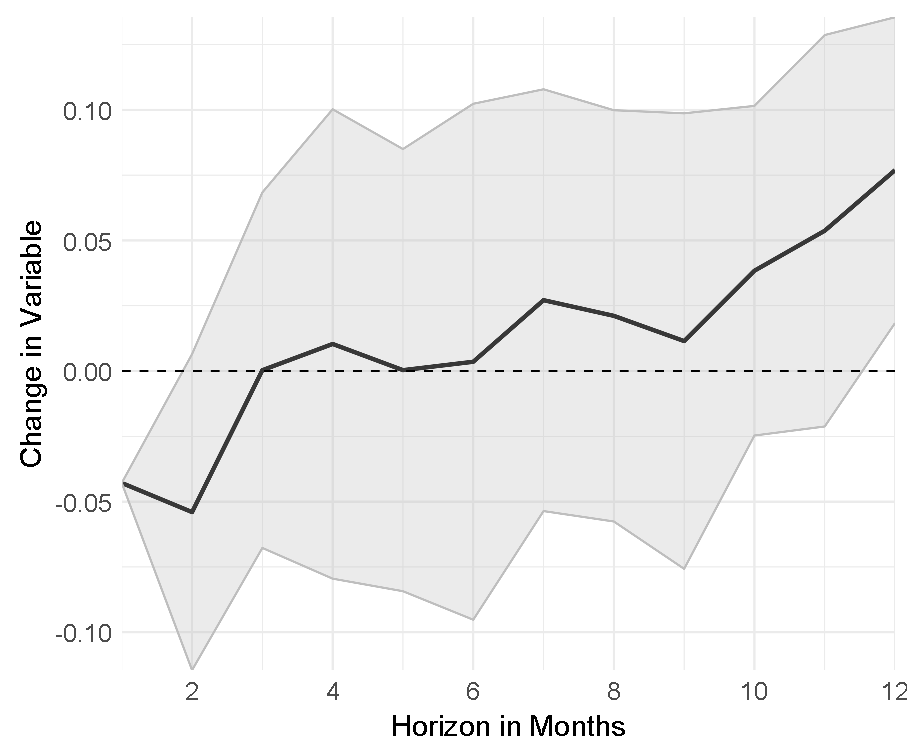
\includegraphics[width=1\textwidth]{output/lp/baseline/bHP/pandemic/pandemiconexpectations1y_djn.eps}
		\caption{Pandemic on 1-year}
	\end{subfigure}
	\begin{subfigure}{00.32\textwidth}
		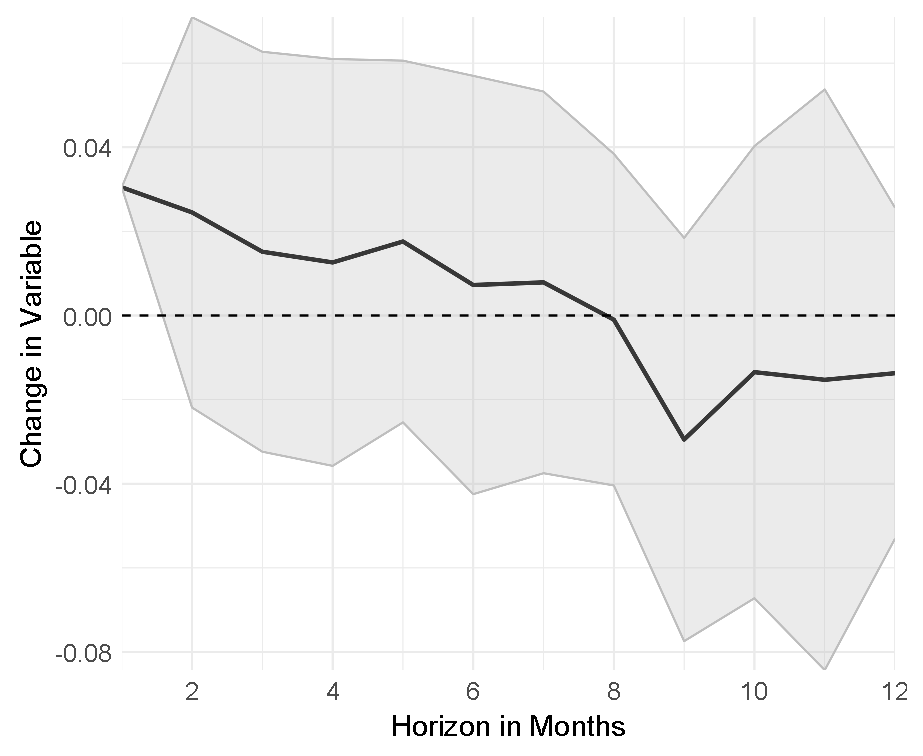
\includegraphics[width=1\textwidth]{output/lp/baseline/bHP/politics/politicsonexpectations3y_djn.eps}
		\caption{Politics on 3-year}
	\end{subfigure}
	\begin{subfigure}{00.32\textwidth}
		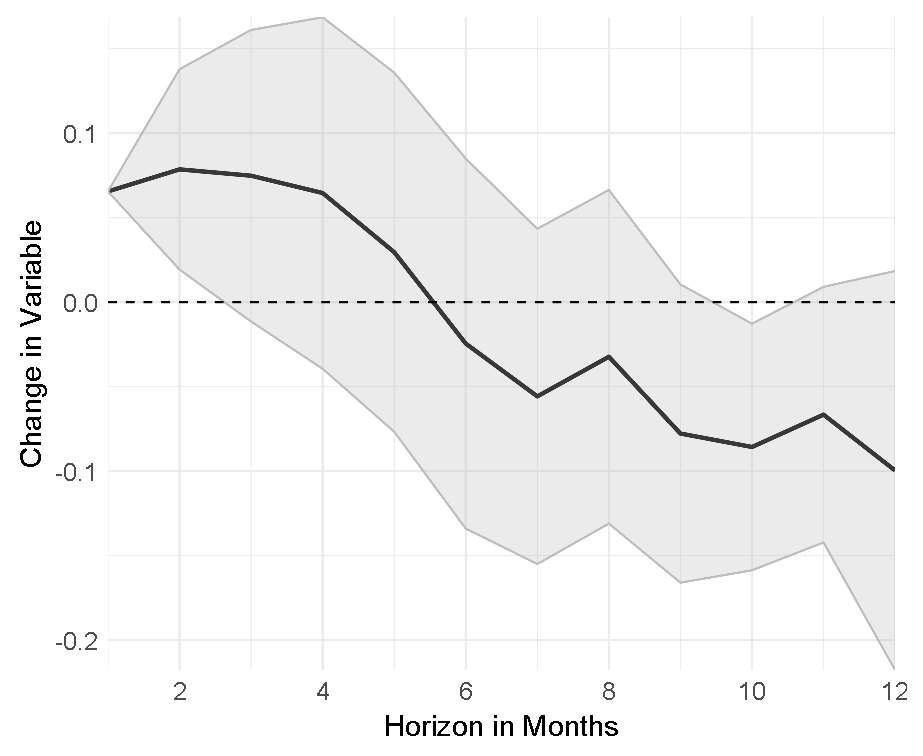
\includegraphics[width=1\textwidth]{output/lp/baseline/bHP/war/waronexpectations1y_djn.eps}
		\caption{War on 1-year}
	\end{subfigure}
	\begin{subfigure}{00.32\textwidth}
		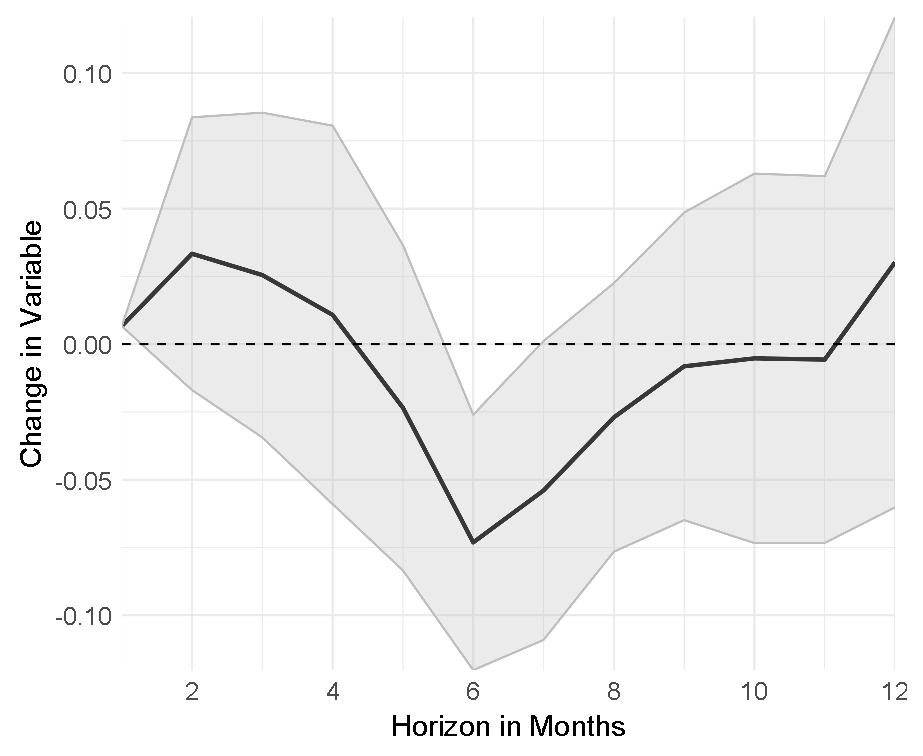
\includegraphics[width=1\textwidth]{output/lp/baseline/bHP/war/waronexpectations3y_djn.eps}
		\caption{War on 3-year}
	\end{subfigure}
	\begin{subfigure}{00.32\textwidth}
		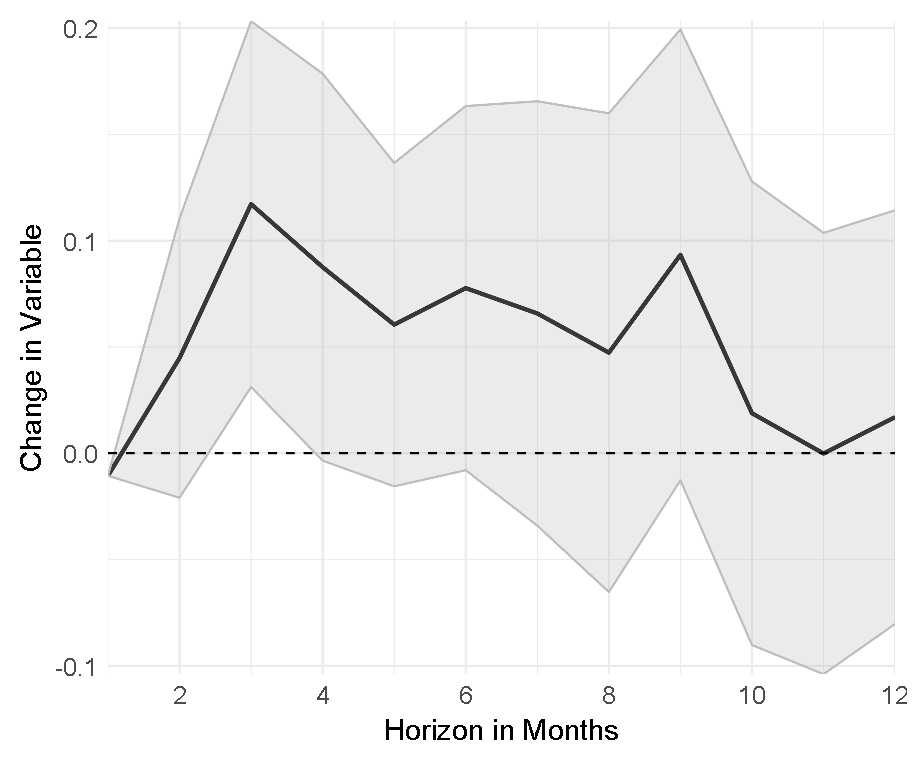
\includegraphics[width=1\textwidth]{output/lp/baseline/bHP/profits/profitsonexpectations1y_djn.eps}
		\caption{Profits on 1-year}
	\end{subfigure}
	\begin{subfigure}{00.32\textwidth}
		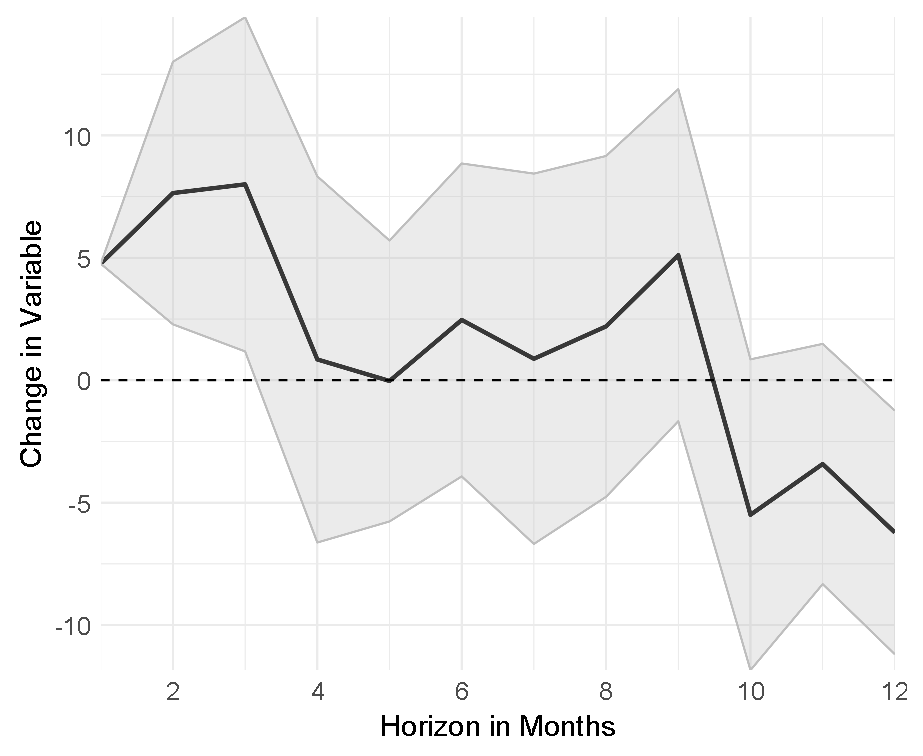
\includegraphics[width=1\textwidth]{output/lp/baseline/bHP/profits/profitsonexpectations3y_djn.eps}
		\caption{Profits on 3-year}
	\end{subfigure}
	\caption{Selection of narratives' impulse responses}
	\label{fig:irf_base}
	\floatfoot{Note: The graphs show the mean responses and 90\% confidence bands. The x-axis shows months (s) after narrative diffusion event; t = 0 is the month of the shock event. The y-axis shows the change in expectations as a response to the shock event. The shock considered is of the size of one standard deviation.}
\end{figure}


To summarize the analysis of aggregate expectations, it can be concluded that a (positive) narrative shock is followed by an initial positive response of households' expectations. At the same time, a closer look reveals differences in the paths of the responses. Comparing 1-year and 3-year expectations, the response in 1-year expectations is more pronounced in terms of magnitude and, in many cases, more persistent. The results also highlight some important differences between the narratives. While our results indicate significant positive responses for most demand and supply narratives, the responses of the latter are less persistent and in some cases across large parts insignificant for 3-year expectations, suggesting a stronger anchoring tendency of these narratives. On the other hand, the responses to a shock in the miscellaneous narratives are more diverse. Among these, the profits, war, and pandemic narrative stands out for their effects on short-term expectations.

As for the Granger causality tests, we provide robustness estimates again using levels and differences. The results for the selected impulse responses from figure \ref{fig:irf_base} are shown in the Online Appendix with level specification in figure \ref{fig:irf_level}, and figure \ref{fig:irf_diff} visualized the results with the differences. While the responses under level specification are more persistent, the responses with differences time series are more ambivalent and unstable. In general, the robustness estimations support our findings. However, for the pandemic narrative only, both robustness estimations indicate no significant reaction in household expectations. It should be noted, that the baseline estimation indicates an overall stronger anchoring tendency of expectations.


% Here: Conclusion
% !TeX spellcheck = en_US
\section{Conclusion}\label{sec:Conclusion}


This paper proposes a new methodological approach to measure known inflation narratives in news reports. The combination of survey information on inflation narratives with a supervised topic model and a latent semantic scaling approach provides information on the prevalence and spread of narratives in a large text corpus, including the Wall Street Journal. For the recent inflationary period, our descriptive results highlight the presence of narratives about changing demand, supply factors including the supply chain, energy prices, and labor shortages, as well as stories about the war in Ukraine and corporate profits. Conversely, narratives about monetary policy, government debt, and the pandemic were prevalent in the preceding period of low inflation and deflation, respectively. To further investigate the relevance for macroeconomic development, additional time series analyses were conducted. As suggested by the multivariate Granger causality tests, the considered narratives contain relevant information for households' expectations. This is in line with the theoretical arguments presented in \cite{Shiller.2017, Tuckett.2020} and \cite{Beckert.2016}. While our estimates suggest only small differences between short- and medium-term aggregate expectations, we highlight heterogeneity across socioeconomic groups. We document notable differences in income, education, and age, especially for medium-term expectations. For example, our results imply that the energy and corporate profits narrative is the main driver of 3-year expectations for households with lower annual incomes, while several narratives Granger-cause the expectations of high-income households. In addition, our analysis points to the importance of age as a driver of heterogeneity. To further investigate potential differences in the pathways of responses to narrative diffusion, we conduct impulse responses. Our estimates show that the responses to 1-year expectations are more pronounced and often more persistent. Moreover, when comparing shocks across narratives, we notice more anchored expectations with respect to a shock in the supply chain, demand shift, and profits narratives.

In summary, our paper reveals the powerful role  that media narratives play in shaping economic expectations, potentially anchoring or unanchoring inflation expectations over time. This impact varies by narrative type and socioeconomic backgrounds of households, making it  particularly relevant for monetary policymakers, who may pay even more attention to media coverage. By recognizing the diverse impact of these narratives, policymakers can develop more targeted communication strategies. Future advances in narrative analysis hold the promise of enabling even more responsive and adaptable policy interventions, aligned with the evolving narratives captured in media.

% References
\newpage
%\footnotesize
	\bibliographystyle{aer}
	\bibliography{./bibtex/literaturverzeichnis_inflation.bib,./bibtex/Masterarbeit.bib,./bibtex/biblio.bib,./bibtex/pub_uf.bib}
\normalsize


% Here: Appendix (new page)
%\newpage
% !TeX spellcheck = en_US
% Appendices
\clearpage
\appendix
\pagenumbering{Roman}  % Change page numbering to Roman numerals
\setcounter{page}{1}   % Start numbering from I
\newpage
\counterwithin{figure}{section} % Setzt den Figure-Zähler auf Abschnitt-Ebene zurück
\counterwithin{table}{section} % Setzt den Figure-Zähler auf Abschnitt-Ebene zurück
\section{Appendix - Going Viral: Inflation Narratives and the Macroeconomy}\label{sec:Appendix}

\subsection{Supplementary Figures and Tables}\label{subsec:Supplements}

\begin{figure}[h]
	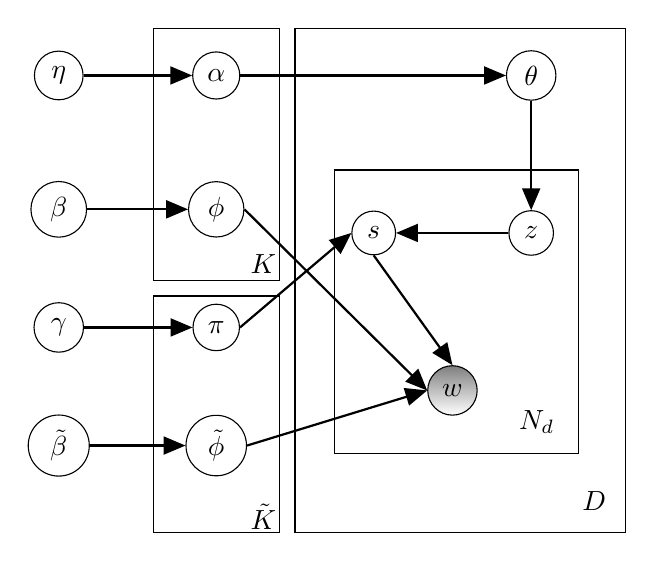
\begin{tikzpicture}
		%\node (p) at (-4,2) [circle,draw] {$\bm{P}$};
		%\node (htd) at (0,2) [circle,draw] {$h_{t[d]}$};
		\node (theta) at (0,0) [circle, draw] {$\theta$};
		\node (z) at (0,-2) [circle, draw] {$z$};
		\node (s) at (-2,-2) [circle, draw] {$s$};
		\node (a) at (-4,0) [circle, draw] {$\alpha$};
		\node (phi) at (-4,-1.7) [circle,draw] {$\phi$};
		\node (w) at (-1,-4) [shade,circle,draw] {$w$};
		\node (eta) at (-6,0) [circle,draw] {$\eta$};
		\node (beta) at (-6,-1.7) [circle,draw] {$\beta$};
		
		\node (gamma) at (-6,-3.2) [circle,draw] {$\gamma$};
		\node (pi) at (-4,-3.2) [circle,draw] {$\pi$};
		
		\node (tbeta) at (-6,-4.7) [circle,draw] {$\tilde{\beta}$};
		\node (tphi) at (-4,-4.7) [circle,draw] {$\tilde{\phi}$};
		
		
		%\draw[thick,->] (p.east) -- (htd.west);
		\draw[thick,->] (a.east) -- (theta.west);
		\draw[thick,->] (phi.east) -- (w.west);
		\draw[thick,->] (z.west) -- (s.east);
		\draw[thick,->] (s.south) -- (w.north);
		\draw[thick,->] (eta.east) -- (a.west);
		\draw[thick,->] (beta.east) -- (phi.west);
		%&\draw[thick,->] (htd.south) -- (theta.north);
		\draw[thick,->] (theta.south) -- (z.north);
		
		\draw[thick,->] (gamma.east) -- (pi.west);
		\draw[thick,->] (tbeta.east) -- (tphi.west);
		
		\draw[thick,->] (pi.east) -- (s.west);
		\draw[thick,->] (tphi.east) -- (w.west);
		
		\draw (-3,-5.8) rectangle (1.2,.6);
		\draw (-2.5,-4.8) rectangle (0.6,-1.2);
		\draw (-4.8,-2.6) rectangle (-3.2,.6);
		
		%\draw (-4.8,-2.6) rectangle (-3.2,-1.2);
		\draw (-4.8,-5.8) rectangle (-3.2,-2.8);
		
		\node at (0.07,-4.4) {$N_d$};
		
		\node at (0.8,-5.4) {$D$};
		
		%\node at (-3.4,-0.6) {$R$};
		\node at (-3.4,-2.4) {$K$};	
		\node at (-3.4,-5.6) {$\tilde{K}$};
		
		
		
	\end{tikzpicture}
	\caption{Graphical model of base keyATM}
	\label{graph:basekeyatm}
	\floatfoot{The shaded node ($w$) denotes observed variables, while other transparent nodes denote latent variables. Source: \cite[40]{Eshima.2020}}
\end{figure}

\begin{figure}[H]
	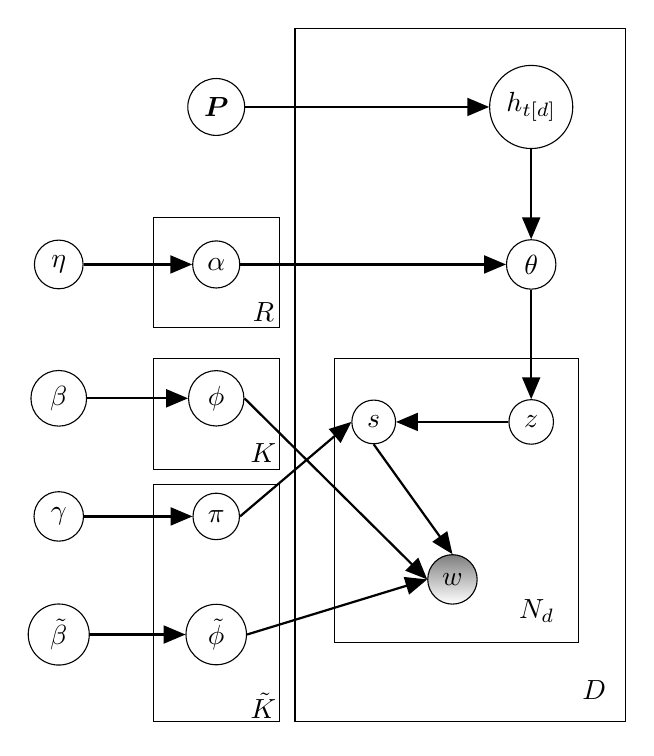
\begin{tikzpicture}
		\node (p) at (-4,2) [circle,draw] {$\bm{P}$};
		\node (htd) at (0,2) [circle,draw] {$h_{t[d]}$};
		\node (theta) at (0,0) [circle, draw] {$\theta$};
		\node (z) at (0,-2) [circle, draw] {$z$};
		\node (s) at (-2,-2) [circle, draw] {$s$};
		\node (a) at (-4,0) [circle, draw] {$\alpha$};
		\node (phi) at (-4,-1.7) [circle,draw] {$\phi$};
		\node (w) at (-1,-4) [shade,circle,draw] {$w$};
		\node (eta) at (-6,0) [circle,draw] {$\eta$};
		\node (beta) at (-6,-1.7) [circle,draw] {$\beta$};
		
		\node (gamma) at (-6,-3.2) [circle,draw] {$\gamma$};
		\node (pi) at (-4,-3.2) [circle,draw] {$\pi$};
		
		\node (tbeta) at (-6,-4.7) [circle,draw] {$\tilde{\beta}$};
		\node (tphi) at (-4,-4.7) [circle,draw] {$\tilde{\phi}$};
		
		
		\draw[thick,->] (p.east) -- (htd.west);
		\draw[thick,->] (a.east) -- (theta.west);
		\draw[thick,->] (phi.east) -- (w.west);
		\draw[thick,->] (z.west) -- (s.east);
		\draw[thick,->] (s.south) -- (w.north);
		\draw[thick,->] (eta.east) -- (a.west);
		\draw[thick,->] (beta.east) -- (phi.west);
		\draw[thick,->] (htd.south) -- (theta.north);
		\draw[thick,->] (theta.south) -- (z.north);
		
		\draw[thick,->] (gamma.east) -- (pi.west);
		\draw[thick,->] (tbeta.east) -- (tphi.west);
		
		\draw[thick,->] (pi.east) -- (s.west);
		\draw[thick,->] (tphi.east) -- (w.west);
		
		\draw (-3,-5.8) rectangle (1.2,3);
		\draw (-2.5,-4.8) rectangle (0.6,-1.2);
		\draw (-4.8,-0.8) rectangle (-3.2,0.6);
		
		\draw (-4.8,-2.6) rectangle (-3.2,-1.2);
		\draw (-4.8,-5.8) rectangle (-3.2,-2.8);
		
		\node at (0.07,-4.4) {$N_d$};
		
		\node at (0.8,-5.4) {$D$};
		
		\node at (-3.4,-0.6) {$R$};
		\node at (-3.4,-2.4) {$K$};	
		\node at (-3.4,-5.6) {$\tilde{K}$};
		
	\end{tikzpicture}
	\caption{Graphical model of dynamic \textsf{\textbf{keyATM}}}
	\label{graph:dynamickeyatm}
	\floatfoot{The shaded node ($w$) denotes observed variables, while other transparent nodes denote latent variables. Source: \cite[41]{Eshima.2020}}
\end{figure}	


%Modelfit Graphic
\begin{figure}[H]
	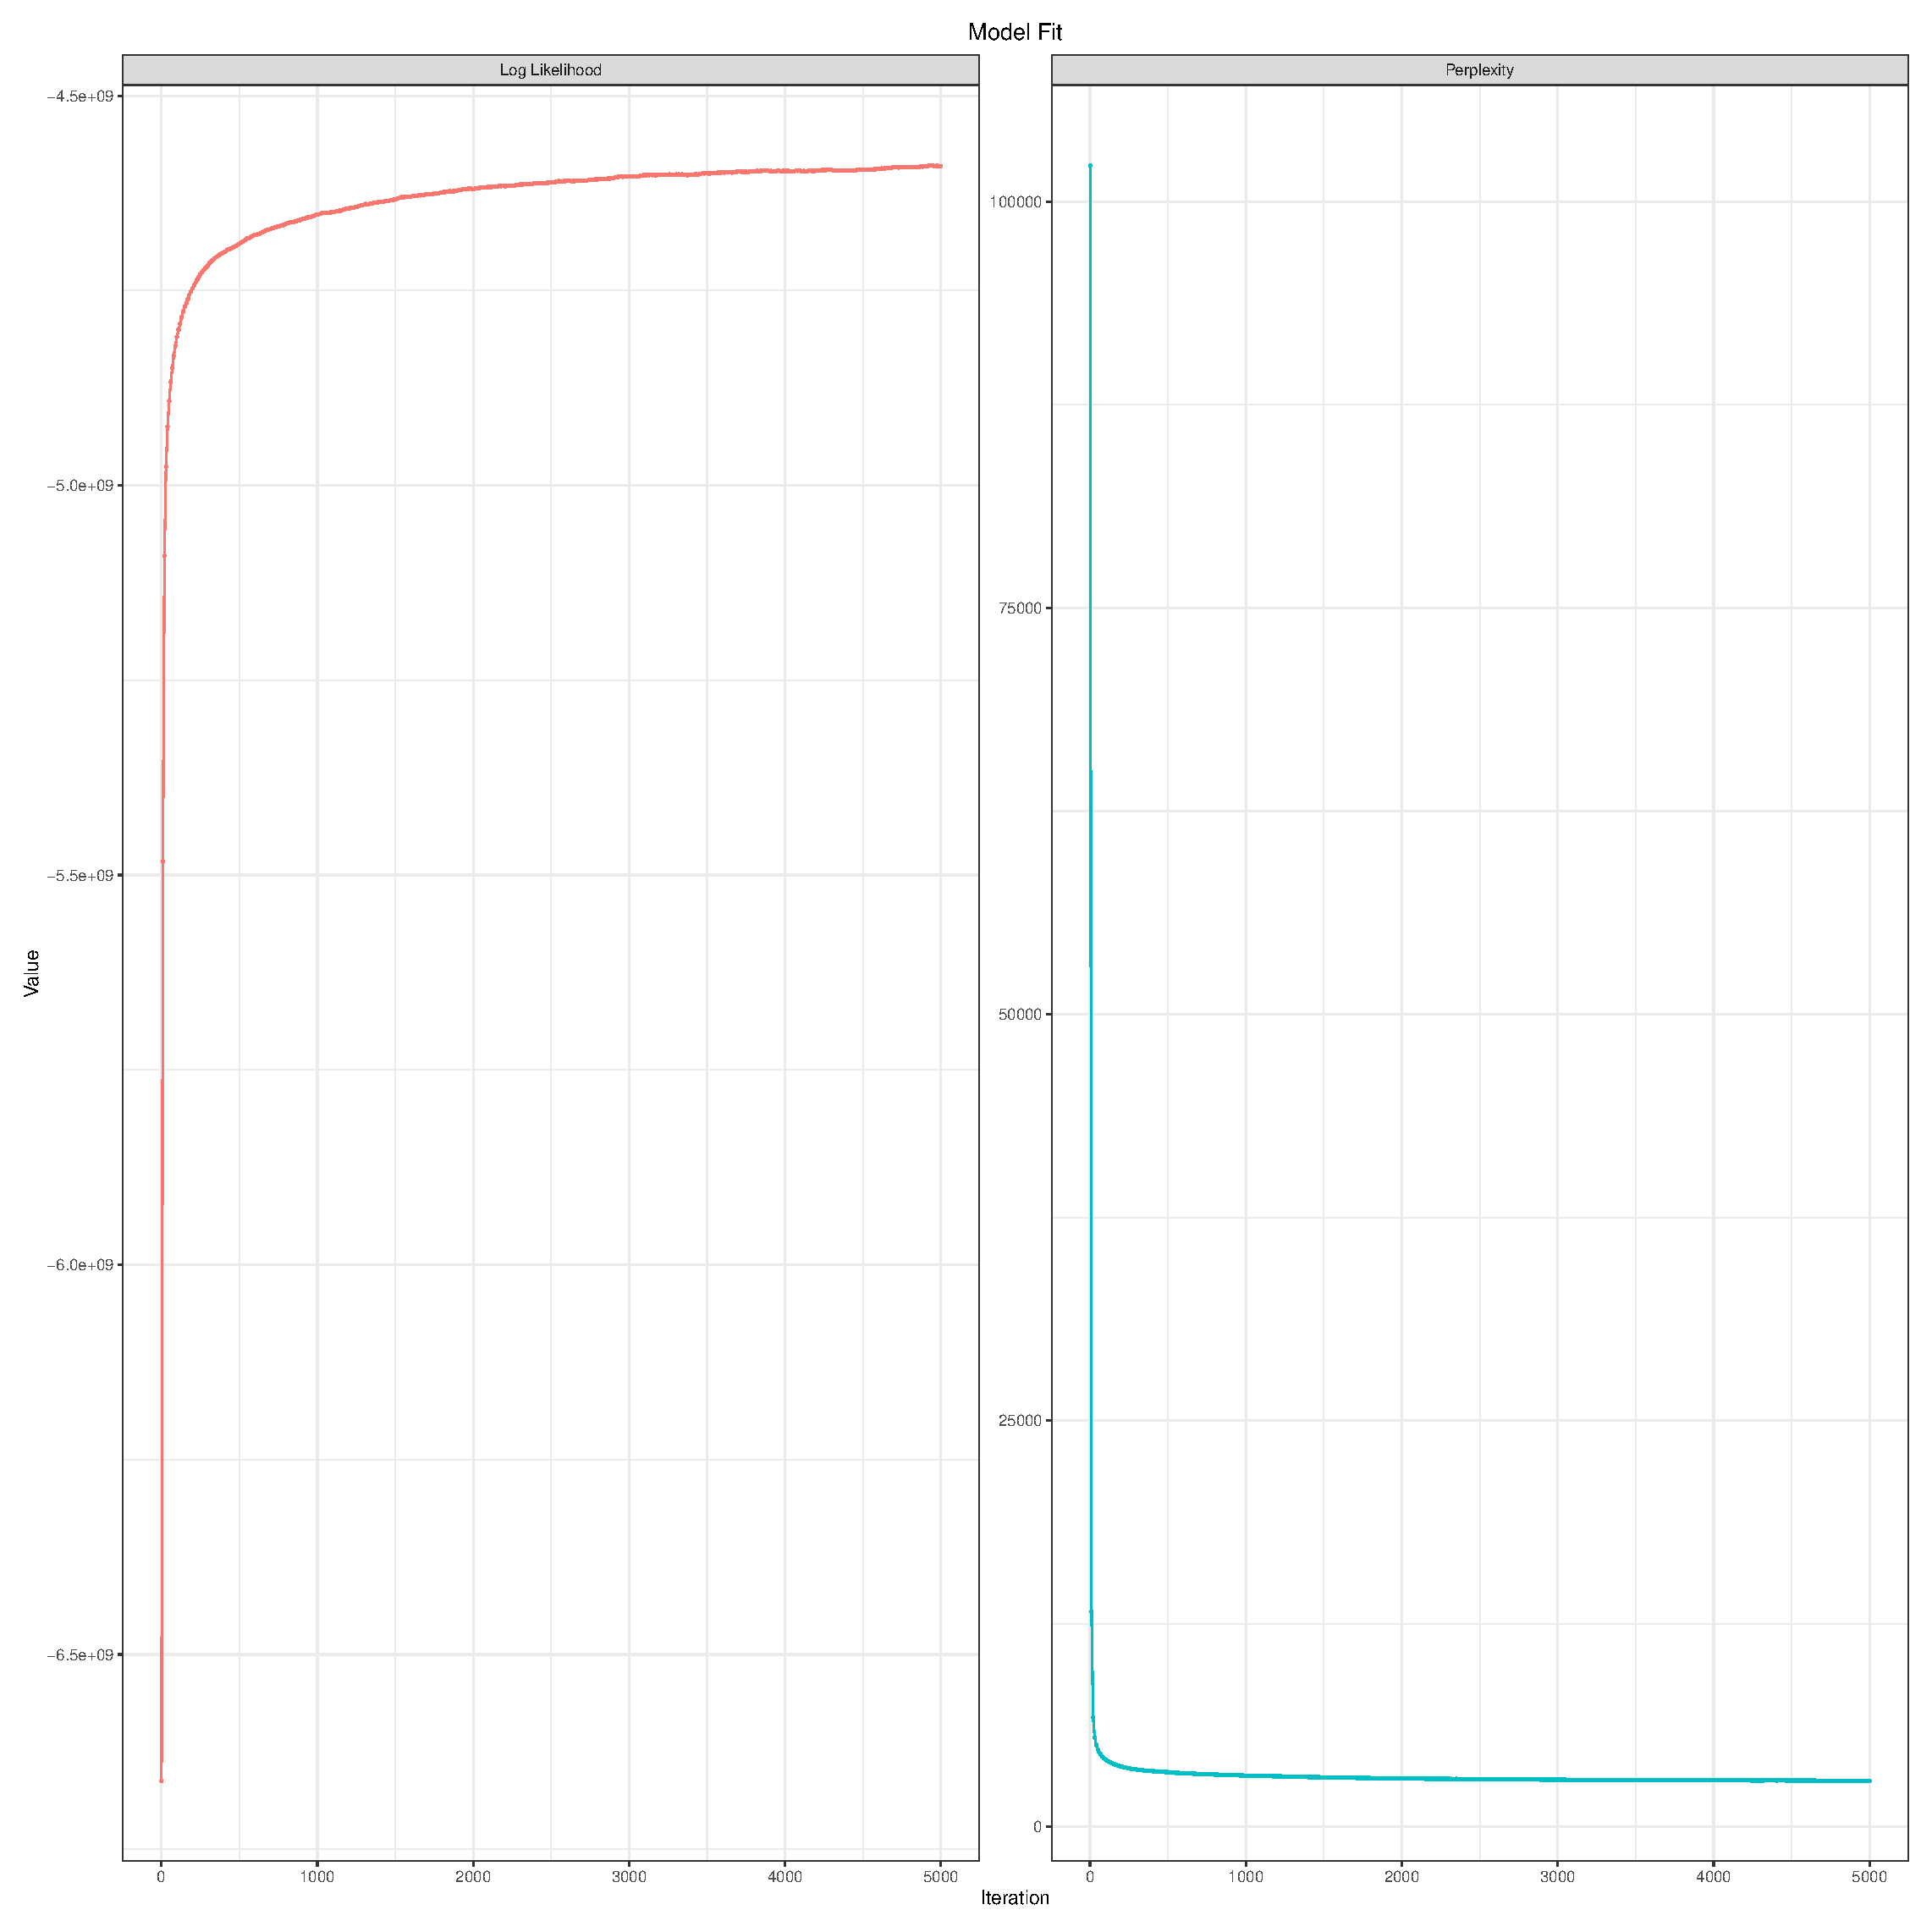
\includegraphics[width=1\linewidth]{figures/modelfit_djn_model.eps}
	\caption{Modelfit}
	\label{fig:modelfit}
\end{figure}

%Estimated Alpha
 \begin{figure}[H]
	\begin{center}
		\includegraphics[width=1.0\linewidth]{figures/alpha_djn_model.eps}
		\caption{Estimated alpha}
		\label{fig:alpha}
	\end{center}
\end{figure}

%Top-20 Words

 %% latex table generated in R 4.2.3 by xtable 1.8-4 package
% Wed Aug 23 21:41:09 2023

\begin{sidewaystable}[H]
	\centering
	\footnotesize
	\begin{tabular}{p{0.3cm}|p{1.4cm}|p{1.4cm}|p{1.4cm}|p{1.4cm}|p{1.4cm}|p{1.4cm}|p{1.4cm}|p{1.4cm}|p{1.4cm}|p{1.4cm}|p{1.4cm}|p{1.4cm}|p{1.4cm}}
	\caption{Top-20 words per keyword topic}\label{table:top_words}
	& energy & war & pandemic & labor shortage & supply chain & monetary policy & government spending & pent-up demand & demand-shift & profits & politics & debt & taxes \\ 
	\hline
	1 & price & russia [\checkmark] & coronavirus & job [\checkmark] & company & fed [\checkmark] & u.s & growth & price & share & president [\checkmark] & bank & tax [\checkmark] \\ 
	2 & oil [\checkmark] & ukraine [\checkmark] & pandemic [\checkmark] & labor [\checkmark] & price & rate & china & economist & inflation & company & biden [\checkmark] & debt [\checkmark] & plan \\ 
	3 & high & russian & covid-19 [\checkmark] & worker [\checkmark] & supply [\checkmark] & inflation & trade & expect & consumer [\checkmark] & profit [\checkmark] & house & bond & cost \\ 
	4 & market & u.s & u.s & wage [\checkmark] & cost & bank & tariff & inflation & rise & market & election & rate & pay \\ 
	5 & us & oil [1] & recovery [8] & rate & new & policy & bank & rise & increase & expect & trump [\checkmark] & market & income \\ 
	6 & gas [\checkmark] & price & new & unemployment & chain [\checkmark] & powell & economy & economy & high & group & democrats [\checkmark] & government [\checkmark] & increase \\ 
	7 & week & energy & vaccine & economy & sale & central & trump [11] & economic & sale & revenue & party [\checkmark] & central & make \\ 
	8 & barrel & gas [1] & economic & work & vehicle [9] & interest & stock & quarter & quarter & rise & senate [\checkmark] & currency & billion \\ 
	9 & energy & war [\checkmark] & case [\checkmark] & growth & demand [8] & federal [12] & market & eurozone & rate & million & state & dollar & new \\ 
	10 & demand [8] & country & economy & high & car & market & chinese & price & spending [7] & price & vote & billion & energy \\ 
	11 & rise & sanction & variant & market & high & economy & rate & high & food & plc & government [\checkmark] & interest & bill \\ 
	12 & crude [\checkmark] & europe & week & u.s & business & official & growth & fall & early & quarter & administration [7] & investor & climate \\ 
	13 & future & supply [5] & stimulus [7] & people & maker & reserve & global & datum & u.s & growth & u.s & economy & price \\ 
	14 & production & invasion [\checkmark] & omicron & last & increase & raise [13] & price & sector & index & high & republicans & country & government [7] \\ 
	15 & low & european & restriction & low & make & increase & rise & activity & cost & sale & support & u.s & change \\ 
	16 & day & global & government [7] & economist & industry & point & economic & index & last & penny & political & financial & include \\ 
	17 & fall & official & china & time & last & meeting & president [11] & bank & economist & analyst & new & high & use \\ 
	18 & supply [5] & world & lockdown [8] & rise & executive & economic & new & remain & expect & first & white & yield & state \\ 
	19 & expect & high & country & inflation & u.s & expect & inflation & survey & good & u.k & former & economic & benefit \\ 
	20 & analyst & government [7] & demand [8] & pay & production & high & investor & gdp & fall & fall & leader & fund & high \\ 
		\hline
	
	\end{tabular}
\end{sidewaystable}



%Change in Mean

\begin{figure}[H]
	\centering
	\includegraphics[width=0.7\linewidth, angle = 270]{figures/plot_change.eps}
	\caption{Change of mean proportions}
	\label{fig:change}
	\floatfoot{Note: The Figure shows the change in mean proportions since 2021 with the 95\% confidence intervals. To calculate the relative proportions only the topics with pre-specified keywords were considered, so that the sum of the proportions of all keyword topics equals 1. All other non-keyword topics were excluded. We organized the topics by following the code system provided by \cite{Andre.2023}.}
\end{figure}




\begin{sidewaysfigure}[H]
	\centering
	\includegraphics[width=0.7\linewidth, angle = 270]{figures/comparision.eps}
	\caption{Change of mean proportions}
	\label{fig:comparision}
\end{sidewaysfigure}

\begin{sidewaystable}[H]
\centering
\caption{Elliott, Rothenberg and Stock unit root test results}\label{table:ers}

\begin{tabular}{lcccc}
\toprule
\textbf{Variable} & \textbf{Statistic} & \textbf{Critical Value 1\%} & \textbf{Critical Value 5\%} & \textbf{Critical Value 10\%} \\
\midrule
Government Spending & 1.6 & 1.95 & 3.11 & 4.17 \\
Monetary Policy & 5.22 & 1.95 & 3.11 & 4.17 \\
Demand & 3.73 & 1.95 & 3.11 & 4.17 \\
Demand Shift & 5.3 & 1.95 & 3.11 & 4.17 \\
Supply Chain & 4.3 & 1.95 & 3.11 & 4.17 \\
Energy & 2.17 & 1.95 & 3.11 & 4.17 \\
Labor Shortage & 9.01 & 1.95 & 3.11 & 4.17 \\
Supply & 3.44 & 1.95 & 3.11 & 4.17 \\
Pandemic & 2.03 & 1.95 & 3.11 & 4.17 \\
Politics & 4.85 & 1.95 & 3.11 & 4.17 \\
War & 0.83 & 1.95 & 3.11 & 4.17 \\
Debt & 4.72 & 1.95 & 3.11 & 4.17 \\
Taxes & 3.09 & 1.95 & 3.11 & 4.17 \\
Profits & 6.34 & 1.95 & 3.11 & 4.17 \\
\bottomrule
\end{tabular}
\end{sidewaystable}



\newpage


%robustness Granger

\begin{table}[ht]
\centering
\caption{Narrative $\rightarrow$ Expectations Granger causality (level)}\label{tab:granger_level}

\begin{tabular}{lcc}
\toprule
\textbf{Narratives} & \textbf{One-Year Expectations} & \textbf{Three-Year Expectations} \\
& (Pr($>$F)) & (Pr($>$F)) \\
\midrule
\multicolumn{3}{l}{\textbf{Demand}} \\
\midrule
Government Spending & 0.23 & 0.38 \\
Monetary Policy & 0.68 & 0.01 ** \\
Demand Shift & 0.02 ** & $<$0.01 *** \\
Demand (residual) & 0.31 & 0.13 \\
\midrule
\multicolumn{3}{l}{\textbf{Supply}} \\
\midrule
Supply Chain & $<$0.01 *** & 0.03 ** \\
Energy & 0.83 & 0.26 \\
Labor Shortage & 0.15 & 0.12 \\
Supply (residual) & 0.18 & $<$0.01 *** \\
\midrule
\multicolumn{3}{l}{\textbf{Miscellaneous}} \\
\midrule
Pandemic & 0.76 & 0.94 \\
Politics & 0.15 & 0.10 * \\
War & 0.76 & 0.24 \\
Debt & 0.79 & 0.07 * \\
Taxes & 0.56 & 0.50 \\
Profits & $<$0.01 *** & $<$0.01 *** \\
\midrule
\bottomrule
\textit{Note:}  & \multicolumn{2}{r}{$^{*}$p$<$0.1; $^{**}$p$<$0.05; $^{***}$p$<$0.01} \\
\bottomrule
\end{tabular}
\end{table}

\newpage
\begin{table}[ht]
\centering
\caption{Narrative $\rightarrow$ Expectations Granger causality (differences)}\label{tab:granger}

\begin{tabular}{lcc}
\toprule
\textbf{Narratives} & \textbf{One-Year Expectations} & \textbf{Three-Year Expectations} \\
& (Pr($>$F)) & (Pr($>$F)) \\
\midrule
\multicolumn{3}{l}{\textbf{Demand}} \\
\midrule
Government Spending & 0.13 & 0.07 * \\
Monetary Policy & 0.55 & 0.29 \\
Demand Shift & 0.07 * & 0.27 \\
\midrule
\multicolumn{3}{l}{\textbf{Miscellaneous}} \\
\midrule
Demand (residual) & 0.80 & 0.84 \\
Supply (residual) & 0.22 & 0.12 \\
Pandemic & 0.68 & 0.65 \\
Politics & 0.67 & 0.98 \\
War & 0.50 & 0.12 \\
Debt & 0.03 ** & 0.88 \\
Taxes & 0.71 & 0.35 \\
Profits & 0.06 * & 0.08 * \\
\midrule
\multicolumn{3}{l}{\textbf{Supply}} \\
\midrule
Supply Chain & 0.02 ** & 0.24 \\
Energy & 0.91 & 0.35 \\
Labor Shortage & 0.16 & 0.73 \\
\midrule
\bottomrule
\textit{Note:}  & \multicolumn{2}{r}{$^{*}$p$<$0.1; $^{**}$p$<$0.05; $^{***}$p$<$0.01} \\
\bottomrule
\end{tabular}
\end{table}

\newpage


% heterogeneity

\begin{sidewaystable}[ht]
\centering
\caption{Income: Granger causality analysis (bHP-Filter)}\label{table:granger}

\begin{tabular}{lcccccc}
 \toprule
\textbf{Narratives} & \textbf{1-Year Low Income} & \textbf{3-Year Low Income} & \textbf{1-Year Mid Income} & \textbf{3-Year Mid Income} & \textbf{1-Year High Income} & \textbf{3-Year High Income} \\
\midrule
\multicolumn{7}{l}{\textbf{Demand}} \\
\midrule
Government Spending & 0.48 & 0.19 & 0.52 & 0.06 * & 0.73 & 0.28 \\
Monetary Policy & 0.50 & 0.63 & 0.44 & 0.15 & 0.10 * & 0.11 \\
Pent-up Demand & $<$0.01 *** & 0.25 & 0.13 & 0.15 & 0.05 * & 0.30 \\
Demand Shift & 0.33 & 0.18 & 0.50 & 0.74 & 0.59 & 0.49 \\
\midrule
\multicolumn{7}{l}{\textbf{Supply}} \\
\midrule
Supply Chain & $<$0.01 *** & 0.08 * & 0.02 ** & 0.32 & 0.01 ** & 0.08 * \\
Energy & 0.37 & 0.11 & 0.96 & 0.26 & 0.94 & 0.60 \\
Labor Shortage & 0.25 & 0.44 & 0.11 & 0.99 & 0.17 & 0.94 \\
\midrule
\multicolumn{7}{l}{\textbf{Miscellaneous}} \\
\midrule
Pandemic & 0.43 & 0.74 & 0.15 & 0.45 & 0.25 & 0.07 * \\
Politics & 0.85 & 0.81 & 0.57 & 0.33 & 0.88 & 0.56 \\
War & $<$0.01 *** & 0.10 * & 0.03 ** & 0.59 & 0.10 * & 0.25 \\
Debt & 0.36 & 0.74 & 0.35 & 0.95 & 0.27 & 0.36 \\
Taxes & 0.26 & 0.65 & 0.46 & 0.91 & 0.92 & 0.56 \\
Profits & $<$0.01 *** & 0.04 ** & 0.04 ** & 0.28 & 0.12 & $<$0.01 *** \\
\midrule
\bottomrule
\textit{Note:}  & \multicolumn{6}{r}{$^{*}$p$<$0.1; $^{**}$p$<$0.05; $^{***}$p$<$0.01} \\
\bottomrule
\end{tabular}
\end{sidewaystable}


\newpage

\begin{sidewaystable}[ht]
\centering
\caption{Education: Granger causality analysis (bHP-Filter)}\label{table:granger}

\begin{tabular}{lcccccc}
\toprule
\textbf{Narratives} & \textbf{1-Year Low Education} & \textbf{3-Year Low Education} & \textbf{1-Year Mid Education} & \textbf{3-Year Mid Education} & \textbf{1-Year High Education} & \textbf{3-Year High Education} \\
\midrule
\multicolumn{7}{l}{\textbf{Demand}} \\
\midrule
Government Spending & 0.07 * & 0.01 ** & 0.79 & $<$0.01 *** & 0.50 & 0.33 \\
Monetary Policy & 0.13 & 0.63 & 0.99 & 0.17 & 0.33 & 0.47 \\
Pent-up Demand & $<$0.01 *** & 0.71 & 0.06 * & 0.85 & 0.11 & 0.04 ** \\
Demand Shift & 0.04 ** & 0.11 & 0.83 & 0.54 & 0.47 & 0.61 \\
\midrule
\multicolumn{7}{l}{\textbf{Supply}} \\
\midrule
Supply Chain & $<$0.01 *** & 0.59 & 0.22 & 0.02 ** & $<$0.01 *** & $<$0.01 *** \\
Energy & 0.45 & 0.79 & 0.26 & 0.11 & 0.19 & 0.13 \\
Labor Shortage & 0.37 & 0.59 & 0.04 ** & 0.94 & 0.69 & 0.90 \\
\midrule
\multicolumn{7}{l}{\textbf{Miscellaneous}} \\
\midrule
Pandemic & 0.17 & 0.76 & 0.19 & 0.98 & 0.28 & 0.19 \\
Politics & 0.44 & 0.72 & 0.77 & 0.35 & 0.90 & 0.61 \\
War & $<$0.01 *** & 0.72 & $<$0.01 *** & 0.14 & 0.22 & 0.03 ** \\
Debt & 1.00 & 0.26 & 0.51 & 0.52 & 0.66 & 0.16 \\
Taxes & 0.06 * & 0.16 & 0.92 & 0.76 & 0.74 & 0.27 \\
Profits & $<$0.01 *** & 0.28 & 0.09 * & 0.07 * & 0.05 ** & $<$0.01 *** \\
\midrule
\bottomrule
\textit{Note:}  & \multicolumn{6}{r}{$^{*}$p$<$0.1; $^{**}$p$<$0.05; $^{***}$p$<$0.01} \\
\bottomrule
\end{tabular}
\end{sidewaystable}


\newpage

\begin{sidewaystable}[ht]
\centering
\caption{Age: Granger causality analysis (bHP-Filter)}\label{table:granger}

\begin{tabular}{lcccccc}
\toprule
\textbf{Narratives} & \textbf{1-Year Low Age} & \textbf{3-Year Low Age} & \textbf{1-Year Mid Age} & \textbf{3-Year Mid Age} & \textbf{1-Year High Age} & \textbf{3-Year High Age} \\
\midrule
\multicolumn{7}{l}{\textbf{Demand}} \\
\midrule
Government Spending & 0.15 & 0.34 & 0.21 & 0.01 ** & 0.46 & 0.01 ** \\
Monetary Policy & 0.73 & 0.58 & 0.16 & 0.72 & 0.44 & 0.12 \\
Pent-up Demand & $<$0.01 *** & 0.14 & 0.07 * & 0.56 & 0.45 & 0.67 \\
Demand Shift & 0.76 & 0.21 & 0.22 & 0.97 & 0.62 & 0.05 ** \\
\midrule
\multicolumn{7}{l}{\textbf{Supply}} \\
\midrule
Supply Chain & 0.08 * & 0.01 ** & $<$0.01 *** & $<$0.01 *** & 0.08 * & 0.05 ** \\
Energy & 0.54 & 0.23 & 0.31 & 0.70 & 0.48 & 0.10 * \\
Labor Shortage & 0.73 & 0.86 & 0.27 & 0.62 & 0.13 & 0.35 \\
\midrule
\multicolumn{7}{l}{\textbf{Miscellaneous}} \\
\midrule
Pandemic & 0.13 & 0.14 & 0.89 & 0.35 & 0.22 & $<$0.01 *** \\
Politics & 0.53 & 0.64 & 0.95 & 0.31 & 0.50 & 0.95 \\
War & 0.02 ** & $<$0.01 *** & 0.15 & 0.06 * & 0.04 ** & 0.75 \\
Debt & 0.08 * & 0.81 & 0.93 & 0.46 & 0.45 & 0.92 \\
Taxes & 0.48 & 0.07 * & 0.52 & 0.92 & 0.28 & 0.76 \\
Profits & 0.22 & 0.01 ** & 0.02 ** & $<$0.01 *** & 0.07 * & 0.09 * \\
\midrule
\bottomrule
\textit{Note:}  & \multicolumn{6}{r}{$^{*}$p$<$0.1; $^{**}$p$<$0.05; $^{***}$p$<$0.01} \\
\bottomrule
\end{tabular}
\end{sidewaystable}


\newpage
\begin{sidewaystable}[ht]
\centering
\caption{Numeracy: Granger causality analysis (bHP-Filter)}\label{table:granger}

\begin{tabular}{lcccc}
\toprule
\textbf{Narratives} & \textbf{1-Year Low Numeracy} & \textbf{3-Year Low Numeracy} & \textbf{1-Year High Numeracy} & \textbf{3-Year High Numeracy} \\
\midrule
\multicolumn{5}{l}{\textbf{Demand}} \\
\midrule
Government Spending & 0.69 & 0.05 * & 0.54 & 0.04 ** \\
Monetary Policy & 0.41 & 0.36 & 0.17 & 0.38 \\
Pent-up Demand & 0.27 & 0.92 & 0.01 ** & 0.84 \\
Demand Shift & 0.96 & 0.42 & 0.30 & 0.31 \\
\midrule
\multicolumn{5}{l}{\textbf{Supply}} \\
\midrule
Supply Chain & 0.04 ** & 0.44 & $<$0.01 *** & 0.44 \\
Energy & 0.81 & 0.20 & 0.96 & 0.16 \\
Labor Shortage & 0.13 & 0.98 & 0.09 * & 0.92 \\
\midrule
\multicolumn{5}{l}{\textbf{Miscellaneous}} \\
\midrule
Pandemic & 0.16 & 0.89 & 0.36 & 0.71 \\
Politics & 0.36 & 0.41 & 0.57 & 0.47 \\
War & $<$0.01 *** & 0.02 ** & 0.10 & 0.05 ** \\
Debt & 0.19 & 0.30 & 0.35 & 0.20 \\
Taxes & 0.30 & 0.22 & 0.65 & 0.18 \\
Profits & 0.04 ** & 0.10 & 0.12 & 0.10 * \\
\midrule
\bottomrule
\textit{Note:}  & \multicolumn{4}{r}{$^{*}$p$<$0.1; $^{**}$p$<$0.05; $^{***}$p$<$0.01} \\
\bottomrule
\end{tabular}
\end{sidewaystable}




% Irfs complete

\newpage
\begin{sidewaysfigure}[H]
	\centering
	\captionsetup{font=footnotesize}
	\begin{subfigure}{00.24\textwidth}
		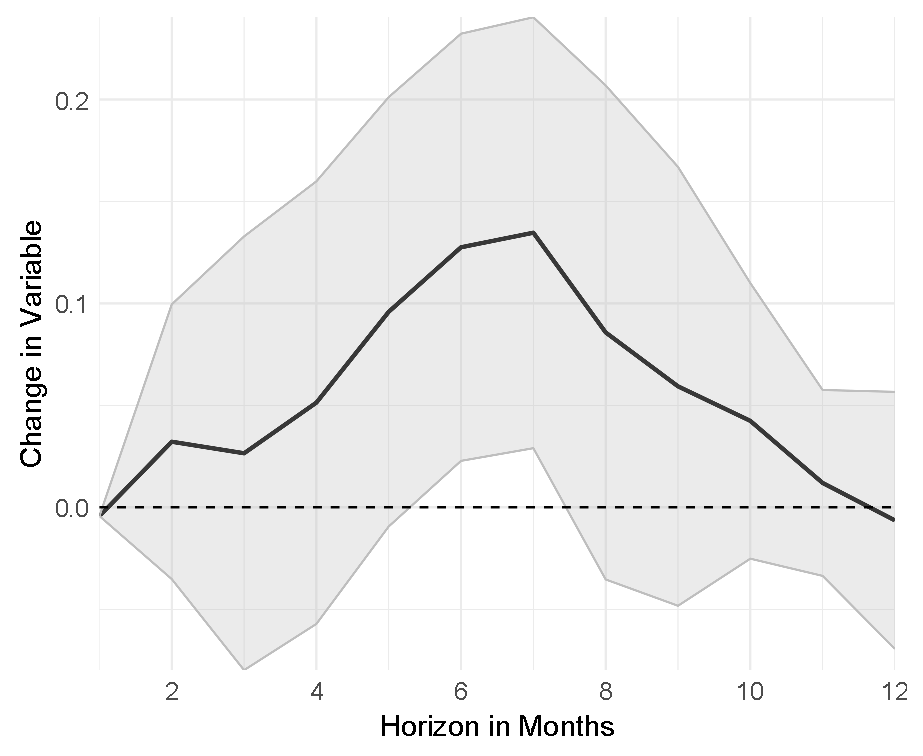
\includegraphics[width=0.8\textwidth]{output/lp/baseline/bHP/government_spending/government_spendingonexpectations1y_djn.eps}
		\caption{Government spending on 1-year expectations}
	\end{subfigure}
	\begin{subfigure}{00.24\textwidth}
		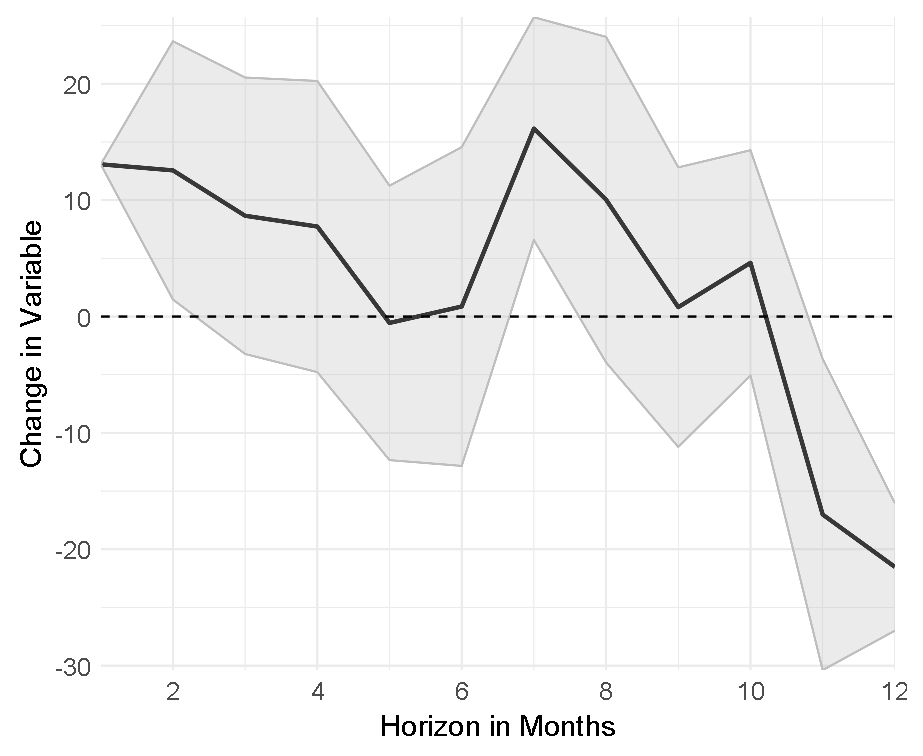
\includegraphics[width=0.8\textwidth]{output/lp/baseline/bHP/government_spending/government_spendingonexpectations3y_djn.eps}
		\caption{Government spending on 3-year expectations}
	\end{subfigure}
	\begin{subfigure}{00.24\textwidth}
	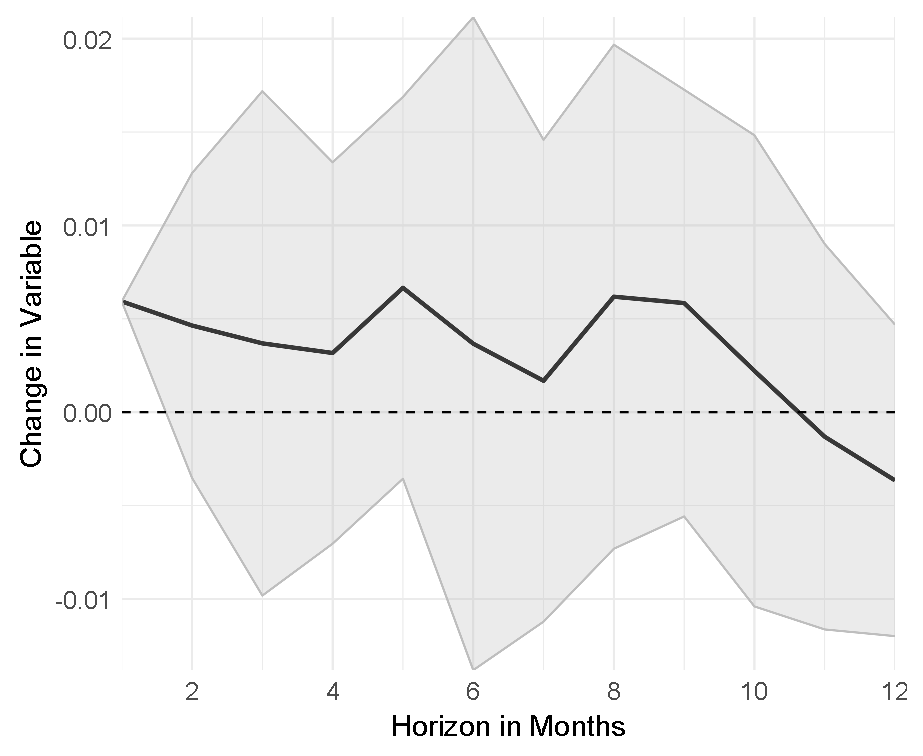
\includegraphics[width=0.8\textwidth]{output/lp/baseline/bHP/government_spending/government_spendingoninflation_djn.eps}
	\caption{Government spending on CPI inflation}
	\end{subfigure}
	\begin{subfigure}{00.24\textwidth}
		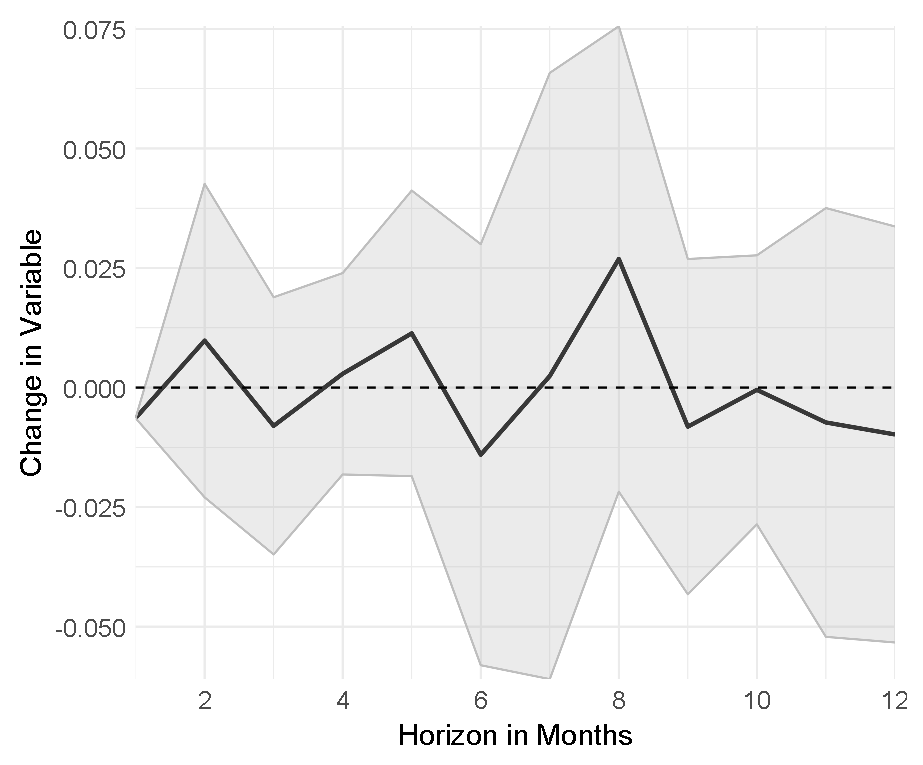
\includegraphics[width=0.8\textwidth]{output/lp/baseline/bHP/government_spending/government_spendingoneconac_djn.eps}
		\caption{Government spending on economic activity}
	\end{subfigure}
	\begin{subfigure}{00.24\textwidth}
		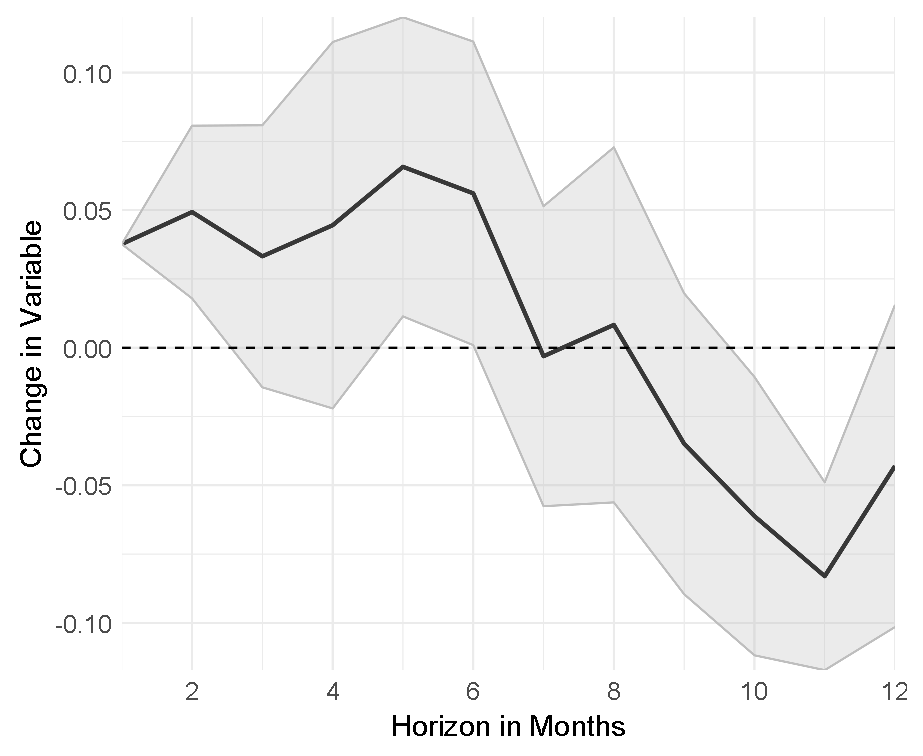
\includegraphics[width=0.8\textwidth]{output/lp/baseline/bHP/monetary_policy/monetary_policyonexpectations1y_djn.eps}
		\caption{Monetary policy on 1-year expectations}
	\end{subfigure}
	\begin{subfigure}{00.24\textwidth}
		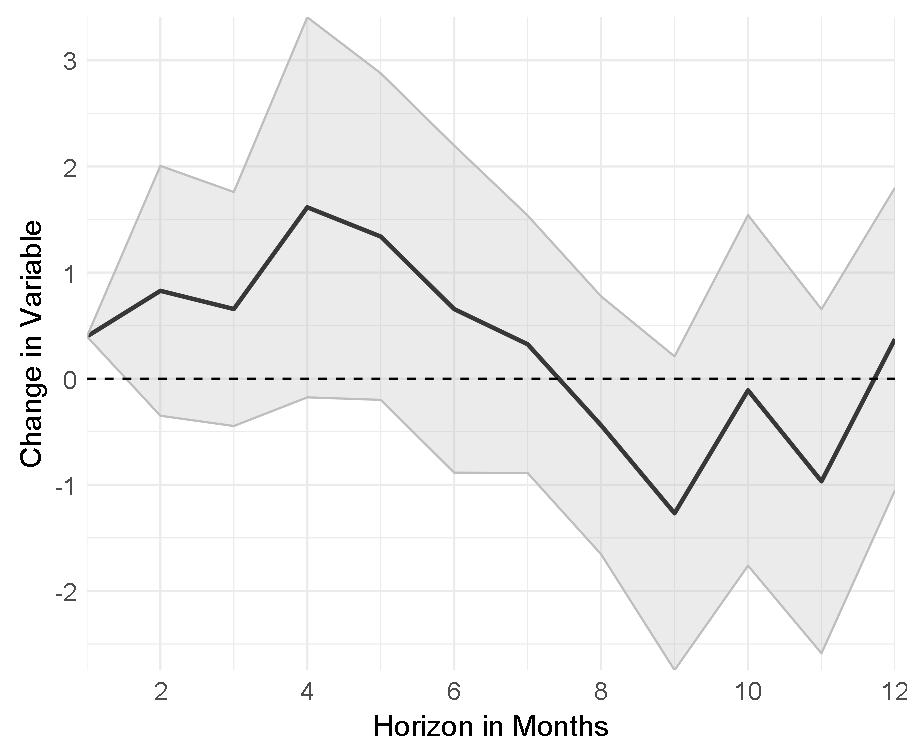
\includegraphics[width=0.8\textwidth]{output/lp/baseline/bHP/monetary_policy/monetary_policyonexpectations3y_djn.eps}
		\caption{Monetary policy on 3-year expectations}
	\end{subfigure}
	\begin{subfigure}{00.24\textwidth}
		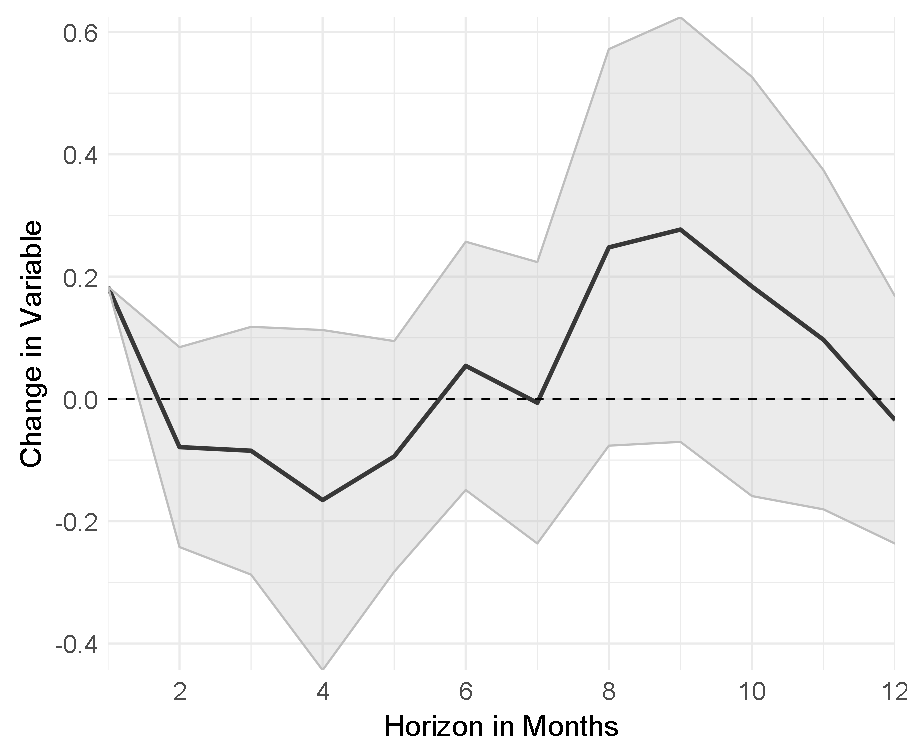
\includegraphics[width=0.8\textwidth]{output/lp/baseline/bHP/monetary_policy/monetary_policyoninflation_djn.eps}
		\caption{Monetary policy on CPI inflation}
	\end{subfigure}
	\begin{subfigure}{00.24\textwidth}
		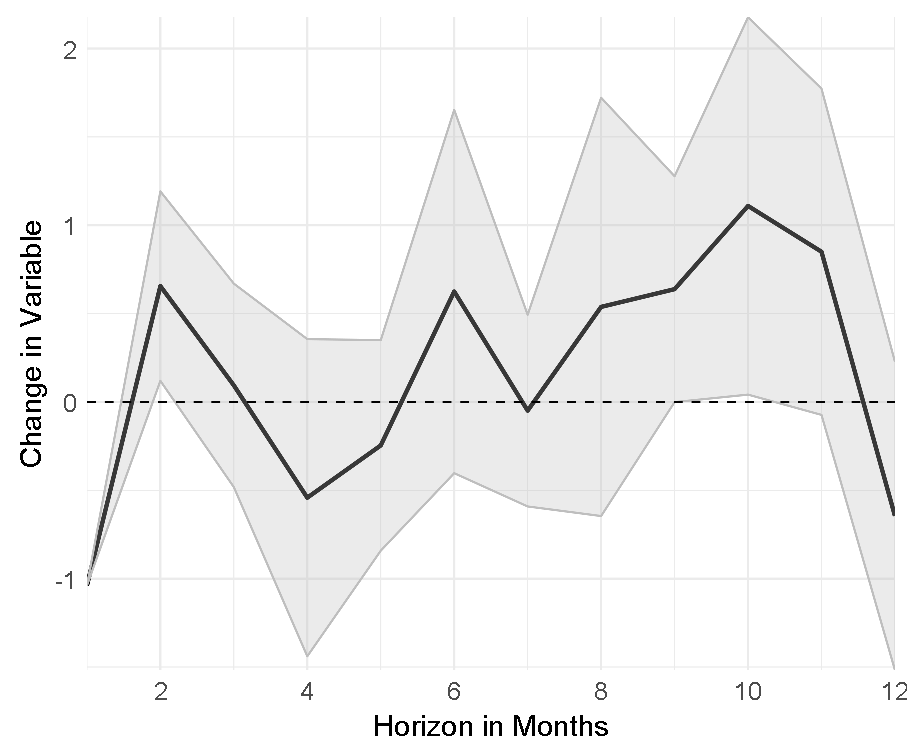
\includegraphics[width=0.8\textwidth]{output/lp/baseline/bHP/monetary_policy/monetary_policyoneconac_djn.eps}
		\caption{Monetary policy on economic activity}
	\end{subfigure}
	\begin{subfigure}{00.24\textwidth}
		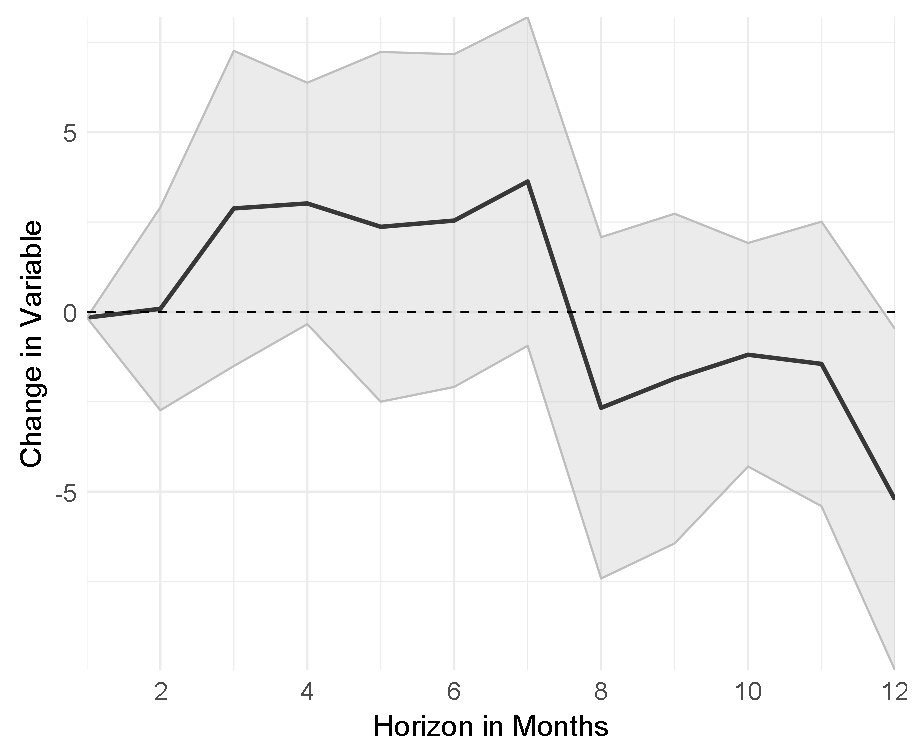
\includegraphics[width=0.8\textwidth]{output/lp/baseline/bHP/demand/demandonexpectations1y_djn.eps}
		\caption{Demand (residual) on 1-year expectations}
	\end{subfigure}
	\begin{subfigure}{00.24\textwidth}
		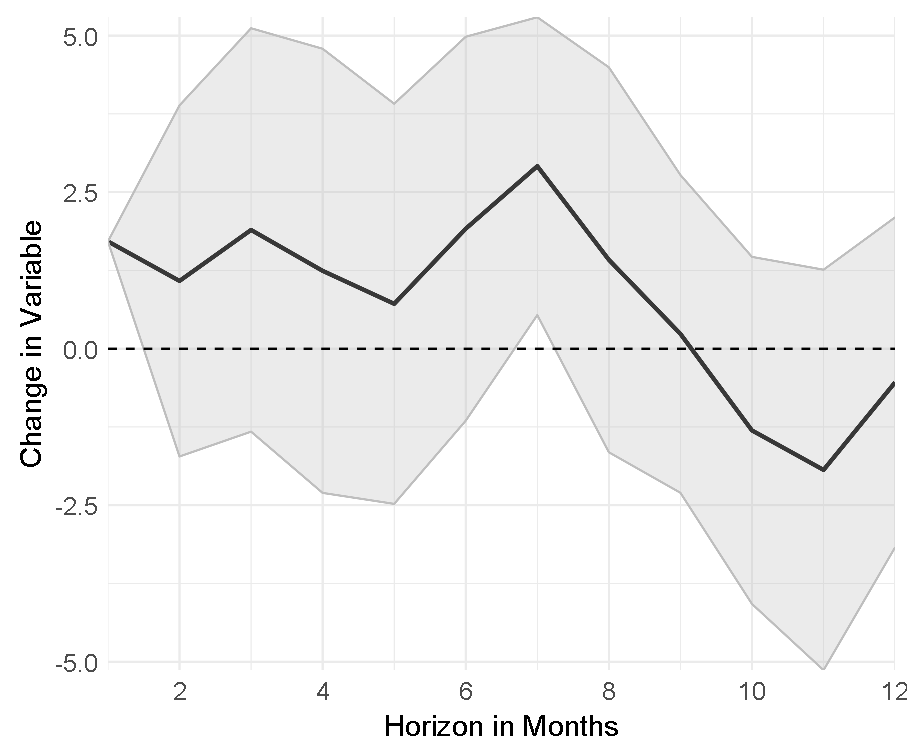
\includegraphics[width=0.8\textwidth]{output/lp/baseline/bHP/demand/demandonexpectations3y_djn.eps}
		\caption{Demand (residual) on 3-year expectations}
	\end{subfigure}
	\begin{subfigure}{00.24\textwidth}
		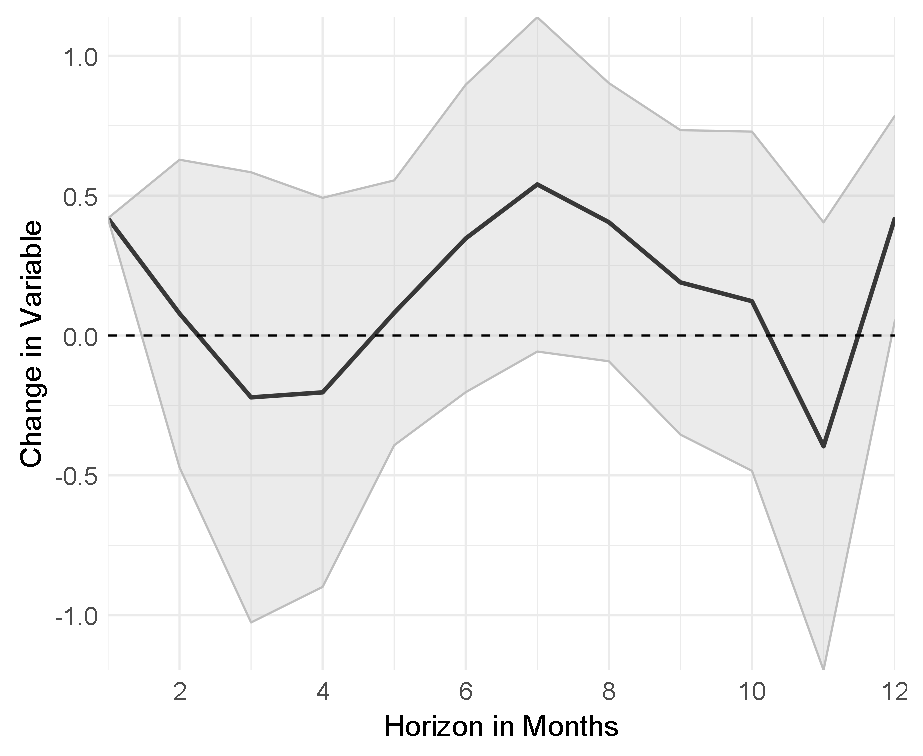
\includegraphics[width=0.8\textwidth]{output/lp/baseline/bHP/demand/demandoninflation_djn.eps}
		\caption{Demand (residual) on CPI inflation}
	\end{subfigure}
	\begin{subfigure}{00.24\textwidth}
		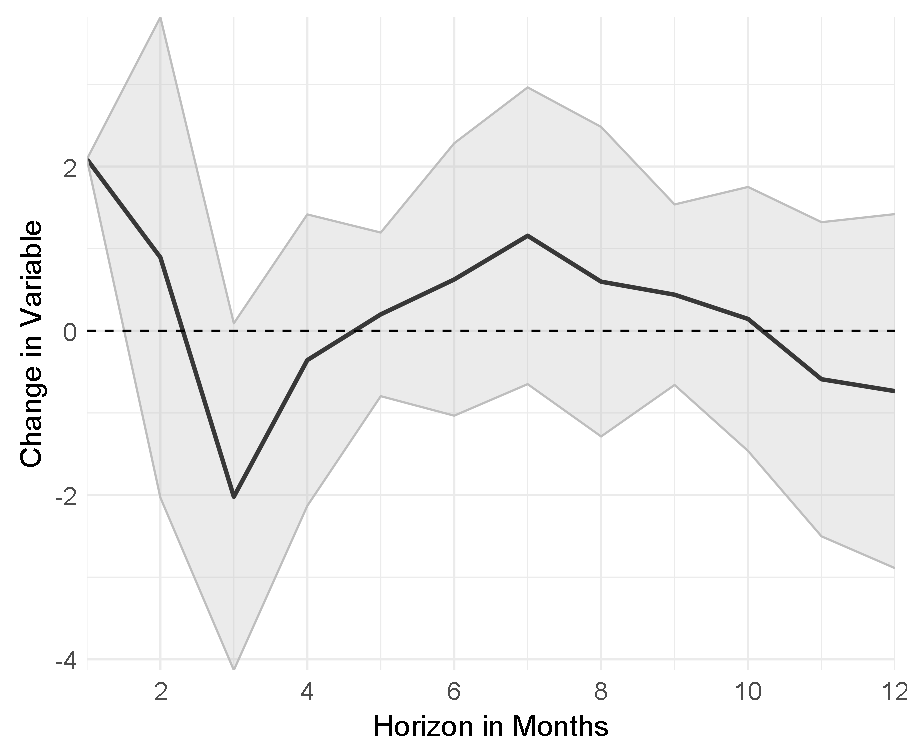
\includegraphics[width=0.8\textwidth]{output/lp/baseline/bHP/demand/demandoneconac_djn.eps}
		\caption{Demand (residual) on economic activity}
	\end{subfigure}
	\begin{subfigure}{00.24\textwidth}
		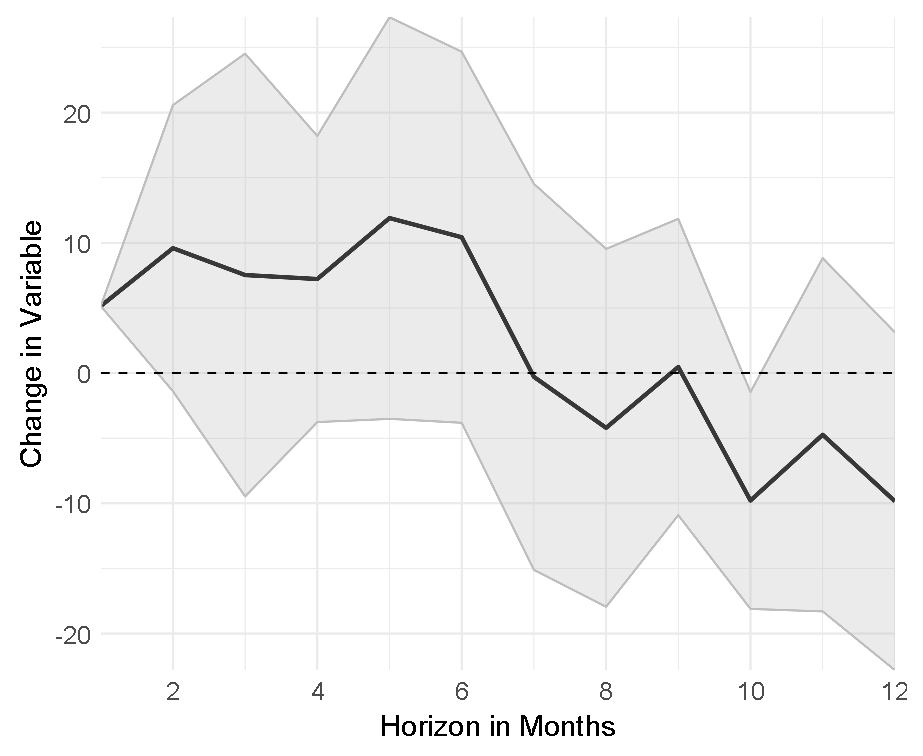
\includegraphics[width=0.8\textwidth]{output/lp/baseline/bHP/demand_shift/demand_shiftonexpectations1y_djn.eps}
		\caption{Demand shift on 1-year expectations}
	\end{subfigure}
	\begin{subfigure}{00.24\textwidth}
		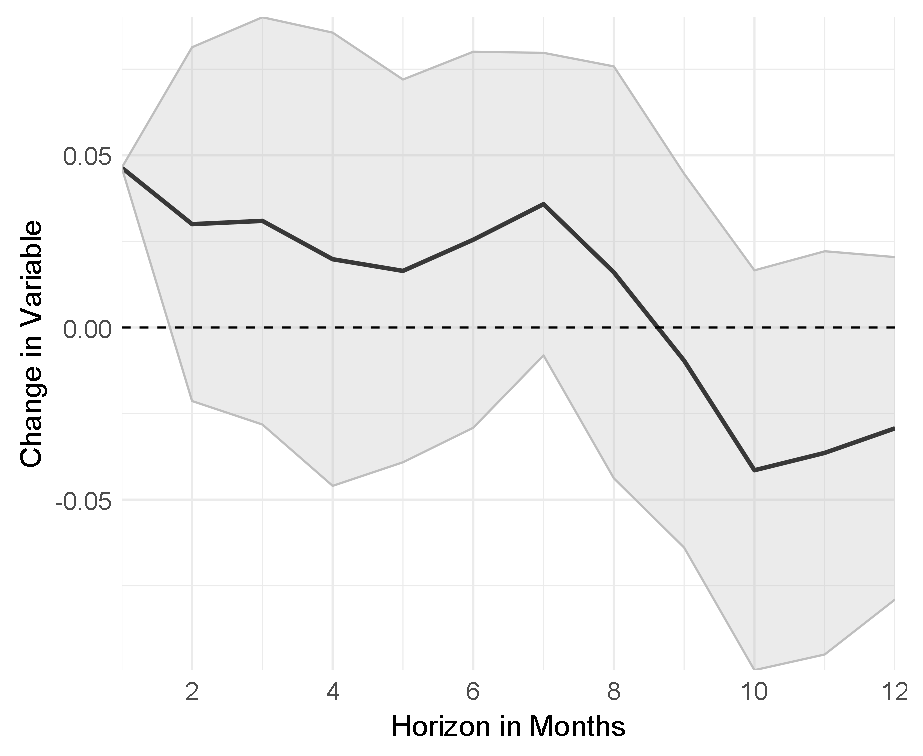
\includegraphics[width=0.8\textwidth]{output/lp/baseline/bHP/demand_shift/demand_shiftonexpectations3y_djn.eps}
		\caption{Demand shift on 3-year expectations}
	\end{subfigure}
	\begin{subfigure}{00.24\textwidth}
		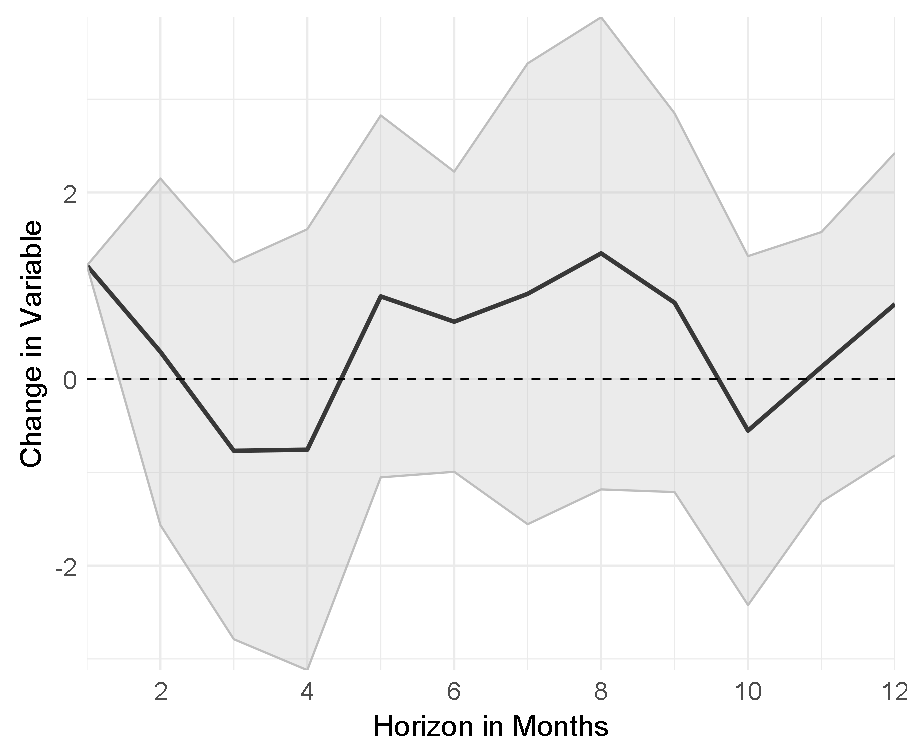
\includegraphics[width=0.8\textwidth]{output/lp/baseline/bHP/demand_shift/demand_shiftoninflation_djn.eps}
		\caption{Demand shift on CPI inflation}
	\end{subfigure}
	\begin{subfigure}{00.24\textwidth}
		\includegraphics[width=0.8\textwidth]{output/lp/baseline/bHP/demand_shift/demand_shiftoneconac_djn.eps}
		\caption{Demand shift on economic activity}
	\end{subfigure}
	\caption{Demand narratives' impulse responses}
	\label{fig:irf_1}
\end{sidewaysfigure}

\newpage
\begin{sidewaysfigure}[H]
	\centering
	\captionsetup{font=footnotesize}
	\begin{subfigure}{00.24\textwidth}
		\includegraphics[width=0.8\textwidth]{output/lp/baseline/bHP/supply_chain/supply_chainonexpectations1y_djn.eps}
		\caption{Supply chain on 1-year expectations}
	\end{subfigure}
	\begin{subfigure}{00.24\textwidth}
		\includegraphics[width=0.8\textwidth]{output/lp/baseline/bHP/supply_chain/supply_chainonexpectations3y_djn.eps}
		\caption{Supply chain on 3-year expectations}
	\end{subfigure}
	\begin{subfigure}{00.24\textwidth}
		\includegraphics[width=0.8\textwidth]{output/lp/baseline/bHP/supply_chain/supply_chainoninflation_djn.eps}
		\caption{Supply chain on CPI inflation}
	\end{subfigure}
	\begin{subfigure}{00.24\textwidth}
		\includegraphics[width=0.8\textwidth]{output/lp/baseline/bHP/supply_chain/supply_chainoneconac_djn.eps}
		\caption{Supply chain on economic activity}
	\end{subfigure}
	\begin{subfigure}{00.24\textwidth}
		\includegraphics[width=0.8\textwidth]{output/lp/baseline/bHP/energy/energyonexpectations1y_djn.eps}
		\caption{Energy on 1-year expectations}
	\end{subfigure}
	\begin{subfigure}{00.24\textwidth}
		\includegraphics[width=0.8\textwidth]{output/lp/baseline/bHP/energy/energyonexpectations3y_djn.eps}
		\caption{Energy on 3-year expectations}
	\end{subfigure}
	\begin{subfigure}{00.24\textwidth}
		\includegraphics[width=0.8\textwidth]{output/lp/baseline/bHP/energy/energyoninflation_djn.eps}
		\caption{Energy on CPI inflation}
	\end{subfigure}
	\begin{subfigure}{00.24\textwidth}
		\includegraphics[width=0.8\textwidth]{output/lp/baseline/bHP/energy/energyoneconac_djn.eps}
		\caption{Energy on economic activity}
	\end{subfigure}
	\begin{subfigure}{00.24\textwidth}
		\includegraphics[width=0.8\textwidth]{output/lp/baseline/bHP/labor_shortage/labor_shortageonexpectations1y_djn.eps}
		\caption{Labor shortage on 1-year expectations}
	\end{subfigure}
	\begin{subfigure}{00.24\textwidth}
		\includegraphics[width=0.8\textwidth]{output/lp/baseline/bHP/labor_shortage/labor_shortageonexpectations3y_djn.eps}
		\caption{Labor shortage on 3-year expectations}
	\end{subfigure}
	\begin{subfigure}{00.24\textwidth}
		\includegraphics[width=0.8\textwidth]{output/lp/baseline/bHP/labor_shortage/labor_shortageoninflation_djn.eps}
		\caption{Labor shortage on CPI inflation}
	\end{subfigure}
	\begin{subfigure}{00.24\textwidth}
		\includegraphics[width=0.8\textwidth]{output/lp/baseline/bHP/labor_shortage/labor_shortageoneconac_djn.eps}
		\caption{Labor shortage on economic activity}
	\end{subfigure}
		\begin{subfigure}{00.24\textwidth}
		\includegraphics[width=0.8\textwidth]{output/lp/baseline/bHP/supply/supplyonexpectations1y_djn.eps}
		\caption{Supply (residual) on 1-year expectations}
	\end{subfigure}
	\begin{subfigure}{00.24\textwidth}
		\includegraphics[width=0.8\textwidth]{output/lp/baseline/bHP/supply/supplyonexpectations3y_djn.eps}
		\caption{Supply (residual) on 3-year expectations}
	\end{subfigure}
	\begin{subfigure}{00.24\textwidth}
		\includegraphics[width=0.8\textwidth]{output/lp/baseline/bHP/supply/supplyoninflation_djn.eps}
		\caption{Supply (residual) on CPI inflation}
	\end{subfigure}
	\begin{subfigure}{00.24\textwidth}
		\includegraphics[width=0.8\textwidth]{output/lp/baseline/bHP/supply/supplyoneconac_djn.eps}
		\caption{Supply (residual) on economic activity}
	\end{subfigure}
	\caption{Supply narratives' impulse responses (bHP)}
	\label{fig:irf_2}
\end{sidewaysfigure}

\newpage
\begin{sidewaysfigure}[H]
	\centering
	\captionsetup{font=footnotesize}
	\begin{subfigure}{00.24\textwidth}
		\includegraphics[width=0.8\textwidth]{output/lp/baseline/bHP/pandemic/pandemiconexpectations1y_djn.eps}
		\caption{Pandemic on 1-year expectations}
	\end{subfigure}
	\begin{subfigure}{00.24\textwidth}
		\includegraphics[width=0.8\textwidth]{output/lp/baseline/bHP/pandemic/pandemiconexpectations3y_djn.eps}
		\caption{Pandemic on 3-year expectations}
	\end{subfigure}
	\begin{subfigure}{00.24\textwidth}
		\includegraphics[width=0.8\textwidth]{output/lp/baseline/bHP/pandemic/pandemiconinflation_djn.eps}
		\caption{Pandemic on CPI inflation}
	\end{subfigure}
	\begin{subfigure}{00.24\textwidth}
		\includegraphics[width=0.8\textwidth]{output/lp/baseline/bHP/pandemic/pandemiconeconac_djn.eps}
		\caption{Pandemic on economic activity}
	\end{subfigure}
	\begin{subfigure}{00.24\textwidth}
		\includegraphics[width=0.8\textwidth]{output/lp/baseline/bHP/politics/politicsonexpectations1y_djn.eps}
		\caption{Politics on 1-year expectations}
	\end{subfigure}
	\begin{subfigure}{00.24\textwidth}
		\includegraphics[width=0.8\textwidth]{output/lp/baseline/bHP/politics/politicsonexpectations3y_djn.eps}
		\caption{Politics on 3-year expectations}
	\end{subfigure}
	\begin{subfigure}{00.24\textwidth}
		\includegraphics[width=0.8\textwidth]{output/lp/baseline/bHP/politics/politicsoninflation_djn.eps}
		\caption{Politics on CPI inflation}
	\end{subfigure}
	\begin{subfigure}{00.24\textwidth}
		\includegraphics[width=0.8\textwidth]{output/lp/baseline/bHP/politics/politicsoneconac_djn.eps}
		\caption{Politics on economic activity}
	\end{subfigure}
	\begin{subfigure}{00.24\textwidth}
		\includegraphics[width=0.8\textwidth]{output/lp/baseline/bHP/war/waronexpectations1y_djn.eps}
		\caption{War on 1-year expectations}
	\end{subfigure}
	\begin{subfigure}{00.24\textwidth}
		\includegraphics[width=0.8\textwidth]{output/lp/baseline/bHP/war/waronexpectations3y_djn.eps}
		\caption{War on 3-year expectations}
	\end{subfigure}
	\begin{subfigure}{00.24\textwidth}
		\includegraphics[width=0.8\textwidth]{output/lp/baseline/bHP/war/waroninflation_djn.eps}
		\caption{War on CPI inflation}
	\end{subfigure}
	\begin{subfigure}{00.24\textwidth}
		\includegraphics[width=0.8\textwidth]{output/lp/baseline/bHP/war/waroneconac_djn.eps}
		\caption{War on economic activity}
	\end{subfigure}
	\begin{subfigure}{00.24\textwidth}
		\includegraphics[width=0.8\textwidth]{output/lp/baseline/bHP/debt/debtonexpectations1y_djn.eps}
		\caption{Debt on 1-year expectations}
	\end{subfigure}
	\begin{subfigure}{00.24\textwidth}
		\includegraphics[width=0.8\textwidth]{output/lp/baseline/bHP/debt/debtonexpectations3y_djn.eps}
		\caption{Debt on 3-year expectations}
	\end{subfigure}
	\begin{subfigure}{00.24\textwidth}
		\includegraphics[width=0.8\textwidth]{output/lp/baseline/bHP/debt/debtoninflation_djn.eps}
		\caption{Debt on CPI inflation}
	\end{subfigure}
	\begin{subfigure}{00.24\textwidth}
		\includegraphics[width=0.8\textwidth]{output/lp/baseline/bHP/debt/debtoneconac_djn.eps}
		\caption{Debt on economic activity}
	\end{subfigure}
	\caption{Miscellaneous narratives' impulse responses (bHP)}
	\label{fig:irf_3}
\end{sidewaysfigure}

\newpage
\begin{sidewaysfigure}[H]
	\centering
	\captionsetup{font=footnotesize}
	\begin{subfigure}{00.24\textwidth}
		\includegraphics[width=0.8\textwidth]{output/lp/baseline/bHP/taxes/taxesonexpectations1y_djn.eps}
		\caption{Taxes on 1-year expectations}
	\end{subfigure}
	\begin{subfigure}{00.24\textwidth}
		\includegraphics[width=0.8\textwidth]{output/lp/baseline/bHP/taxes/taxesonexpectations3y_djn.eps}
		\caption{Taxes on 3-year expectations}
	\end{subfigure}
	\begin{subfigure}{00.24\textwidth}
		\includegraphics[width=0.8\textwidth]{output/lp/baseline/bHP/taxes/taxesoninflation_djn.eps}
		\caption{Taxes on CPI inflation}
	\end{subfigure}
	\begin{subfigure}{00.24\textwidth}
		\includegraphics[width=0.8\textwidth]{output/lp/baseline/bHP/taxes/taxesoneconac_djn.eps}
		\caption{Taxes on economic activity}
	\end{subfigure}
	\begin{subfigure}{00.24\textwidth}
		\includegraphics[width=0.8\textwidth]{output/lp/baseline/bHP/profits/profitsonexpectations1y_djn.eps}
		\caption{Profits on 1-year expectations}
	\end{subfigure}
	\begin{subfigure}{00.24\textwidth}
		\includegraphics[width=0.8\textwidth]{output/lp/baseline/bHP/profits/profitsonexpectations3y_djn.eps}
		\caption{Profits on 3-year expectations}
	\end{subfigure}
	\begin{subfigure}{00.24\textwidth}
		\includegraphics[width=0.8\textwidth]{output/lp/baseline/bHP/profits/profitsoninflation_djn.eps}
		\caption{Profits on CPI inflation}
	\end{subfigure}
	\begin{subfigure}{00.24\textwidth}
		\includegraphics[width=0.8\textwidth]{output/lp/baseline/bHP/profits/profitsoneconac_djn.eps}
		\caption{Profits on economic activity}
	\end{subfigure}
	\caption{Miscellaneous narratives' impulse responses (bHP)}
	\label{fig:irf_4}
\end{sidewaysfigure}



\newpage

%Robustness IRF



\begin{figure}[H]
	\centering
	\captionsetup{font=footnotesize}
	\begin{subfigure}{00.32\textwidth}
	\includegraphics[width=1\textwidth]{output/lp/baseline/level/government_spending/government_spendingonexpectations1y_djn.eps}
	\caption{Government spending on 1-year}
\end{subfigure}
\begin{subfigure}{00.32\textwidth}
	\includegraphics[width=1\textwidth]{output/lp/baseline/level/monetary_policy/monetary_policyonexpectations3y_djn.eps}
	\caption{Monetary policy on 3-year}
\end{subfigure}
\begin{subfigure}{00.32\textwidth}
	\includegraphics[width=1\textwidth]{output/lp/baseline/level/supply_chain/supply_chainonexpectations1y_djn.eps}
	\caption{Supply chain on 1-year}
\end{subfigure}
\begin{subfigure}{00.32\textwidth}
	\includegraphics[width=1\textwidth]{output/lp/baseline/level/pandemic/pandemiconexpectations1y_djn.eps}
	\caption{Pandemic on 1-year}
\end{subfigure}
\begin{subfigure}{00.32\textwidth}
	\includegraphics[width=1\textwidth]{output/lp/baseline/level/politics/politicsonexpectations3y_djn.eps}
	\caption{Politics on 3-year}
\end{subfigure}
\begin{subfigure}{00.32\textwidth}
	\includegraphics[width=1\textwidth]{output/lp/baseline/level/war/waronexpectations1y_djn.eps}
	\caption{War on 1-year}
\end{subfigure}
\begin{subfigure}{00.32\textwidth}
	\includegraphics[width=1\textwidth]{output/lp/baseline/level/war/waronexpectations3y_djn.eps}
	\caption{War on 3-year}
\end{subfigure}
\begin{subfigure}{00.32\textwidth}
	\includegraphics[width=1\textwidth]{output/lp/baseline/level/profits/profitsonexpectations1y_djn.eps}
	\caption{Profits on 1-year}
\end{subfigure}
\begin{subfigure}{00.32\textwidth}
	\includegraphics[width=1\textwidth]{output/lp/baseline/level/profits/profitsonexpectations3y_djn.eps}
	\caption{Profits on 3-year}
\end{subfigure}
	\caption{Selection of narratives' impulse responses (Level)}
	\label{fig:irf_level}
	\floatfoot{Note: The graphs show the mean responses and 90\% confidence bands. The x-axis shows months (s) after narrative diffusion event; t = 0 is the month of the shock event. The y-axis shows the change in expectations as a response to the shock event. The shock considered is of the size of one standard deviation..}
\end{figure}

\input{irf_diff.tex}


\subsection{Data preprocessing}\label{subsec:DataPrep}

In this section we describe the data pre-processing steps prior to the keyATM estimation.
The Dow Jones Newswire is stored in .nml data files, that contain Extensible Markup Language (XML) Files. The raw Dow Jones Newswire contains roughly eight million documents for the observation period. This amount of documents and terms alone makes it computationally challenging. Moreover, many of these documents may not be of interest for the underlying research question(s) of this paper. To shrink the data set and at the same time allows for a greater focus on economic news about inflation, we pre-filtered the raw corpus in two ways: first, by using the subject codes from Dow Jones Newswire, we only selected relevant news sources, see \ref{table:news sources}. This left us with approximately 350,000 documents. Additionally we explicitly removed articles that report tables, calendars, technical reports or press releases. Second, by applying a simple keyword filtering to generate a dataset only containing documents, which, in some way, report on inflation. The selected keywords are:  ``inflation'', ``deflation'', ``rising price[s]'', ``increasing price[s]'', ``price increase'', ``rise of prices'' and ``stagflation''. The final corpus includes 163030 documents. 


\begin{table}[H]
	\centering
	\caption{Selected News Sources}
	\begin{tabular}{ll}
		\textbf{Subject Code} & \textbf{Description}                                              \\ \toprule
		DJIB                  & Dow Jones Investment Banker                                        \\
		DJG                   & Dow Jones Institutional News                                       \\
		GPRW                  & Dow Jones Global Press Release Wire                                \\
		DJAN                  & Dow Jones Australian/New Zealand   Report                          \\
		AWSJ                  & Wall Street Journal Asia                                           \\
		WSJE                  & Wall Street Journal Europe                                         \\
		PREL                  & Press Release Wires                                                \\
		NRG                   & Dow Jones Energy Service                                           \\
		DJBN                  & Dow Jones Global News Select                                       \\
		AWP                   & AWP News                                                           \\
		BRNS                  & Barron's                                                           \\
		JNL                   & Wall Street Journal - Online Versions   of Print Articles          \\
		WAL                   & Wall Street Journal (domestic) stories   filed direct to Newswires \\
		WLS                   & Wall Street Journal (all) on Newswires                             \\
		WSJ                   & The Wall Street Journal - PB                                       \\
	                                                             	
	\label{table:news sources}
	\end{tabular}
\end{table}


As customary when using text-as-data methods, we reduce the dimensionality of the dataset according to \cite{grimmer.2022} . Therefore, we first proceeded with an lemmatization. By lemmatization we mean a mapping process from words to lemmas, whereby a lemma is the canonical form of a set of by inflection related words \citep{grimmer.2022}. Accordingly, we used the Python package spaCy \citep{spacy.2017}. This was followed by removing all punctuation, numbers, symbols, separators and urls. After removing these characters, we filtered out stop words, i.e. common words which have little to none information relating an article's subject. Additionally, time marks were taken out, as well as corpus-specific terms, which are relatively frequent but contain no information about the subject of an article like ``quot'' or ``newswires''. Finally, very rare terms were removed, as we are not able to use those efficiently in our model. 


%\subsection{Topic Modeling }\label{subsec:ToMo}
%
%A number of levelerent models are gathered under the topic model class. The common assumption of these models is that the content of documents can be represented by the frequency of the words they contain. This means that these models assume, that the concrete sentence structure in a document can be ignored. This makes such models computational efficient compared to other textual analytic approaches, which is achieved through a probabilistic dimension reduction \citep{Crain.2012}. A document is represented by it's containing words, whereby a latent content dimension is captured by a procedure similar to that of a cluster analysis \todo{hier Analogy zu PCA?}. Probably the best known topic model is Latent Dirichlet Allocation (LDA) by \cite{blei.2003}, which is part of the hierarchical models, builds on multinominal language models and assumes a particular data generating process, which supposes that when an author is writing a text, the author draws from a mixture of topics. Given this set of weights, the author creates the text by drawing first the word's topics and second, conditional on the topic, the author draws the actual word from a topic-specific distribution \citep{grimmer.2022}.  Since there is no separate learning step in an LDA, it is an unsupervised learning approach \citep{Benoit.2020}. The generative process of an LDA is shown in the plate diagram in figure \ref{graph:LDA}. It can be summarized as follows:
%
%\begin{enumerate}
%	\item Draw a distribution for every topic topic $z$ over all words $w \sim \text{Dir}(\beta)$.
%	
%	\item For every document $d$,
%	\begin{itemize}
%		\item draw a vector $\theta$ über eine Topic-Verteilung [$\theta \sim \text{Dir}(\alpha)$]
%		\item for every word $w$,
%		\begin{itemize}
%			\item Draw a topic [$z \sim \text{Multinomial}(1,\theta)$]
%			\item Draw a word [$w \sim \text{Multinomial}(1,\phi z)$]
%		\end{itemize}
%	\end{itemize}
%\end{enumerate}
%
%As \cite{grimmer.2022} notice, such models are of particular interest for exploration of documents while adding no additional information. For our research purpose, this is insufficient, as we are interested in observe existing concepts of topics defined as inflation narratives. For this reason, we have decided to use a levelerent topic model, that incorporates additional information in form of pre-specified keywords, a \textbf{keyATM} by \cite{Eshima.2023}. Such a model rests on two distributions: one with positive probabilities of selecting keywords and one with positive probabilities of all other words \citep[4]{Eshima.2023}. A detailed description of this model, including plate diagram, is given in \ref{sec:MethodsData}. The process can be summarized as follows:
%
%\begin{enumerate}
%	\item Draw for each word the topic variable z [$z \sim \text{Categorical}(\theta)$]
%	\item For every word $w$
%	\begin{itemize}
%		\item If topic is no-keyword topic, draw the word from [$w|z=k\sim\text{Categorical}(\phi)$]
%		\item If topic is keywords topic, draw s from [$s|z=k\sim\text{Bernoulli}(\pi)$]
%		\begin{itemize}
%			\item If $s=0$ draw word from [$w|s,z=k\sim\text{Categorical}(\phi)$]
%			\item If $s=1$ draw word from [$w|s,z=k\sim\text{Categorical}(\tilde{\phi})$]
%		\end{itemize}
%	\end{itemize}
%\end{enumerate}
%
%Note that $\pi$ is drawn from a Beta-distribution and $\alpha$ from a Gamma-Distribution, while $\phi$, $\tilde{\phi}$ ,and $\theta$ have Dirichlet prior distributions. For our research purpose, we decided to use the dynamic version of the model to represent changes over time. Compared to the base \textbf{keyATM} this dynamic version allows the topic proportions $\theta$ to vary over time. This is achieved by letting $\alpha$ leveler between latent states. Therefore the prior distribution of $\alpha$ is now dependent on topic (k = 1,2, ..., K) as well as on the latent state (r = 1, 2, ..., R) \citep[12]{Eshima.2023} \todo{Brauchen wir was zu Sampling?}. As \cite{Eshima.2023} have shown in their paper, their model outperforms the comparable wLDA model \todo{Quelle zu wLDA?}.
%
%
%\begin{figure}[!h]
%	\begin{tikzpicture}
%		%\node (p) at (-4,2) [circle,draw] {$\bm{P}$};
%		%\node (htd) at (0,2) [circle,draw] {$h_{t[d]}$};
%		\node (theta) at (0,0) [circle, draw] {$\theta$};
%		\node (z) at (0,-2) [circle, draw] {$z$};
%		%\node (s) at (-2,-2) [circle, draw] {$s$};
%		\node (a) at (-4,0) [circle, draw] {$\alpha$};
%		\node (phi) at (-4,-4) [circle,draw] {$\phi$};
%		\node (w) at (-1,-4) [shade,circle,draw] {$w$};
%		%\node (eta) at (-6,0) [circle,draw] {$\eta$};
%		\node (beta) at (-6,-4) [circle,draw] {$\beta$};
%		
%
%		
%		
%		%\draw[thick,->] (p.east) -- (htd.west);
%		\draw[thick,->] (a.east) -- (theta.west);
%		\draw[thick,->] (phi.east) -- (w.west);
%		\draw[thick,->] (z.south) -- (w.east);
%		%\draw[thick,->] (s.south) -- (w.north);
%		%\draw[thick,->] (eta.east) -- (a.west);
%		\draw[thick,->] (beta.east) -- (phi.west);
%		%&\draw[thick,->] (htd.south) -- (theta.north);
%		\draw[thick,->] (theta.south) -- (z.north);
%		
%		%\draw[thick,->] (gamma.east) -- (pi.west);
%		%\draw[thick,->] (tbeta.east) -- (tphi.west);
%		
%		%\draw[thick,->] (pi.east) -- (s.west);
%		%\draw[thick,->] (tphi.east) -- (w.west);
%		
%		\draw (-3,-5.8) rectangle (1.2,.6);
%		\draw (-2.5,-4.8) rectangle (0.7,-1.2);
%		%\draw (-4.8,-2.6) rectangle (-3.2,-1.6);
%		
%		%\draw (-4.8,-2.6) rectangle (-3.2,-1.2);
%		\draw (-4.8,-5.8) rectangle (-3.2,-2.6);
%		
%		\node at (0.07,-4.4) {$N_d$};
%		
%		\node at (0.7,-5.4) {$D$};
%		
%		%\node at (-3.4,-0.7) {$R$};
%		\node at (-3.5,-5.4) {$K$};	
%		%\node at (-3.4,-5.6) {$\tilde{K}$};
%		
%		
%		
%	\end{tikzpicture}
%	\caption{Graphical model of \textsf{\textbf{LDA}}}
%	\label{graph:LDA}
%	\floatfoot{The shaded node ($w$) denotes observed variables while other transparent nodes denote latent variables. Source: \cite[p. 997]{blei.2003}}
%\end{figure}
%
%
%\begin{tcolorbox}[enhanced,breakable,
%	colback=blue!5!white,colframe=blue!75!black,
%	title=To-Do]
%	
%	\begin{itemize}
%		\item More information on stopword list
%		\item Name all subject codes that were used for filtering
%		\item Number of documents in raw dataset 
%		\item more detail on lemma
%		\item add wordcloud of corpus	
%	\end{itemize}
%	
%\end{tcolorbox}
%
%
%\subsection{Local Projections}\label{subsec:lopro}


\end{document}
